\documentclass{article}
\usepackage[utf8]{inputenc}
\usepackage[T1]{fontenc}

\title{Appunti di Introduzione all'Intelligenza Artificiale Unipi - 3 Parte}
\author{Raffaele Apetino}
\date{Marzo 2020}

\usepackage{natbib}
\usepackage{graphicx}
\usepackage[margin=3cm]{geometry}
\usepackage{amssymb}
\usepackage{xcolor}
\usepackage{proof}
\usepackage{float}
\usepackage{tipa}
\usepackage{amsmath}

\begin{document}

\maketitle

\tableofcontents{}
\clearpage

\section{Introduzione - Machine Learning}
Il problema dell'apprendimento è uno dei problemi principali dell'intelligenza sia artificiale che biologica. L'apprendimento automatico (Machine Learning) è emerso come un'area di ricerca che combina gli obiettivi della creazione di macchine in grado di apprendere e strumenti statistici/adattivi. Perché le macchine dovrebbero imparare da sole? Poiché c'è una crescente necessità di analizzare dati empirici difficili da gestire con la normale programmazione (paradigma DATA-DRIVEN). Il compito dell'apprendimento automatico è la creazione di sistemi intelligenti adattivi, in grado di analizzare grandi quantità di dati.

\subsection{Un esempio concreto}
Esempi concreti di applicazione di ML possono essere la classificazione delle email spam oppure il riconoscimento di caratteri scritti a mano, dei visi o del parlato. Non ci sono regole o conoscenza pregressa per trovare la soluzione, ma diventa più facile avendo una fonte di esperienza per apprendere (dati di cui conosciamo già il risultato). Ad esempio nel riconoscimento facciale si combinano reti neurali e altri approcci di ML partendo da milioni di immagini facciali appartenenti a diversi individui. 

\subsection{Quando usare il machine learning?}
Il machine learning è una grande opportunità ma deve essere controllato. Usiamo l'apprendimento automatico quando:
\begin{itemize}
    \item non abbiamo conoscenza per spiegare il fenomeno oppure è difficile formalizzarlo
    \item abbiamo dati incerti, rumorosi o incompleti, che ostacolano la formalizzazione di soluzioni
    \item ci troviamo in ambienti dinamici non conosciuti in precedenza
\end{itemize}
Abbiamo però anche dei requisiti per poter applicare ML ai nostri problemi. É necessaria una fonte di esperienza formativa, ma spesso è difficile raccogliere molti dati rappresentativi (basti pensare alla raccolta di dati riguardanti una malattia rara). Dobbiamo anche considerare una tolleranza sulla precisione dei dati (se accettiamo di dare pochi dati in input, o poco significativi, dobbiamo anche tollerare una certa percentuale di errore, che però in alcuni casi non può essere accettata).

\subsection{Perché usare il machine learning?}
É una opportunità per conoscere nuovi paradigmi informatici con un approccio differente dalla programmazione standard, algoritmica e dall'IA classica. Serve per trovare soluzioni approssimate a problemi molto difficili. Non è una metodologia approssimativa, è un approccio rigoroso per trovare funzioni approssimative per affrontare problemi complessi. 

\section{Overview di un sistema ML}
\begin{figure}[H]
    \centering
    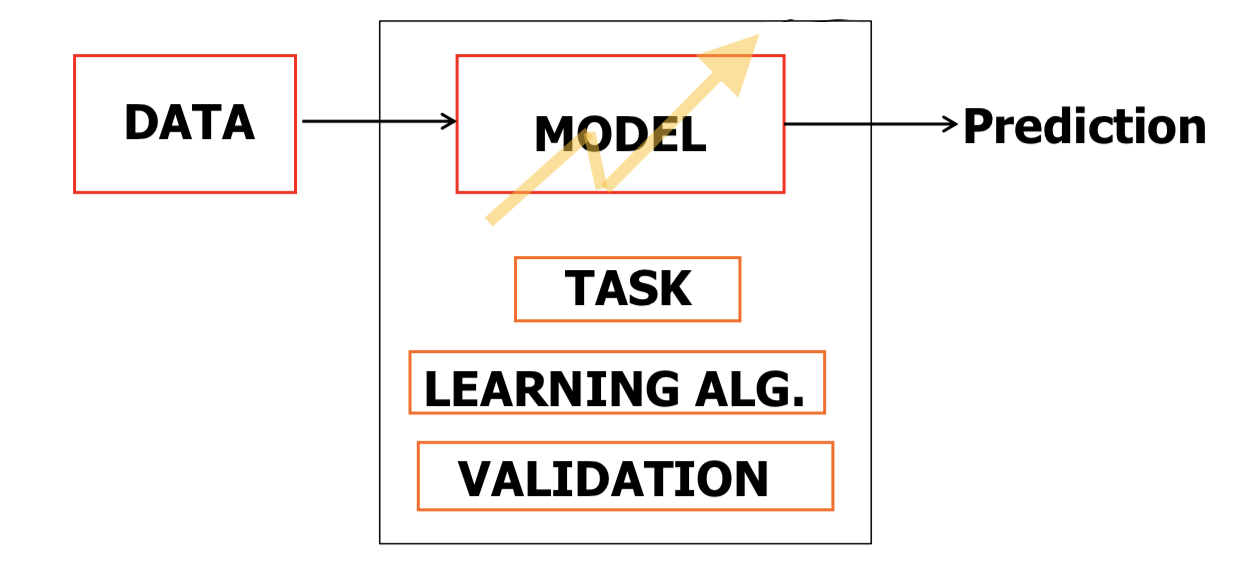
\includegraphics[scale=0.5]{Images/modelloML.png}
\end{figure}

\begin{itemize}
    \item DATA: i dati li ricaviamo dalle osservazioni del mondo
    \item MODEL: i dati passano attraverso un modello. Il modello non è fissato: ha dei parametri liberi, modificabili per fornire le predizioni in modo che siano quelle che vorremmo che fossero fornite.
    \begin{itemize}
        \item TASK: Supervised o Unsupervised Learning
        \item LEARNING ALGORITHM: algoritmo che cerca la soluzione in uno spazio di stati
        \item VALIDATION: valutazione statistica del modello (quanto riesce ad essere accurato sui dati futuri). 
    \end{itemize}
    \item PREDICTION: è l'output restituito dal modello
\end{itemize} 
"Apprendere" viene visto come una approssimazione di una funzione sconosciuta ricavata dagli esempi. 

\subsubsection{Riconoscimento caratteri}
Un esempio "pilota" che possiamo fare è il riconoscimento di caratteri scritti a mano. Il problema è racchiuso nel riconoscere una funzione che passa per un insieme di punti. Come input abbiamo una collezione di immagini di caratteri scritti a mano. Il problema è costruire un modello che riceve in input queste matrici di 8x8 pixel e come output restituire la cifra riconosciuta.
\begin{figure}[H]
    \centering
    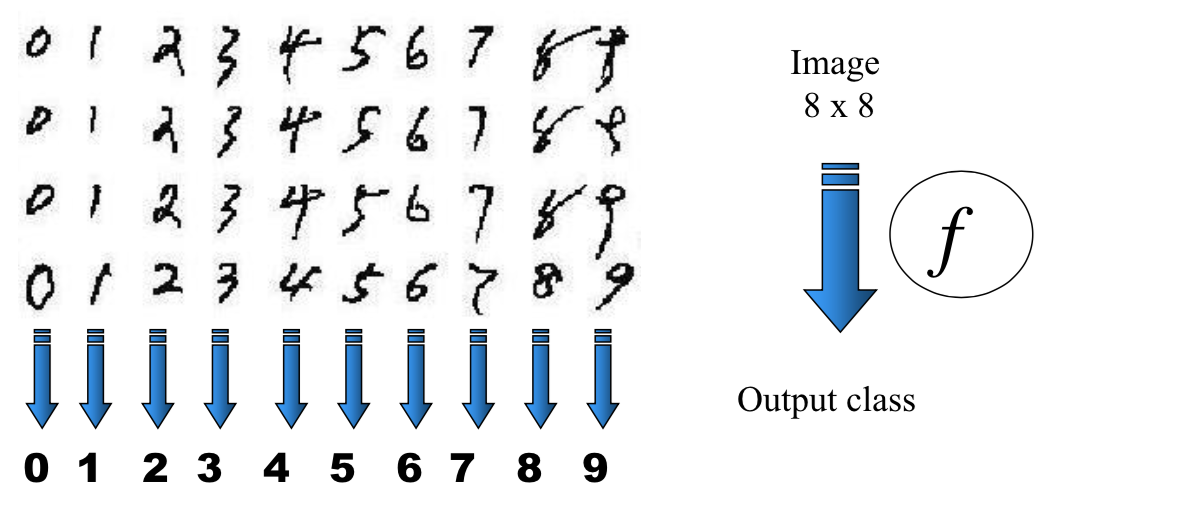
\includegraphics[scale=0.5]{Images/caratteririconoscimento.png}
\end{figure}
Non sappiamo quale sia la funzione, perché in quel caso la scriveremmo direttamente in un algoritmo. Cerchiamo quindi di approssimare una funzione facendo restituire come output una classificazione della matrice di pixel. Il problema di classificazione è dato dalla formalizzazione della soluzione esatta, poiché ci possiamo trovare con dati rumorosi o ambigui. Risulta però facile raccogliere collezioni di esempi etichettati, cioè esempi con soluzioni associate. \newline
Generalizzando il problema possiamo usare la tecnica del Supervised Learning. In particolare abbiamo in input uno spazio contentente "x" dati etichettati, dobbiamo costruire una funzione generale a partire dagli esempi e come output dare una categoria o valori reali. 

\subsection{TASK: Supervised Learning}
Il Supervised Learning è una tecnica di apprendimento automatico che mira a istruire un sistema informatico, in modo da consentirgli di elaborare automaticamente previsioni sui valori di uscita di un sistema rispetto ad un input sulla base di una serie di esempi ideali, costituiti da coppie di input e di output, che gli vengono inizialmente forniti. \newline
Quindi vengono dati esempi di training nella forma di coppie $<input,output>$ = $<x,d>$ (esempi etichettati) per la creazione di una funzione sconosciuta f. Definiamo il valore target come il valore "d" che vogliamo ottenere come output (e che ci viene dato tramite gli esempi). \newline
Bisogna trovare una buona approssimazione di f, cioè una ipotesi h che può essere usata per predire l'output sui dati sconosciuti $x'$. \newline
L'obiettivo è dare in output una etichetta numerica o la classificazione del dato. 
\begin{itemize}
    \item Classificazione: la funzione a valori discreti f(x) restituisce la presunta classe corretta per x.
    \item Regressione: consiste nell'approssimare a valori reali la funzione target.
\end{itemize}
Entrambi sono compiti di approssimazione di funzione.

\subsection{TASK: UNsupervised Learning}
L'apprendimento non supervisionato è una tecnica di apprendimento automatico che consiste nel fornire al sistema informatico una serie di input (esperienza del sistema) che egli riclassificherà ed organizzerà sulla base di caratteristiche comuni per cercare di effettuare ragionamenti e previsioni sugli input successivi. Abbiamo quindi un TR set che è un insieme di dati non etichettati, il compito è quello di raggruppare i dati in insiemi consistenti. I principali algoritmi sono:
\begin{itemize}
    \item Clustering: raggruppamento di elementi omogenei in un insieme di dati (cluster) identificando un centroide.
    \item Dimensionality reduction / Visualization / Preprocessing
    \item Modeling the data density
\end{itemize}
\begin{figure}[H]
    \centering
    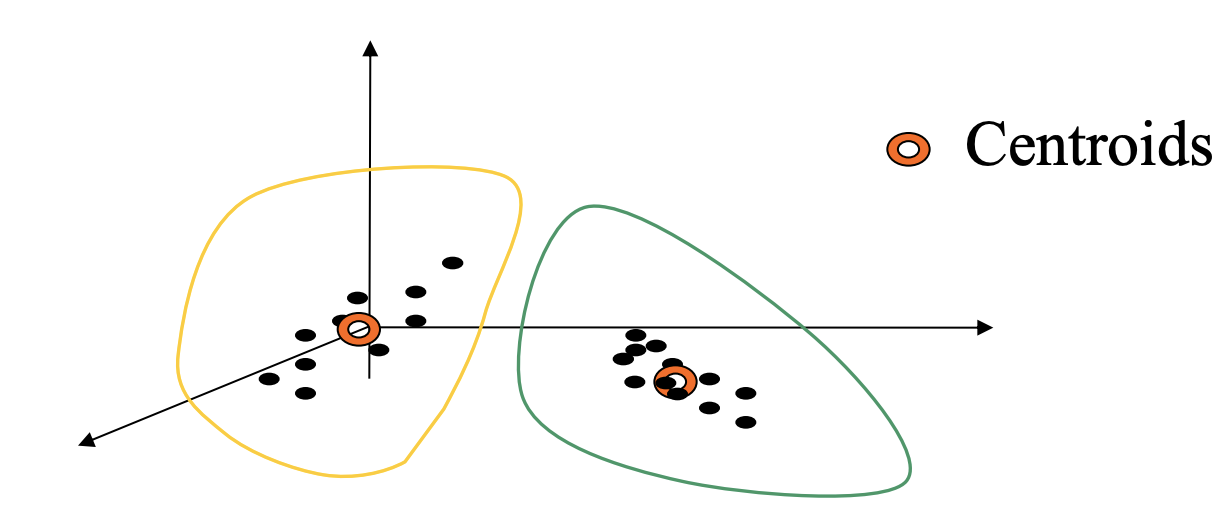
\includegraphics[scale=0.4]{Images/clustering.png}
    \caption{Esempio di clustering}
\end{figure}

\subsection{MODEL}
Il compito è quello di catturare e descrivere le relazioni tra i dati sulla base del TASK. Il modello definisce la classe delle funzioni che la macchina può implementare (cioè definisce lo spazio delle ipotesi H). \newline
Concetti utili: 
\begin{itemize}
    \item Training examples: fanno parte del Supervised Learning ed é un insieme di esempi nella forma (x,f(x)) dove x è un vettore di caratteristiche e f(x) è il valore obiettivo.
    \item Target function: la funzione obiettivo f il piú possibile corretta
    \item Hypotesis: è una funzione h che è ritenuta di essere simile a f. La funzione h è data in un linguaggio capace di esprimere le relazioni tra i dati.
    \item Hypoteses space: è lo spazio di tutte le ipotesi che possono essere output dell'algoritmo. É dove cerchiamo la funzione h. 
\end{itemize}
I linguaggi per le ipotesi h devono saper esprimere modelli di ML: ad esempio la logica del primo ordine, equazioni numeriche oppure calcolo delle probabilità.

\subsubsection{Esempi di Modelli}
\begin{itemize}
    \item Modelli Lineari: la rappresentazione dello spazio delle ipotesi H definisce uno spazio continuo parametrizzato di potenziali ipotesi. Come parametro abbiamo w, ed ogni assegnamento di w è una ipotesi differente. (es: $h_w(x)=w_1x+w_0$)
    \item Regole simboliche: lo spazio delle ipotesi è basato su rappresentazioni discrete, sono possibili differenti regole come ad esempio: if ($x_1$=0 and $x_2$=1) then h(x)=1 else h(x)=0
    \item Modelli probabilistici: stimare p(x,y)
    \item Approcci basati sull'istanza: confronta le nuove istanze del problema con le istanze osservate durante l'addestramento, che sono state memorizzate. Si chiama basato sull'istanza perché costruisce ipotesi direttamente dalle istanze di addestramento stesse.
\end{itemize}

\subsection{LEARNING ALGORITHM}
Gli algoritmi di apprendimento si basano su DATA, TASK e MODEL. L'euristica consiste nella ricerca delle migliori ipotesi nello spazio delle ipotesi H, cioè la miglior approssimazione della funzione obiettivo f sconosciuta (ad esempio i parametri liberi del modello vengono adattati al compito da svolgere: il miglior w nel modello lineare, la miglior regola per regole simboliche, ecc...). H potrebbe non coincidere con l'insieme di tutte le possibili funzioni e la ricerca può non risultare esaustiva, per questo bisogna fare assunzioni (vedremo in seguito il ruolo dell'Inductive Bias).
\begin{figure}[H]
    \centering
    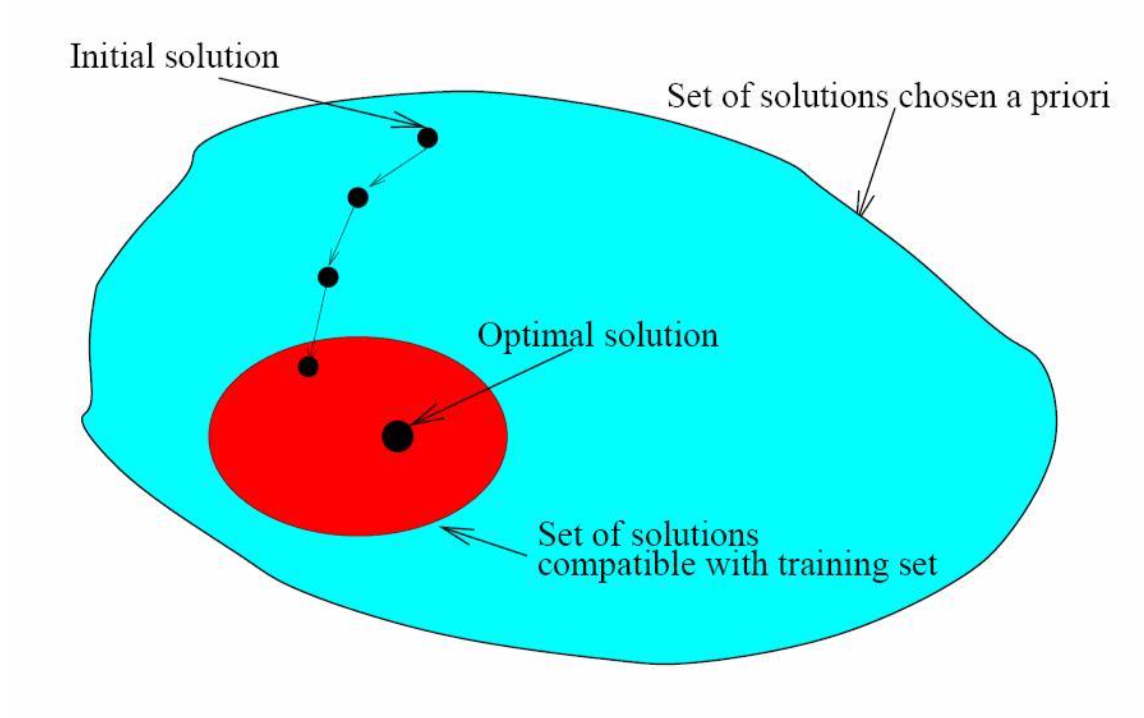
\includegraphics[scale=0.4]{Images/learningalgo.png}
\end{figure}

\subsection{VALIDATION - Generalizzazione}
L'apprendimento può essere quindi definito come la ricerca una buona funzione, in uno spazio di funzioni restituito da dati conosciuti. "Buona funzione" considerando l'errore di generalizzazione (o capacità di generalizzazione) cioè quanto accuratamente il modello prevede nuovi campioni di dati. La generalizzazione è cruciale in ML $\rightarrow$ strumenti corretti di ML.
\begin{itemize}
    \item Fase di apprendimento (training, fitting): costruire il modello dai dati di training conosciuti (Training Set).
    \item Fase predittiva (test): si applica la funzione costruita a un nuovo esempio. Si prende in input x, si computa la risposta dal modello e confrontiamo l'output con il nostro target (che il modello non ha mai visto). Si esegue una valutazione dell'ipotesi predittiva, ad esempio la valutazione della capacità di generalizzazione (valutazione statistica del modello, quanto riesce ad essere accurato sui dati futuri). É bene notare che essere performanti in ML significa predire accuratamente, cioè la performance é stimata dagli errori effettuati calcolando la funzione sul Test Set (che é diverso dal Training set!).
\end{itemize}

\section{Concept Learning}
Il Concept Learning anche noto come apprendimento di categoria é definito come "la ricerca di attributi che possono essere utilizzati per distinguere i modelli dai non modelli di varie categorie". Più semplicemente, i concetti sono le categorie che ci aiutano a classificare oggetti, eventi o idee, basandoci sul fatto che ogni oggetto, evento o idea ha un insieme di caratteristiche rilevanti comuni. In un compito di Concept Learning, una macchina apprende come classificare degli oggetti mostrandole prima una serie di esempi associati alle loro etichette di classe. La macchina semplifica quello che ha osservato "condensandolo" sotto forma di un esempio. Questa versione semplificata di ciò che è stato appreso viene quindi applicata a esempi futuri. \newline
Lavoriamo in uno spazio discreto strutturato come lo spazio delle ipotesi, useremo come rappresentazione la congiunzione di letterali e vedremo algoritmi come Find-S ed Candidate Elimination. Praticamente in questa sezione andremo ad vedere in cosa consiste la classificazione del Supervised Learning, cioè come la funzione f(x) restituisce la presunta classe corretta per x.

\begin{quote}
    Concept Learning: dedurre una funzione booleana (con dominio X e codominio \{t,f\}) da esempi di allenamento positivi e negativi (dove X é lo spazio che contiene le istanze)
\end{quote}
Un Training Example é definito come coppia <x,c(x)> (le coppie sono contenute nel Training Set). \newline
L'ipotesi h: $X \rightarrow \{0,1\}$ soddisfa x se h(x)=1. \newline
Una ipotesi h é consistente con un esempio di allenamento <x,c(x)> se h(x)=c(x) con x appartenente a X. É consistente anche con D\footnote{é sempre il Training Set insieme degli esempi} se h(x)=c(x) per ogni esempio di allenamento <x,c(x)> in D.
\clearpage

\subsubsection{Esempio: Apprendimento Funzione Booleana}
\begin{figure}[H]
    \centering
    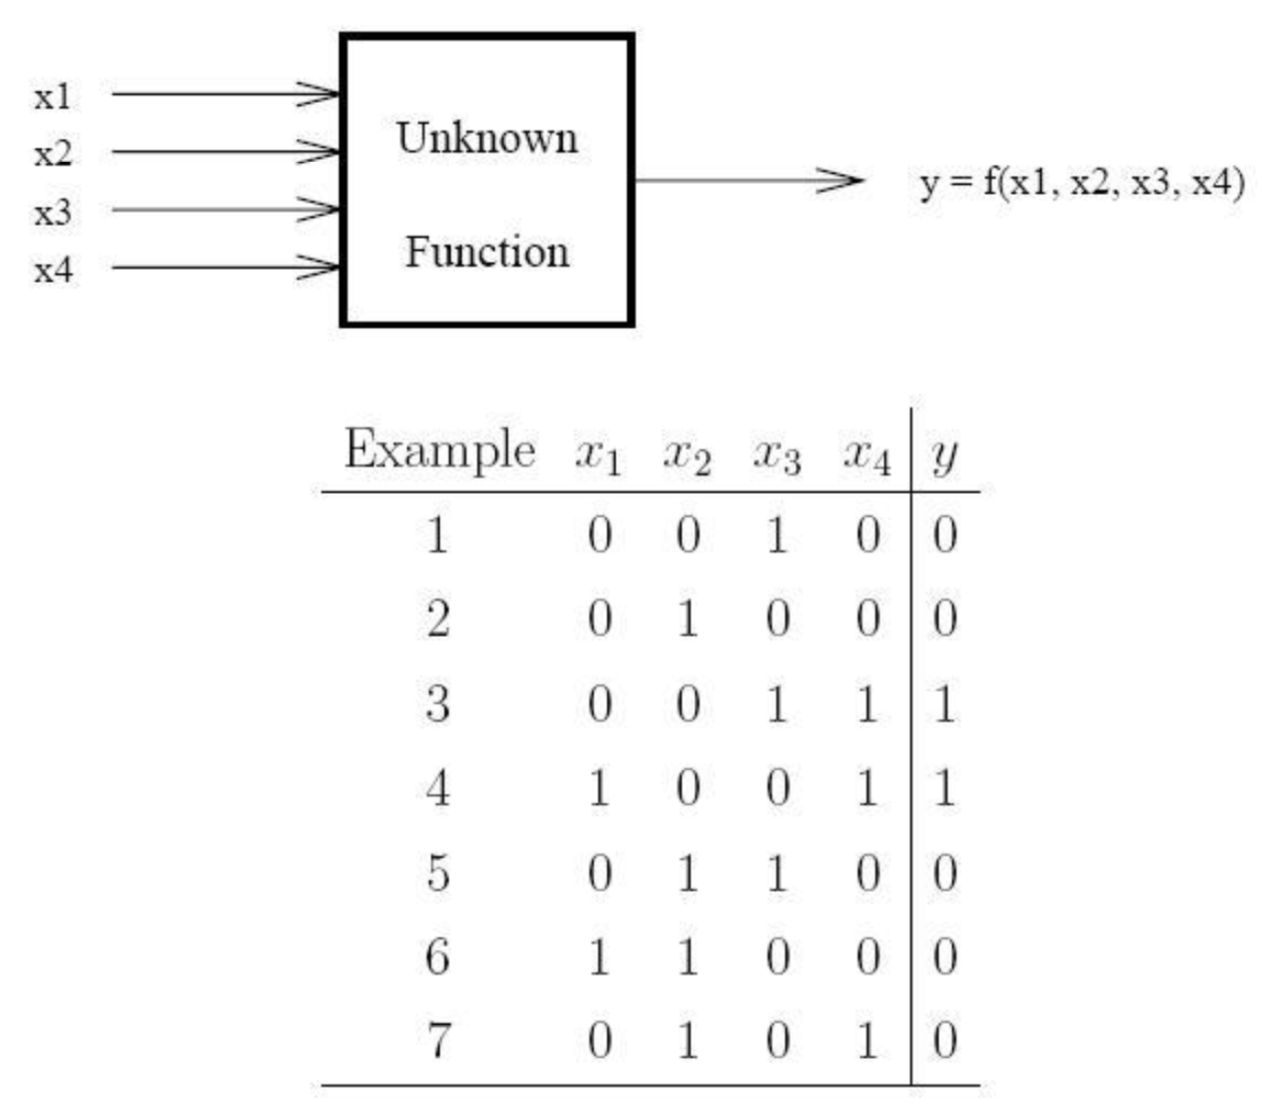
\includegraphics[scale=0.4]{Images/esempiofunzionebooleana.png}
\end{figure}
Questo é un problema mal posto poiché potremmo violare l'esistenza, unicità o stabilità della soluzione. Come possiamo vedere dall'immagine abbiamo in input 4 variabili e in output un singolo valore. Nella tabella troviamo il nostro training set (D) e il nostro compito é quello di trovare la funzione che dati in input quei valori restituisce l'output definito dalla tabella. Ci sono $2^{2^4}$ possibili funzioni booleane per 4 ingressi, questo perché abbiamo $2^4$ possibili ingressi e per ognuno possiamo rispondere 0 o 1. Non possiamo sapere quale sia la funzione corretta fino a che non abbiamo visto tutte le possibili coppie di input/output. Dopo aver analizzato i nostri 7 esempi ci rimangono ancora $2^9$ possibilità. Nel caso generale per input/output binari la formula é $|H| = 2^{numeroistanze} = 2^{2^n}$ dove $|H|$ é la dimensione dello spazio delle ipotesi ed n é la dimensione dell'input. \newline
Lavoreremo con uno spazio delle ipotesi ristretto: partiamo scegliendo uno spazio delle ipotesi H che é considerevolmente più piccolo dello spazio di tutte le possibili funzioni. \newline Vedremo: 
\begin{itemize}
    \item proposizioni formate da solo "and" (regole congiuntive) in uno spazio di ipotesi H finito e discreto
    \item funzioni lineari, in uno spazio di ipotesi H continuo e infinito
\end{itemize}

\subsection{Regole Congiuntive}
Quante h diverse possiamo avere? Cioè quante semplici regole congiuntive? \newline
Nel caso generale:
\begin{itemize}
    \item Letterali positivi: ad esempio $h_1 = l_2$, $h_2=(l_1 \land l_2)$, $h_3 = true$ ecc... sono semplici regole congiuntive. Abbiamo ridotto lo spazio delle ipotesi così da ottenere $|H| = 2^n$ basti immaginare $l_i$ come una stringa di bit di lunghezza n.
    \item Letterali: (di cui fa parte anche il not($l_i$)) ottenendo uno spazio delle ipotesi di dimensione $3^n+1$
\end{itemize}
Vedremo come organizzare e cercare in modo efficiente attraverso uno spazio di ipotesi, sfruttando algoritmi per un insieme di ipotesi molto limitato semplificandoci il lavoro usando dati non rumorosi.

\subsection{Problema: Enjoy Sport}
Concept: "giorni in cui piace fare sport acquatici" \newline
Task: predire il valore di "Enjoy Sport" per un giorno arbitrario in base ai valori degli attributi.
\begin{table}[H]
\centering
\begin{tabular}{l|l|l|l|l|l|l}
Sky & Temp & Humid & Wind & Water & Forecast & Enjoy Sport? \\ \hline
Sunny & Warm & Normal & Strong & Warm & Same & Yes \\
Sunny & Warm & High & Strong & Warm & Same & Yes \\
Rainy & Cold & High & Strong & Warm & Change & No \\
Sunny & Warm & High & Strong & Cool & Change & Yes
\end{tabular}
\end{table}
Una riga della tabella é una istanza.

\subsection{Rappresentare le Ipotesi}
L'ipotesi h é una congiunzione di vincoli sugli attributi. Ogni vincolo può essere:
\begin{itemize}
    \item Uno specifico valore: ad esempio Water = Warm
    \item Un valore irrilevante: ad esempio Water = ?
    \item Nessun valore consentito (ipotesi nulla): ad esempio Water = 0
\end{itemize}
Esempio di ipotesi h:
\begin{table}[H]
\centering
\begin{tabular}{l|l|l|l|l|l}
Sky & Temp & Humid & Wind & Water & Forecast \\ \hline
Sunny & ? & ? & Strong & ? & Same
\end{tabular}
\end{table}
corrispondente alla funzione booleana
\begin{quote}
    $Sky=Sunny \land Wind=Strong \land Forecast=Same$
\end{quote}
L'ipotesi più specifica (risponde sempre false) e più generale (risponde sempre true) sono rispettivamente
\begin{table}[H]
\centering
\begin{tabular}{l|l|l|l|l|l}
Sky & Temp & Humid & Wind & Water & Forecast \\ \hline
0 & 0 & 0 & 0 & 0 & 0 \quad //specifica \\
? & ? & ? & ? & ? & ? \quad //generale
\end{tabular}
\end{table}

\subsection{TASK del Concept Learning}
Vengono dati:
\begin{itemize}
    \item Le istanze X: i possibili giorni vengono descritti da attributi Sky, Temp, Humid, Wind, Water e Forecast.
    \item Funzione Target: c: EnjoySport $X \rightarrow \{0,1\}$.
    \item Spazio delle ipotesi (H): insieme finito di coniunzioni di letterali
    \item Esempi di allenamento (D): esempi positivi e negativi: $<x_1, c(x_1)>, ..., <x_n, c(x_n)>$
\end{itemize}
Bisogna trovare:
\begin{itemize}
    \item Una ipotesi h in H tale che h(x)=c(x) per tutti gli x in X
\end{itemize}
L'apprendimento sta nella ricerca nello spazio delle ipotesi H.

\subsection{Apprendimento Induttivo}
\begin{quote}
    Ipotesi Apprendimento Induttivo: "Qualsiasi ipotesi trovata per approssimare la funzione target sugli esempi di allenamento, approssimerà anche la funzione target sugli esempi non osservati". Ma purtroppo non è detto che il Training Set sia corretto (dati rumorosi, ...)
\end{quote}
Quindi h(x)=c(x) per ogni x in D (funzione consistente con il training set) ma h(x)=c(x) per ogni x in X? Problema fondamentale del ML.

\subsection{Qual é il numero di istanze, concetti e ipotesi di un problema?}
\begin{itemize}
    \item Sky: Sunny, Cloudy, Rainy
    \item Temp: Warm, Cold
    \item Humid: Normal, High
    \item Wind: Strong, Weak
    \item Water: Warm, Cold
    \item Forecast: Same, Change
\end{itemize}
La scelta della rappresentazione di H determina lo spazio di ricerca! \newline
Numero di possibili istanze: 3*2*2*2*2*2 = 96 \newline
Numero di concetti distinti: $2^{96} = 2^{numeroistanze}$ \newline
Numero di ipotesi sintatticamente distinte: 5*4*4*4*4*4 (poiché per ogni attributo devo aggiungere 0 o ?) \newline
Numero di ipotesi semanticamente distinte: 1+4*3*3*3*3*3 (poiché le ipotesi con almeno uno 0 sono equivalenti a false, i valori sono in and!) \newline
Strutturare uno spazio di ricerca può aiutare a cercare in modo piú efficiente.

\subsection{Da ordine generale a ordine specifico}
Consideriamo due ipotesi
\begin{enumerate}
    \item $h_1$ = $<Sunny,?,?,Strong,?,?>$
    \item $h_2$ = $<Sunny,?,?,?,?,?>$
\end{enumerate}
L'insieme di istanze coperte da $h_1$ e da $h_2$ sono differenti, infatti $h_2$ impone meno vincoli rispetto a $h_1$ e quindi classifica più istanze x positive ($h_2(x)$=1).
\begin{quote}
    Siano $h_j$ e $h_k$ funzioni booleane definite su X. $h_j$ é più generale o equivalente a $h_k$ ($h_j \geq h_k$) se solo se $\forall x \in X : [(h_k(x)=1) \rightarrow (h_j(x)=1)]$
\end{quote}
Possiamo sfruttare questo ordine parziale per organizzare più efficientemente la nostra ricerca in H.
\begin{figure}[H]
    \centering
    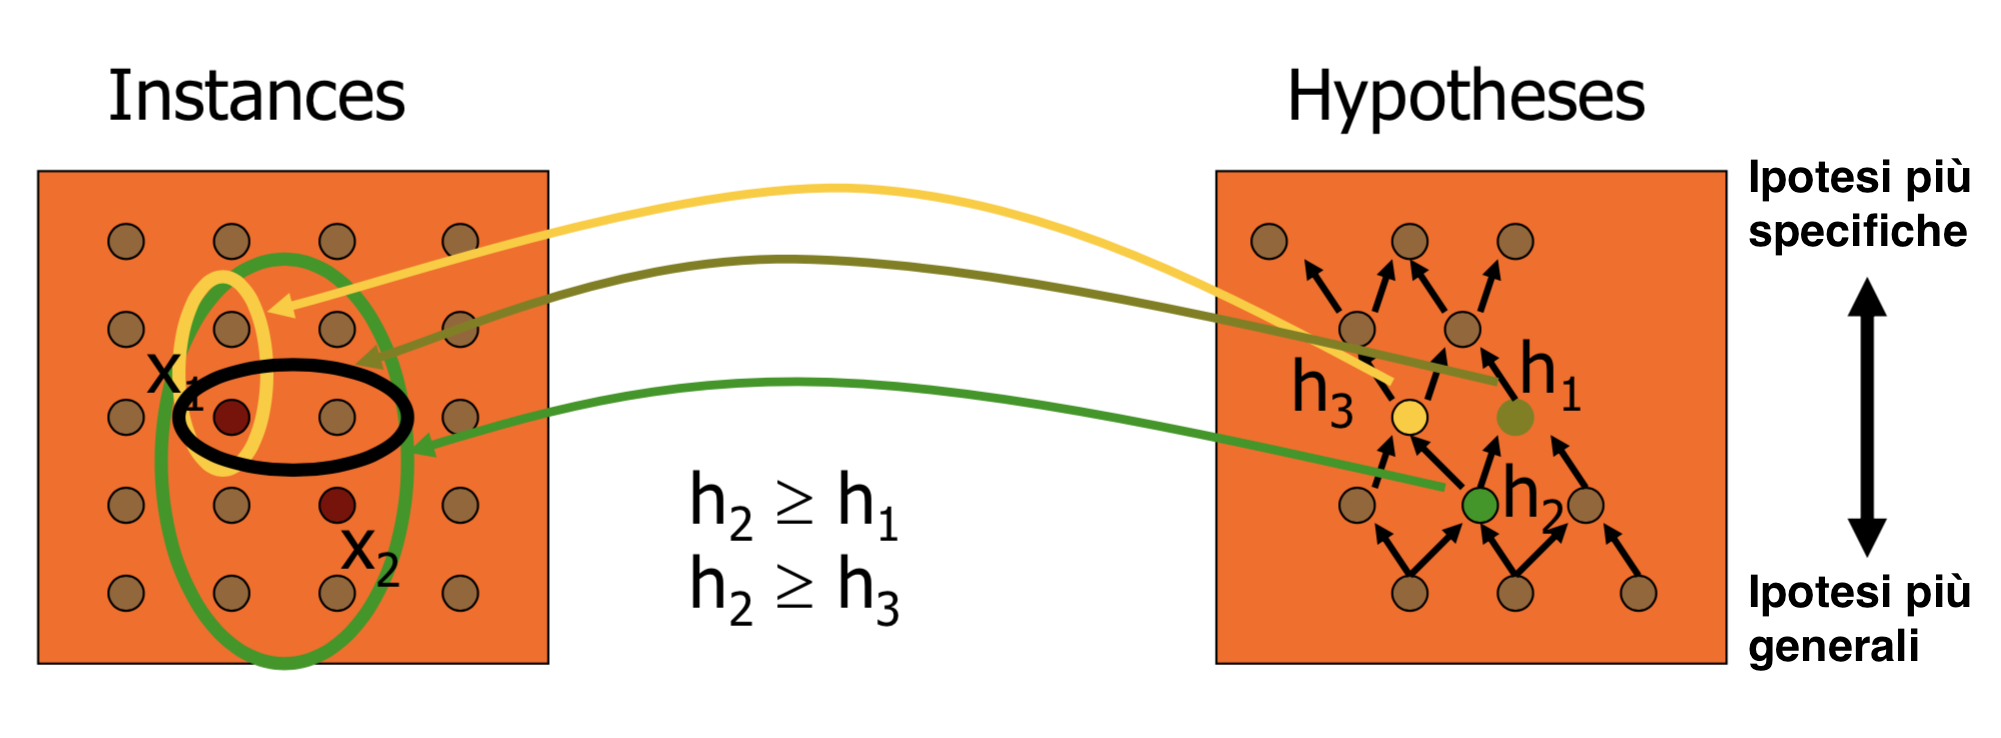
\includegraphics[scale=0.4]{Images/partialorder.png}
    \caption{Partial Order}
\end{figure}
Istanze:
\begin{itemize}
    \item $x_1$ = $<Sunny,Warm,High,Strong,Cool,Same>$
    \item $x_2$ = $<Sunny,Warm,High,Light,Warm,Same>$
\end{itemize}
Ipotesi:
\begin{itemize}
    \item $h_1$ = $<Sunny,?,?,Strong,?,?>$
    \item $h_2$ = $<Sunny,?,?,?,?,?>$
    \item $h_3$ = $<Sunny,?,?,?,Cool,?>$
\end{itemize}

\subsection{Algoritmo Find-S (Specific)}
L'algoritmo Find-S sfrutta l'ordine parziale di gestione per cercare in modo efficiente una h consistente (senza elencare esplicitamente ogni h in H).
\begin{enumerate}
    \item Inizializza h con l'ipotesi più specifica nello spazio delle ipotesi H ($h_0 = <0, 0, 0, 0, 0, 0>$)
    \item Prendo il prossimo esempio di training:
        \begin{itemize}
            \item Per ogni attributo $a_i$ dell'ipotesi h, se $a_i$ é soddisfatto in h da x allora non fare nulla (quindi se l'esempio é negativo non ci sono cambiamenti sull'ipotesi), altrimenti se $a_i$ NON é soddisfatto e l'esempio é positivo, sostituisci $a_i$ con il prossimo vincolo più generale soddisfatto da x. \newline 
            Ripeto il passaggio per ogni esempio positivo.
        \end{itemize}
    \item Viene dato in output l'ipotesi h
\end{enumerate}
L'algoritmo parte dall'ipotesi più specifica, poi scende in maniera conservativa (generalizza il minimo possibile) in modo da rimanere consistente sui positivi, e di conseguenza contemporaneamente sui negativi. Trovo un'ipotesi che copre tutti i positivi e tutti i negativi. In questo modo evito di esplorare tutto H, scorrendo solo una volta il training set, perché si segue il Partial Order.
\subsubsection{Esempio su Enjoy Sport}
\begin{enumerate}
    \item $h_0 = <0, 0, 0, 0, 0, 0>$
    \item $x_1 = <Sunny, Warm, Normal, Strong, Warm, Same>$ \quad questo esempio é positivo\footnote{l'esempio é preso dalla tabella a pagina 10} e $h_0$ non é soddisfatta perché False. Quindi devo prendere i vincoli più generali da $x_1$ e metterli in h, in questo caso sono le singole istanze poiché tutte piú generali di 0.
    \item $h_1 = <Sunny, Warm, Normal, Strong, Warm, Same>$
    \item $x_2 = <Sunny, Warm, \textcolor{red}{High}, Strong, Warm, Same>$ \quad esempio positivo, notiamo che High é in constrasto con Normal. Quindi cambio quell'attributo con uno piú generale, in questo caso é "?".
    \item $h_2 = <Sunny, Warm, ?, Strong, Warm, Same>$
    \item $x_3 = <Rainy, Cold, High, Strong, Warm, Change>$ \quad esempio é negativo quindi non faccio nulla
    \item $h_3 = <Sunny, Warm, ?, Strong, Warm, Same>$
    \item $x_4 = <Sunny, Warm, High, Strong, \textcolor{red}{Cool}, \textcolor{red}{Change}>$ \quad esempio positivo
    \item $h_3 = <Sunny, Warm, ?, Strong, ?, ?>$
\end{enumerate}

\subsubsection{Proprietà di Find-S}
Lo spazio delle ipotesi é rappresentato come congiunzione di attributi (molto limitativo), l'algoritmo darà in output l'ipotesi più specifica, nello spazio H, che é consistente con gli esempi positivi del training set. L'ipotesi di output h sarà anche consistente con gli esempi negativi, a condizione che il concetto target sia contenuto in H. Scegliamo l'ipotesi più specifica poichè nel caso in cui ci fossero diverse ipotesi consistenti con gli esempi di training, Find-S trova la più specifica.

\subsubsection{Aspetti negativi di Find-S}
Non so se il sistema di apprendimento converga con il concetto target, nel senso che non è in grado di determinare se ha trovato l'unica ipotesi coerente con gli esempi di allenamento. Inoltre non so quando i dati di allenamento sono incoerenti, in quanto ignora gli esempi di allenamento negativi $\rightarrow$ nessuna tolleranza al rumore sui dati!

\subsection{Version Spaces}
Find-S fornisce una singola ipotesi da H che è coerente con gli esempi di allenamento, questa è solo una delle tante ipotesi da H che potrebbero adattarsi ugualmente bene ai dati di allenamento. L'idea é quindi quella di dare in output l'insieme di tutte le possibili h consistenti con D.
\begin{quote}
    Il Version Space $VS_{H,D}$ rispetto allo spazio delle ipotesi H e il training set D, é il sottoinsieme delle ipotesi prese da h coerenti con tutti gli esempi di training: \newline $VS_{H,D} = \{h \in H | Consistent(h,D)\}$ \newline 
    dove $Consistent(h,D) = \forall<x,c(x)> \in D | h(x)=c(x)$
\end{quote}
Si dice che un esempio x soddisfa l'ipotesi h quando h(x)=1, indipendentemente dal fatto che x sia un esempio positivo o negativo del concetto target. Tuttavia, se un tale esempio sia coerente con h dipende dal concetto target e, in particolare, se h(x)=c(x).
\clearpage

\subsection{Algoritmo List-Then-Eliminate}
L'algoritmo List-Then-Eliminate inizializza il Version Space con tutte le ipotesi contenute in H eliminando volta per volta tutte le ipotesi che non sono consistenti con gli esempi di training. Il Version Space si riduce quindi man mano che si osservano più esempi, fino a quando idealmente rimane solo un'ipotesi coerente con tutti gli esempi osservati, presumibilmente, questo è il concetto target desiderato. Se non sono disponibili dati sufficienti per restringere lo spazio l'algoritmo può generare l'intero insieme di ipotesi coerenti con i dati osservati. L'algoritmo List-Then-Eliminate può essere applicato ogni volta che lo spazio di ipotesi H è finito. Ha molti vantaggi, tra cui il fatto che è garantito il risultato di tutte le ipotesi coerenti con i dati di allenamento. Sfortunatamente, richiede un elenco esaustivo di tutte le ipotesi in H, un requisito non realistico per tutti gli spazi di ipotesi tranne quelli più banali.
\begin{enumerate}
    \item Iniziamo impostando il nostro Version Space con una lista contente ogni ipotesi in H
    \item Per ogni esempio di allenamento $<x,c(x)>$ rimuoviamo dal Version Space ogni ipotesi che é inconsistente con gli esempi di allenamento cioé $h(x)!\neq c(x)$
    \item Viene dato in output la lista delle ipotesi ora contenute nel Version Space
\end{enumerate}

\subsubsection{Esempio di Version Space}
\begin{figure}[H]
    \centering
    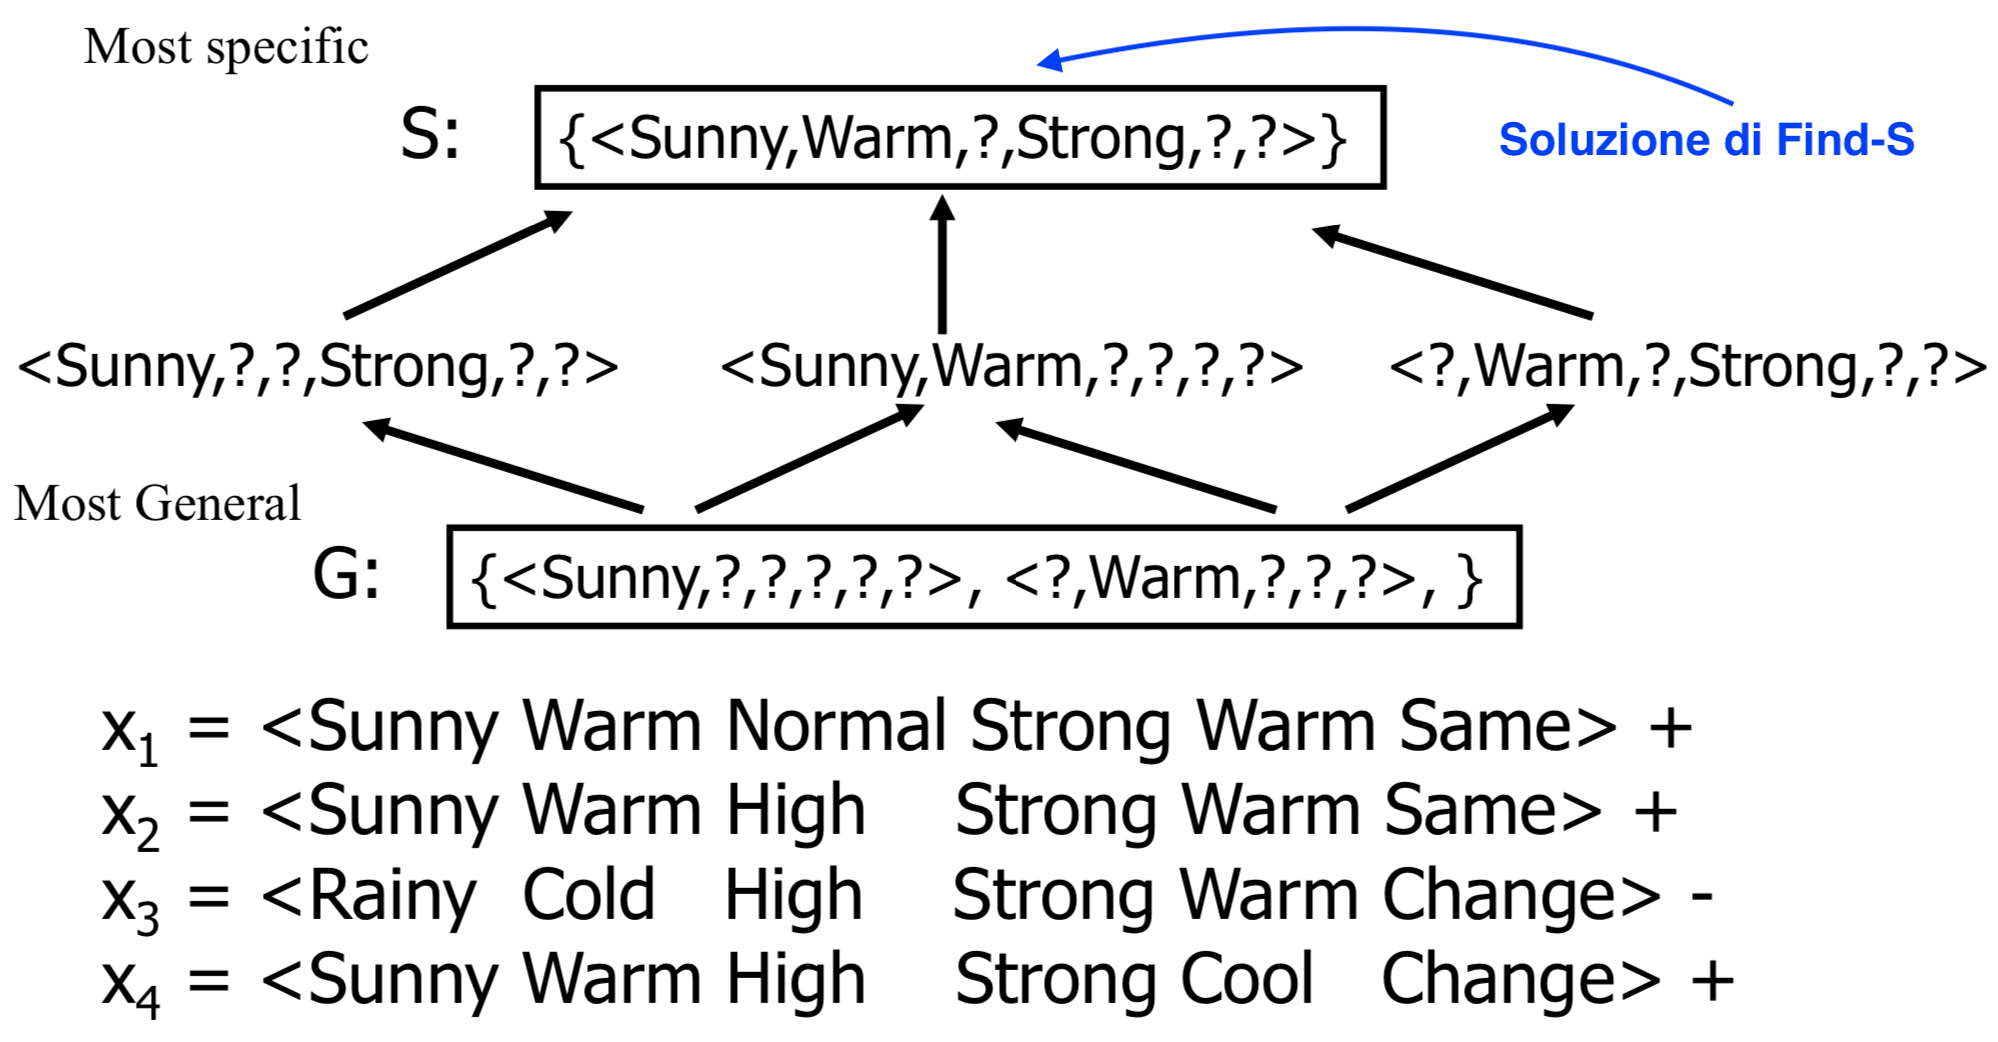
\includegraphics[scale=0.4]{Images/versionspacegs.png}
\end{figure}
Il Version Space dell'algoritmo viene rappresentato solo dal suo membro più generale G e dal più specifico S (che é la soluzione di Find-S!).
\begin{quote}
    Teorema: ogni membro del Version Space si trova tra: \newline 
    $VS_{H,D} = \{h \in H| (\exists s \in S) (\exists g \in G) (g \geq h \geq s)\}$
\end{quote}
dove $x \geq y$ significa x é piú generale o uguale a y.
\clearpage

\subsection{Algoritmo Candidate Elimination}
L'algoritmo di Candidate Elimination calcola il Version Space contenente tutte le ipotesi di H che sono coerenti con una sequenza osservata di esempi di addestramento. L'algoritmo calcola il Version Space senza elencarne esplicitamente tutti i suoi membri, ciò si ottiene utilizzando l'ordinamento più generale che parziale e mantenendo una rappresentazione compatta dell'insieme di ipotesi coerenti. \newline
Inizia inizializzando il Version Space sull'insieme di tutte le ipotesi in H, cioè inizializzando il set di limiti G per contenere l'ipotesi più generale in H $G_0 = <?, ?, ?, ?, ?, ?>$ e inizializzando il set di limiti S per contenere l'ipotesi più specifica $S_0 = <0, 0, 0, 0, 0, 0>$. Questi due insiemi di limiti delimitano l'intero spazio delle ipotesi, poiché ogni altra ipotesi in H è sia più generale di $S_0$ sia più specifica di $G_0$. Dopo che tutti gli esempi sono stati elaborati, lo spazio versione calcolato contiene tutte le ipotesi coerenti con questi esempi.
\begin{enumerate}
    \item Inizializza G con l'insieme di ipotesi massimamente generali in H $G_0 = <?, ?, ?, ?, ?, ?>$
    \item Inizializza S con l'insieme di ipotesi massimamente specifiche in H $S_0 = <0, 0, 0, 0, 0, 0>$
    \item Per ogni esempio di training $d=<x,c(x)>$:
        \begin{itemize}
            \item se d é positivo: 
                \begin{itemize}
                    \item Rimuovere da G ogni ipotesi incompatibile con d
                    \item per ogni ipotesi s in S che non è coerente con d: (Generalizziamo S)
                        \begin{itemize}
                        \item Rimuovere s da S
                        \item Aggiungi a S tutte le minime generalizzazioni h di s tali che h é consistente con d e alcuni membri di G sono più generali di h
                        \item Rimuovi da S ogni ipotesi più generale di un'altra ipotesi in S
                        \end{itemize}
                \end{itemize}
            \item se d é negativo: 
                \begin{itemize}
                    \item Rimuovere da S ogni ipotesi incompatibile con d
                    \item per ogni ipotesi g in G che non è coerente con d: (Specializziamo G)
                        \begin{itemize}
                        \item Rimuovere g da G
                        \item Aggiungi a G tutte le minime specializzazioni h di g tali che h é consistente con d e alcuni membri di S sono più specifici di h
                        \item Rimuovi da G ogni ipotesi meno generale di un'altra ipotesi in G
                        \end{itemize}
                \end{itemize}
        \end{itemize}
\end{enumerate}

\subsubsection{Esempio di Candidate Elimination}
\begin{figure}[H]
    \centering
    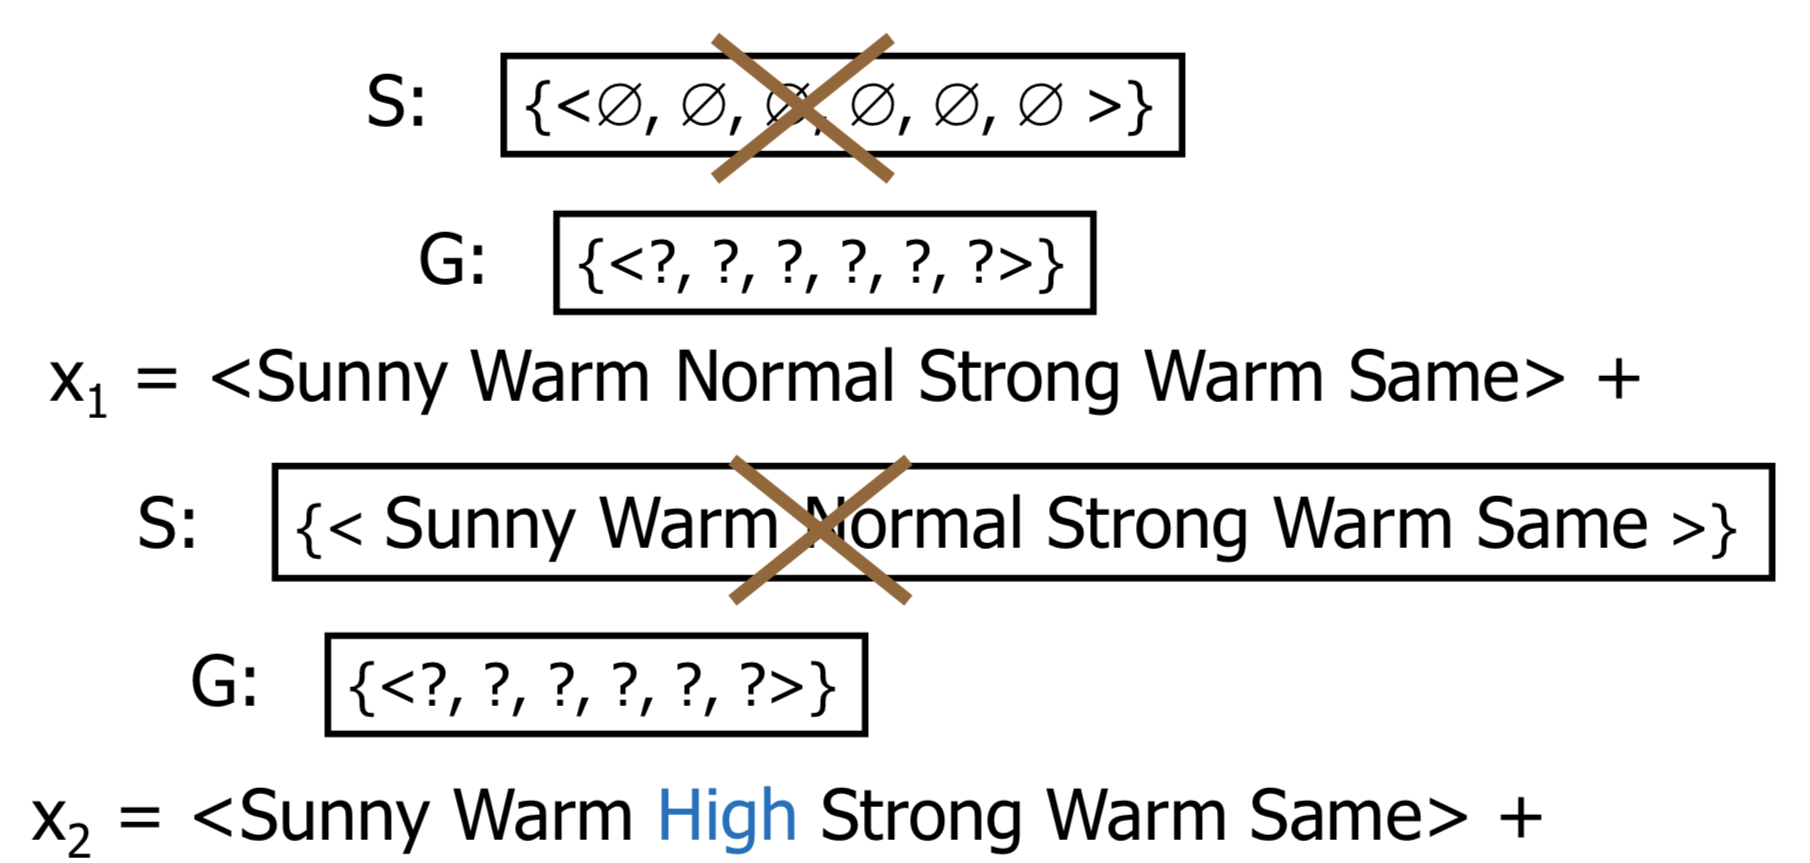
\includegraphics[scale=0.4]{Images/candidateelim1.png}
    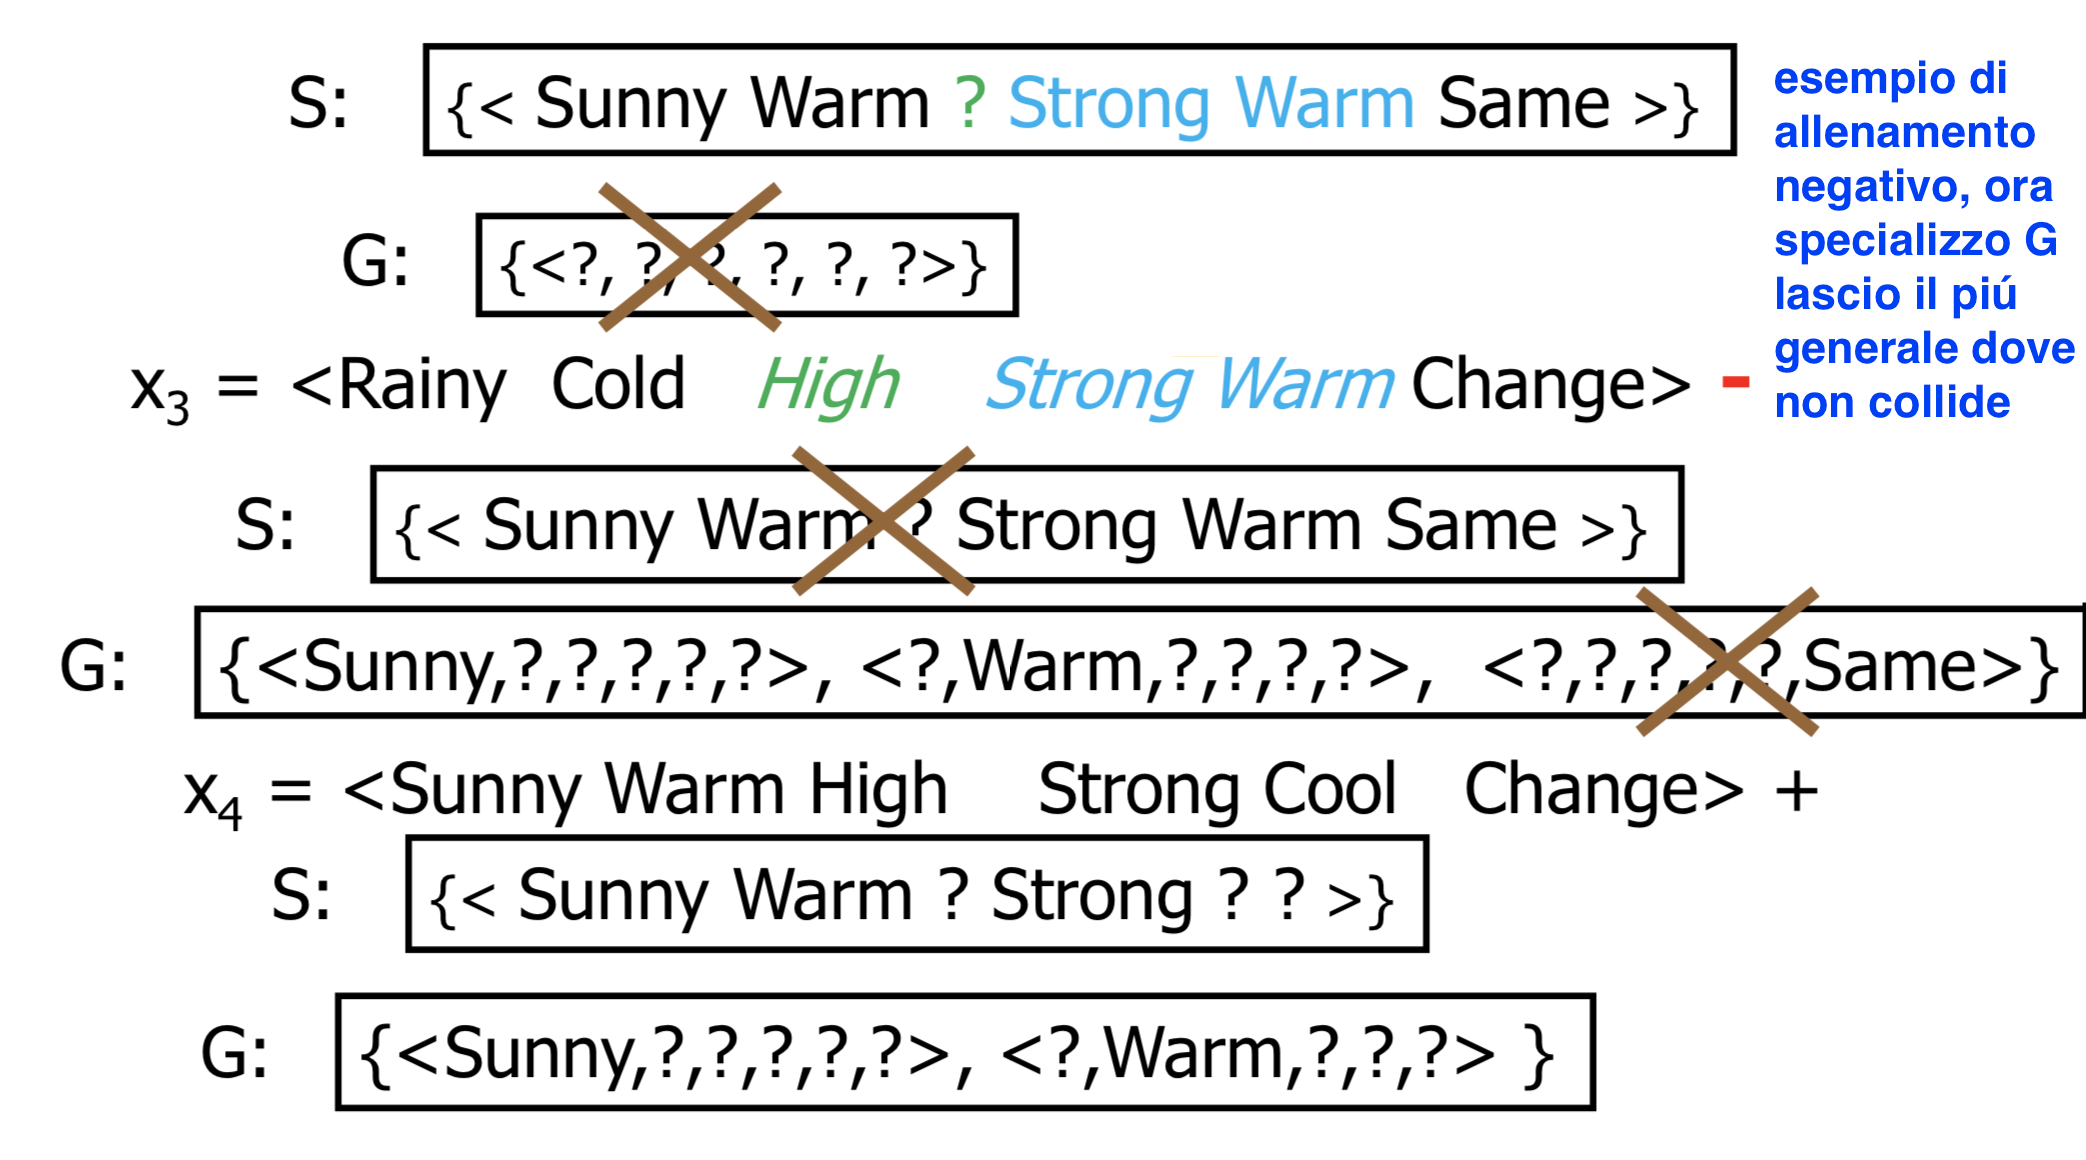
\includegraphics[scale=0.4]{Images/candidateelim2.png}
\end{figure}
G al passaggio 3 contiene le specializzazioni minime che mi permettono di coprire $x_3$ come negativa, senza rendere G più specializzato di S. S e G sono le "guardie" di tutti i positivi e di tutti i negativi trovati finora. Il fatto che se specializzo troppo G rendo false alcuni input già accettati, deriva dal partial order: intelligentemente il controllo di consistenza di tutti i vecchi input non è effettuato dall'algoritmo. Infatti, il limite S del Version Space costituisce un riepilogo degli esempi positivi riscontrati in precedenza che possono essere utilizzati per determinare se una ipotesi è coerente con questi esempi. Il limite G riassume le informazioni da esempi negativi riscontrati in precedenza. Ogni ipotesi più specifica di G è garantita per essere coerente con esempi negativi del passato.
\clearpage 

\section{Inductive Bias}
Il nostro spazio delle ipotesi non é in grado di rappresentare target disgiuntivi come ad esempio $(Sky=Sunny) \lor (Sky=Cloudy)$. \newline
Se avessimo due esempi del tipo: \newline
$x_1 = <Sunny, Warm, Normal, Strong, Cool, Change>$ (positivo) \newline
$x_2 = <Cloudy, Warm, Normal, Strong, Cool, Change>$ (positivo) \newline
troveremo che $S = \{ <?, Warm, Normal, Strong, Cool, Change> \}$ \newline
che é inconsistente con l'esempio $x_3 = <Rainy, Warm, Normal, Strong, Cool, Change >$ (negativo) \newline
trovando $S = \{\}$, cioé S collassa, perché la funzione target è fatta solo di and. \newline
PROBLEMA: abbiamo vincolato il sistema di apprendimento considerando solo ipotesi congiuntive. Abbiamo bisogno di uno spazio di ipotesi più espressivo.

\subsection{Sistema di apprendimento Unbiased}
La soluzione ovvia al problema di assicurare che il concetto target sia nello spazio di ipotesi H è di fornire uno spazio di ipotesi in grado di rappresentare ogni concetto insegnabile. \newline
Significa che H è l'insieme di tutti i possibili sottoinsiemi di X (questo insieme viene chiamato anche l'insieme di potenza P(X)). In EnjoySport $|H|=96$, $|P(X)|=2^{96}$ concetti distinti. Un'ipotesi può essere rappresentata con disgiunzioni, congiunzioni e negazioni delle nostre precedenti ipotesi. H sicuramente contiene il concetto target. Con questa modifica quali sono i nostri G e S? \newline
NUOVO PROBLEMA: il nostro algoritmo di apprendimento dei concetti non è ora in grado di generalizzare oltre gli esempi osservati. Assumiamo tre esempi positivi $(x_l, x_2, x_3)$ e due esempi negativi $(x_4, x_5)$. $S = \{(x_1 \lor x_2 \lor x_3) \}$ e $G = \{\neg (x_4 \lor x_5)\}$ $\rightarrow$ Non abbiamo generalizzazione, S sarà sempre la disgiunzione degli esempi positivi e G la disgiunzione di quelli negativi!
\begin{quote}
    Proprietà: un sistema di apprendimento non vincolato non è in grado di generalizzare \newline
    Prova: ogni nuova istanza verrà classificata positivamente precisamente da metà delle ipotesi nel Version Space e negativa dell'altra metà. Poiché H è l'insieme di potenza di X e sia $x_i$ una istanza non vista precedentemente, $\forall h$ consistente con $x_i(test)$, $\exists h'$ identico ad h con eccezione che $h'(x_i) \neq h(x_i)$ cioè $h \in VS \rightarrow h' \in VS$ (sono identici in D)
\end{quote}

\subsubsection{Il learning Unbiased é utile?}
Un sistema di apprendimento che non fa assunzioni preliminari riguardo all'identità del concetto target non ha basi razionali per classificare eventuali istanze non conosciute. Un sistema di apprendimento dovrebbe essere in grado di generalizzare a partire dai dati di allenamento al fine di classificare istanze mai viste precedentemente. Il "bias" non è solo assunto per efficienza, ma è necessario per la generalizzazione, tuttavia non ci dice quale sia la migliore soluzione per la generalizzazione.

\subsection{Definizione Formale di Inductive Bias}
Consideriamo:
\begin{itemize}
    \item Un algoritmo di apprendimento concettuale L
    \item Un insieme di istanze X e un concetto target c
    \item Sia $D_c = \{<x, c(x)>\}$ un insieme di esempi di training di c
    \item Sia $L(x_i, D_c)$ la classificazione assegnata all'istanza $x_i$ da L dopo l'allenamento su $D_c$.
\end{itemize}
\begin{quote}
    L'Inductive Bias di L è un insieme minimo di asserzioni B tale che per qualsiasi concetto target c e corrispondenti dati di allenamento $D_c$: \newline
    $(\forall x_i \in X)[B \land D_c \land x_i] \vdash L(x_i,D_c)$ dove $A \vdash B$ significa che B é deducibile da A.
\end{quote}

\subsection{Sistemi Induttivi e Deduttivi equivalenti}
\begin{figure}[H]
    \centering
    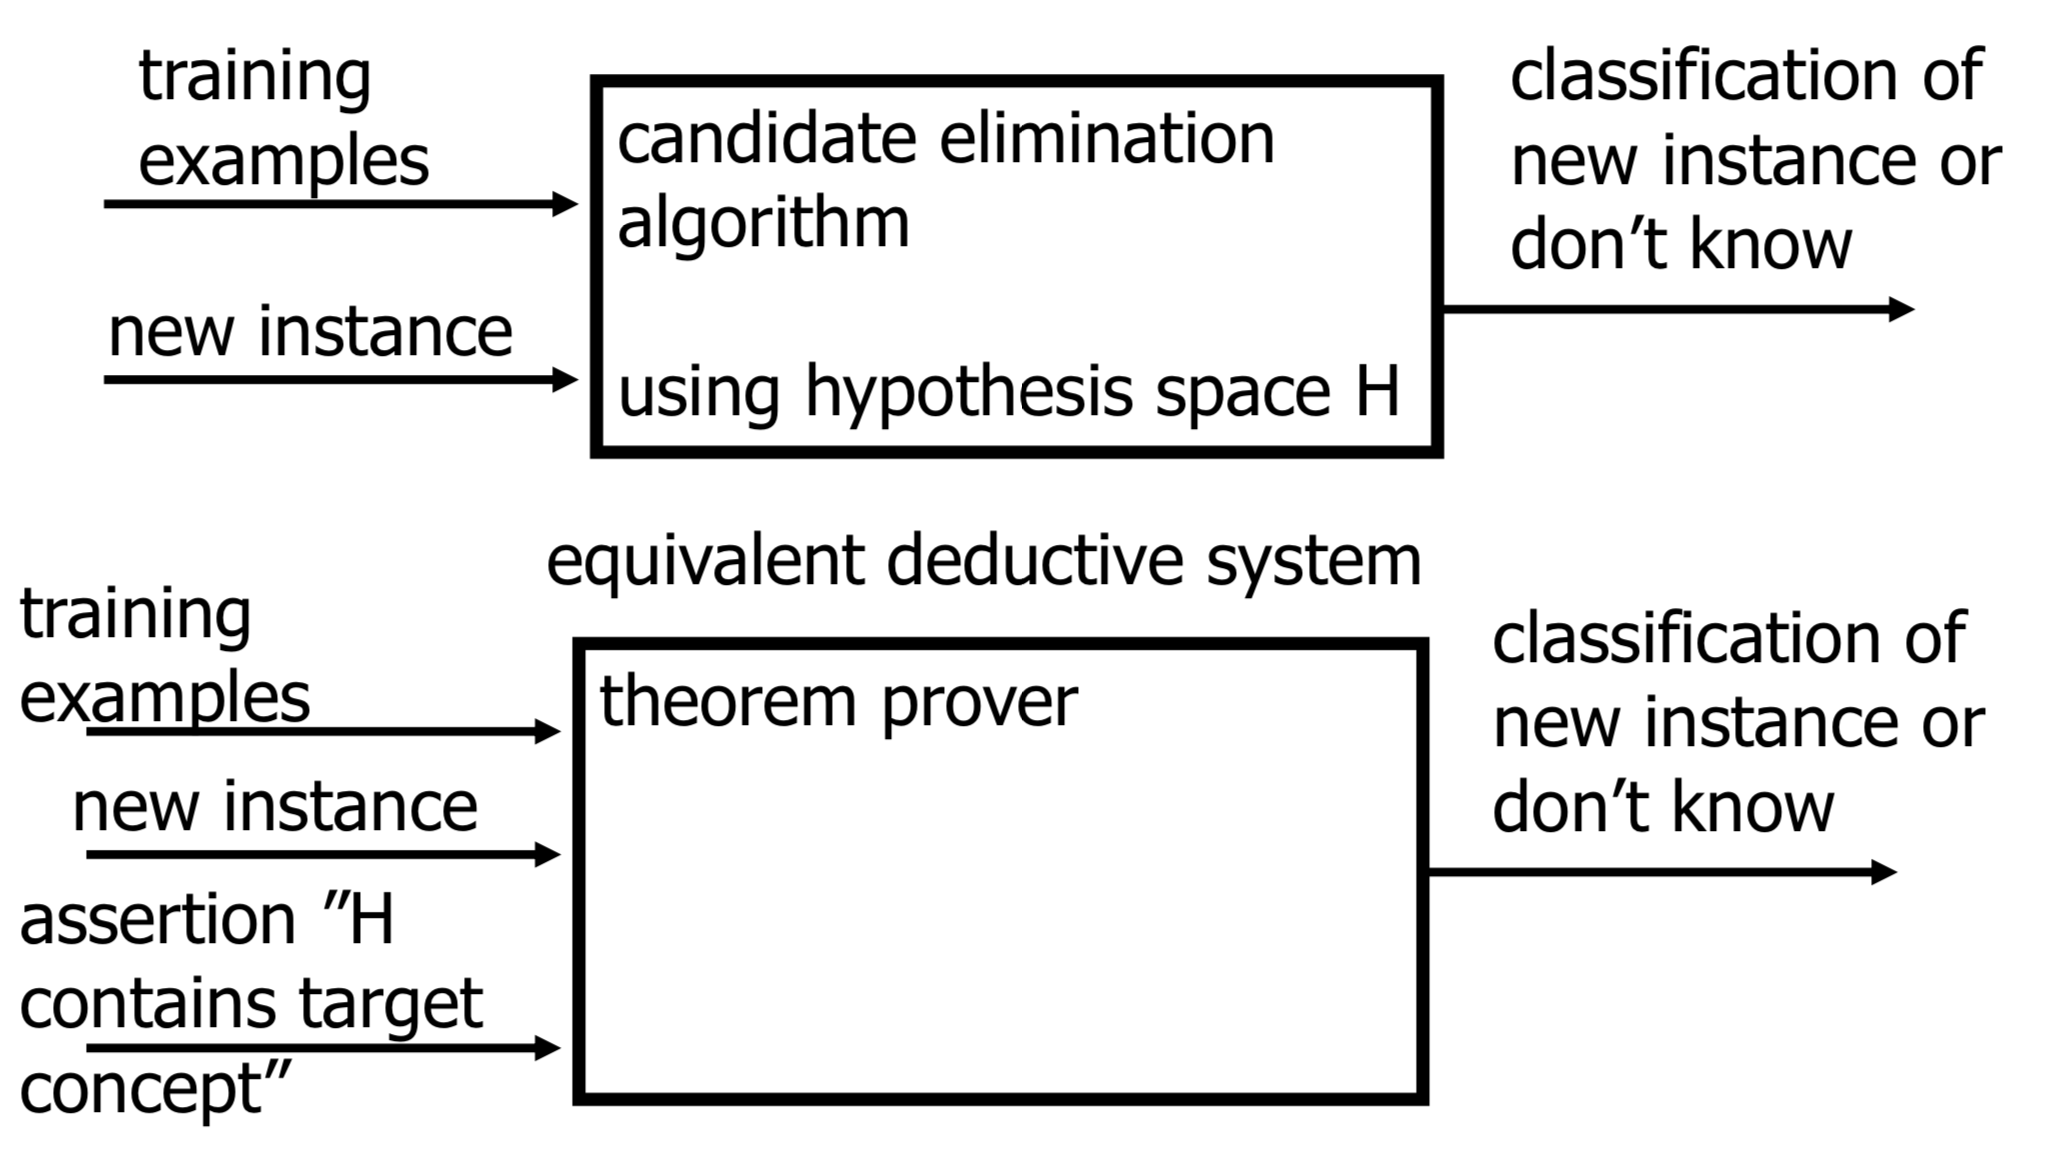
\includegraphics[scale=0.4]{Images/sistemiinduttdedutt.png}
\end{figure}
Il comportamento input-output dell'algoritmo Candidate Elimination usando uno spazio delle ipotesi H è lo stesso di un sistema deduttivo in cui diamo come input l'asserzione "H contiene il concetto target". Questa asserzione è chiamata Bias Induttivo dell'algoritmo. \newline
Il Bias è l'insieme delle asserzioni che ci permette di trasformare il problema da induttivo a deduttivo.
\subsection{Tre (algoritmi) sistemi di apprendimento con Bias differenti}
\begin{enumerate}
    \item Rote Learner: (lookup table) L'apprendimento corrisponde semplicemente alla memorizzazione di ogni esempio di allenamento osservato nella memoria. Le istanze successive vengono classificate osservandole nella memoria. Se l'istanza viene trovata in memoria, viene restituita la classificazione memorizzata. In caso contrario, il sistema rifiuta di classificare la nuova istanza. In poche parole salva gli esempi, classifica x se e solo se si "accoppiano" con uno degli esempi visti precedentemente. \newline 
    Non c'è Bias Induttivo $\rightarrow$ nessuna generalizzazione
    \item Candidate Elimination: Le nuove istanze vengono classificate solo nel caso in cui tutti i membri del Version Space corrente concordino la classificazione. In caso contrario, il sistema rifiuta di classificare la nuova istanza. \newline 
    Bias Induttivo $\rightarrow$ il concetto target può essere rappresentato nel suo spazio di ipotesi. 
    \item Find-S: Questo algoritmo, descritto in precedenza, trova l'ipotesi più specifica coerente con gli esempi di addestramento. Quindi utilizza questa ipotesi per classificare tutte le istanze successive. \newline
    Bias Induttivo $\rightarrow$ il concetto target può essere rappresentato nel suo spazio delle ipotesi e tutte le istanze sono istanze negative a meno che l'opposto non sia implicato da altre sue conoscenze.
\end{enumerate}
\clearpage

\section{Modelli Lineari}
Abbiamo visto che lo spazio delle ipotesi H costituisce l’insieme delle funzioni che possono essere realizzate dal sistema di apprendimento. Si assume che la funzione da apprendere f possa essere rappresentata da una ipotesi h in H (selezione di h attraverso i dati di apprendimento) o che almeno una ipotesi h in H sia simile a f (approssimazione). Abbiamo compreso che un Algoritmo di Ricerca nello Spazio delle Ipotesi é rappresentato in ML tramite un algoritmo di apprendimento (ad esempio adattamento dei parametri liberi del modello al task). NOTA: H non può coincidere con l’insieme di tutte le funzioni possibili ma la ricerca deve essere esaustiva $\rightarrow$ Bias Induttivo. \newline
Sia la regressione che la classificazione (quest'ultima vista nel Concept Learning) appartengono alla categoria delle tecniche di Supervised Learning, ovvero un tipo di apprendimento che fornisce a priori una serie di dati e informazioni al sistema, prima che questo cominci ad apprendere. Andremo a vedere come i Modelli lineare possono essere usati sia per la regressione (Regressione lineare) sia per la classificazione. La regressione lineare si differenzia nettamente dalla classificazione, poiché la classificazione si limita a discriminare gli elementi in un determinato numero di classi, mentre nella regressione l’input è un dato e il sistema ci restituisce un output reale approssimando una funzione. La regressione è un processo statistico che cerca di stabilire una relazione tra due o più variabili. Fornendo a un modello di regressione un valore x, questo restituirà il corrispondente valore y generato dall'elaborazione di x.

\subsection{Esempio di regressione}
La regressione come abbiamo detto é un processo di stima di una funzione a valori reali sulla base di una serie finita di campioni "rumorosi" (conosciamo le coppie (x , f(x)+random noise).
\begin{figure}[H]
    \centering
    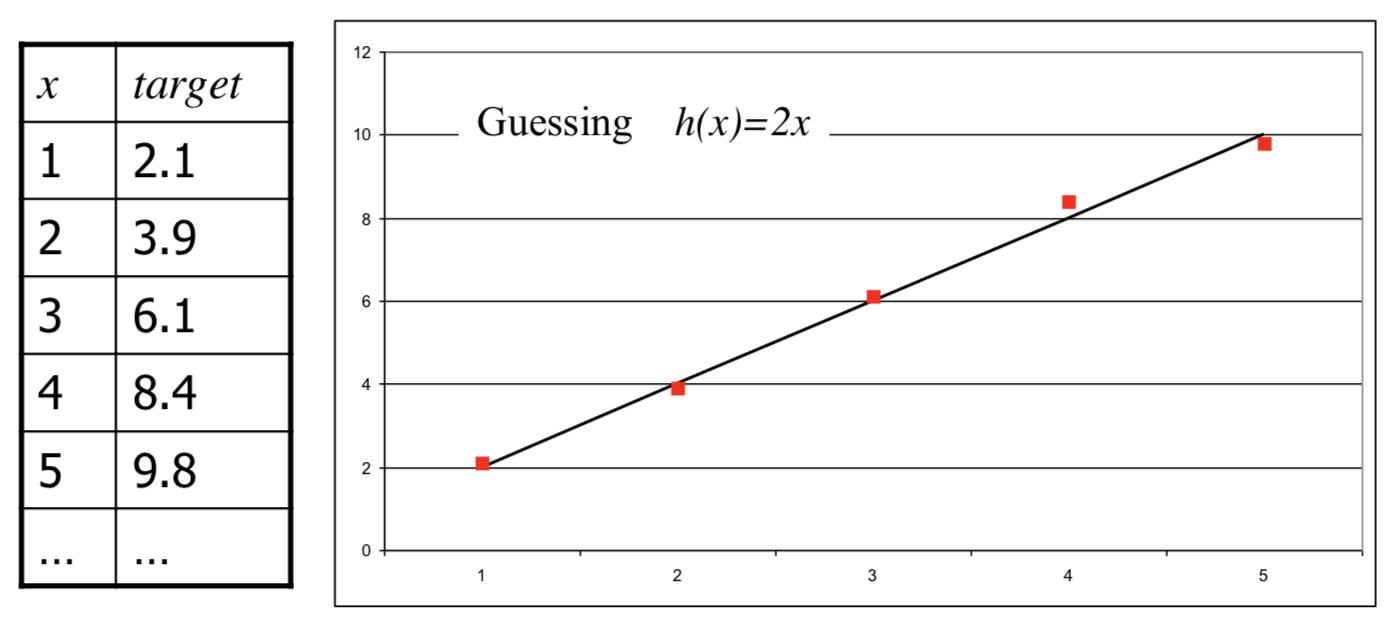
\includegraphics[scale=0.4]{Images/esempioregressione.png}
\end{figure}

\subsection{Modello di Regressione Lineare Semplice (Univariata)}
\begin{quote}
    Si parte con una variabile input x e una in output y, assumiamo il modello $h_w(x)$ espresso come $y=w_1x+w_0$ dove $w_0$ e $w_1$ sono parametri liberi a valori reali da apprendere. Usiamo la lettera w perché immaginiamo questi coefficienti come weights (pesi) poiché il valore y cambia in base a questi valori. Come si può intuire cerchiamo di adattarci ai dati con una linea retta.
\end{quote}
Lavoriamo in uno spazio di ipotesi infinite (i valori $w_i$ sono continui) ma abbiamo una buona soluzione grazie alla matematica classica. Gauss dimostró che se i valori y hanno del "rumore" distribuito allora i valori $w_1$ e $w_2$ possono essere trovati minimizzando la sommma dei quadrati degli errori (dopo vedremo meglio cosa significa). \newline
Assumiamo che la variabile y sia (linearmente) correlata a un'altra variabile x o ad altre variabili per cui $y = w_1x + w_0 + noise$, dove i $w_i$ sono i parametri liberi. Il "noise" è l'errore nella misurazione dei valori target con distribuzione normale. Cerchiamo di costruire un modello (trovare le variabili $w_i$) per predire/stimare la y per dei valori x non visti precedentemente.
\begin{figure}[H]
    \centering
    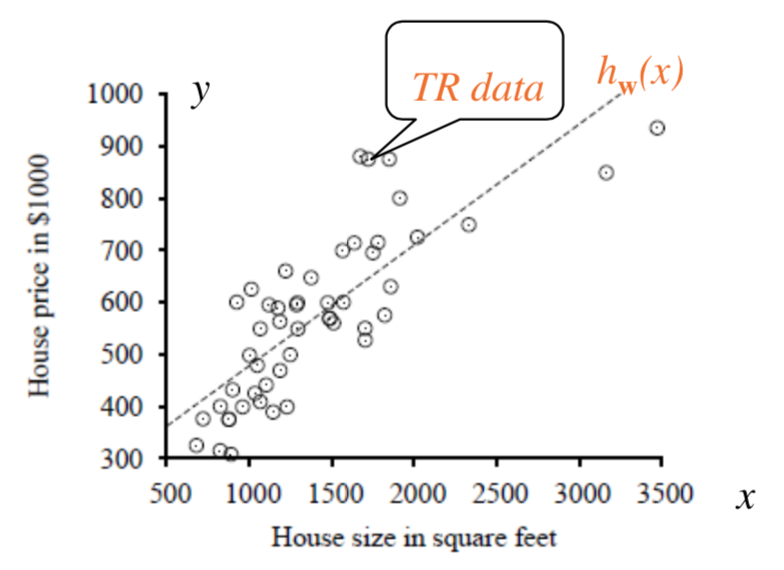
\includegraphics[scale=0.5]{Images/regresslincase1.png}
\end{figure}
Un esempio di regressione lineare per il problema sovrastante (bisogna associare il prezzo delle case in base alla metratura. y costo della casa, x metratura) é la funzione $h_w(x)=0.232*x+246$ ma come arrivare a questa funzione?

\subsection{Costruzione della funzione via LMS}
L'algoritmo LeastMeanSquare consiste nel trovare i $w_i$ per cui l'errore é minimizzato (miglior adattamento dei dati sul training set con $l$ esempi).
\begin{itemize}
    \item Dato un insieme di $l$ esempi di allenamento salvati come coppie ($x_p,y_p$)
    \item Trovare $h_w(x)=w_1x+w_0$ che minimizza l'errore medio sul Training Set
    \item Per calcolare la funzione di errore Loss usiamo la somma dei quadrati delle differenze tra il valore dato dall'esempio $y_p$ e il valore calcolato dalla funzione $h_w(x)$. Il quadrato serve per avere solo valori positivi (si potrebbe anche usare il valore assoluto, ma è meglio di no, e il perché lo vedremo in seguito)
    \begin{equation}
        Loss(h_w) = E(w) = \sum_{p = 1}^l (y_p - h_w(x_p))^2 = \sum_{p = 1}^l (y_p - (w_1*x_p + w_0))^2
    \end{equation} 
    dove $x_p$ é il p-esimo input e $y_p$ é il p-esimo output dell'esempio p. Dividendo per l ottengo la media.
\end{itemize}
Quindi dobbiamo trovare l'argomento minimo w tale che l'errore è minimo in L2 (norma 2, le norme inducono una distanza): $w = argmin_wLoss(h_w) = argmin_wE(w) \text{ in L2}$. A livello grafico lo rappresentiamo così: 
\begin{figure}[H]
    \centering
    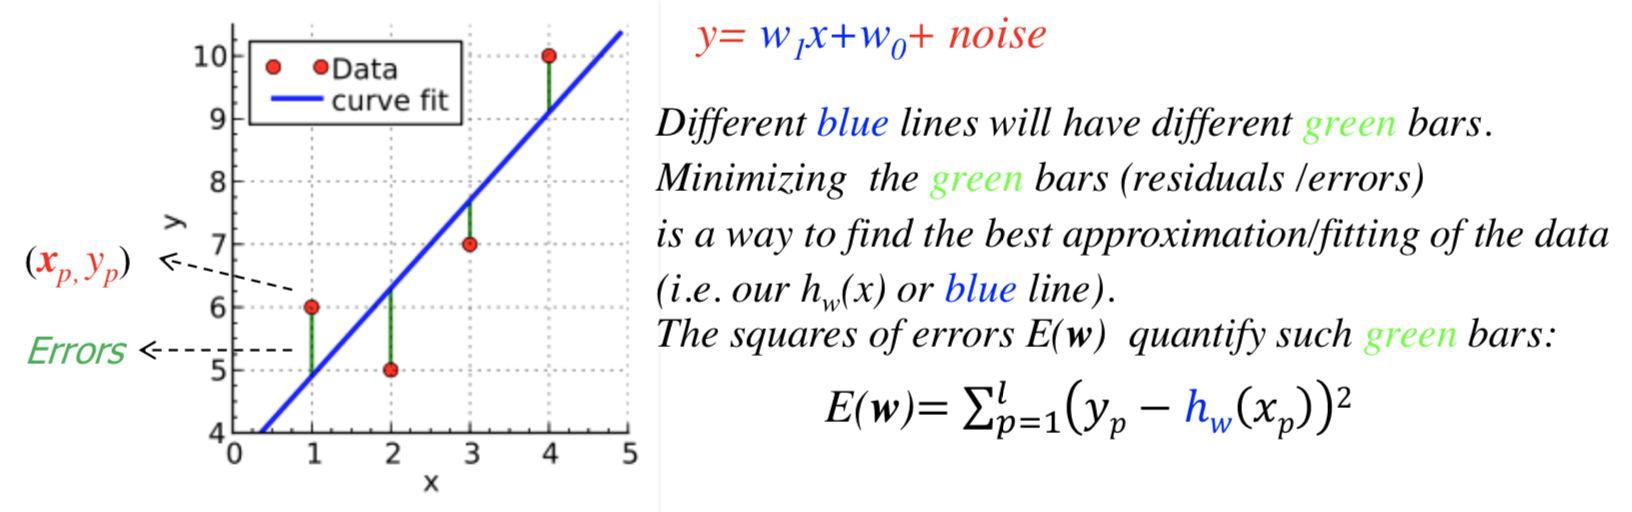
\includegraphics[scale=0.45]{Images/lmsgrafico.png}
\end{figure}
Il metodo dei minimi quadrati è un approccio standard alla soluzione approssimata di sistemi sovra-determinati, ovvero insiemi di equazioni in cui vi sono più equazioni che incognite. \newline
Il minimo locale é un punto stazionario dove il gradiente é nullo.
\begin{equation}
    \frac{\partial E(w)}{\partial w_i} = 0 \quad \text{per i = 0....dimensione\_spazio}
\end{equation}
per la regressione lineare semplice abbiamo che la funzione di Loss é minimizzata quando le sue derivate parziali rispetto a $w_0$ e $w_1$ sono 0:
\begin{equation}
    \frac{\partial E(x)}{\partial w_0} = 0 \quad \frac{\partial E(x)}{\partial w_1} = 0
\end{equation}
Se la funzione di perdita é convessa abbiamo la seguente soluzione diretta poiché non abbiamo nessun minimo locale. 
\begin{figure}[H]
    \centering
    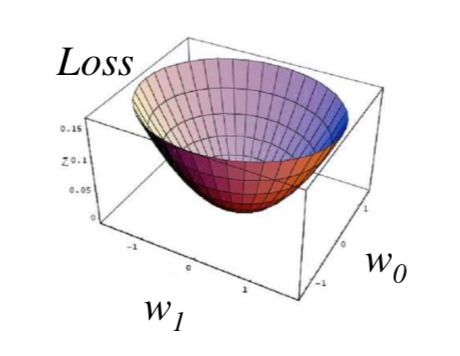
\includegraphics[scale=0.8]{Images/convexlocalmin.png}
\end{figure}
per $w_1$ abbiamo che
\begin{equation}
    w_1 = \frac{l * (\sum x_py_p) - (\sum x_p) (\sum y_p)}{l * (\sum x_p^2) - (\sum x_p)^2}
\end{equation}
mentre per $w_0$
\begin{equation}
    w_0 = \frac{\sum y_p - w_1 * \sum x_p}{l}
\end{equation}
Un approccio differente serve invece per quelle equazioni per cui il minimo della funzione di Loss spesso non ha una soluzione definita: infatti useremo una sorta di Hill Climbing iterativo che segue il gradiente discendente. Sfruttiamo le seguenti regole delle derivate parziali:
\begin{equation}
   \frac{\partial}{\partial w}k = 0 \quad \frac{\partial}{\partial w}w = 1 \quad \frac{\partial}{\partial w^2}w = 2w \quad \frac{\partial (f(w))^2}{\partial w} = 2f(w) \frac{\partial f(w)}{\partial w}
\end{equation}

ora cerchiamo il gradiente

\begin{equation}
    \frac{\partial E(w)}{\partial w_i} = \frac{\partial}{\partial w_i} (y - h_w(x))^2 =  2(y - h_w(x)) \frac{\partial}{\partial w_i} (y - h_w(x)) = 2(y - h_w(x))\frac{\partial}{\partial w_i}(y - (w_1x+w_0))
\end{equation}

applicando $w_0$ e $w_1$ nella derivata ottengo due equazioni

\begin{equation}
    \frac{\partial E(w)}{\partial w_0} = -2(y - h_w(x)) \quad e \quad \frac{\partial E(w)}{\partial w_1} = -2(y - h_w(x)) * x
\end{equation}

\begin{figure}[H]
    \centering
    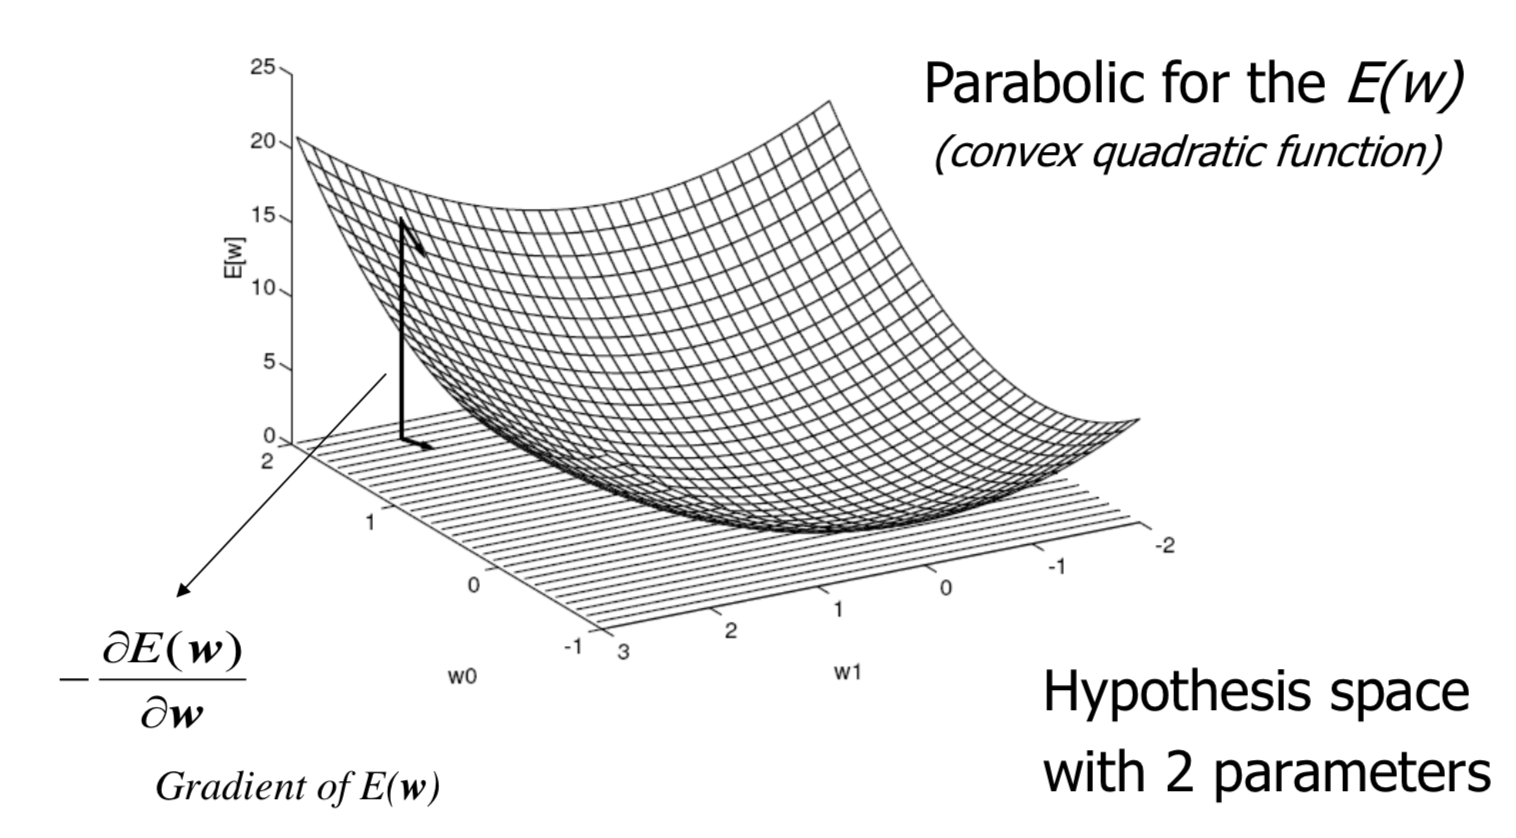
\includegraphics[scale=0.4]{Images/gradientlinearspace.png}
\end{figure}

\subsubsection{Gradiente discendente}
La derivazione precedente suggerisce la costruzione di un algoritmo iterativo basato su $\partial E(w) / \partial w_i$. Il gradiente ci indica la direzione di salita, possiamo spostarci verso il minimo con discesa del gradiente $\Delta w = - gradienteE(w)$. La ricerca locale inizia con il vettore che contiene i valori dei pesi, viene modificato iterativamente per diminuire fino a minimizzare l'errore della funzione.
\begin{quote}
    $w_{new} = w_{old} + \eta * \Delta w$ dove $\eta$ é una costante che indicare il rateo di apprendimento
\end{quote}
\begin{figure}[H]
    \centering
    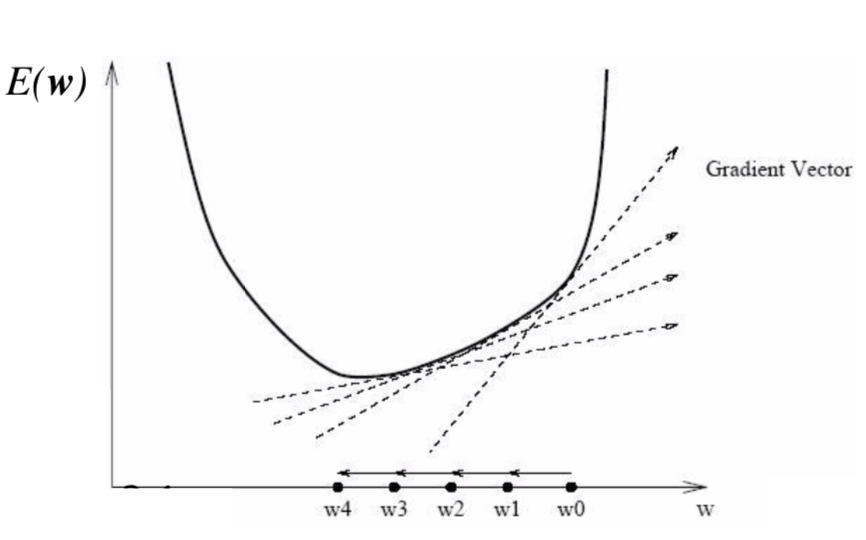
\includegraphics[scale=0.5]{Images/gradientvector.png}
\end{figure}

Le nostre regole di correzione dell'errore (chiamate delta-rule) cambiano i valori w proporzionalmente all'errore:
\begin{equation}
    \Delta w_0 = - \frac{\partial E(w)}{\partial w_0} = 2(y - h_w(x)) \quad e \quad \Delta w_1 = - \frac{\partial E(w)}{\partial w_1} = 2(y - h_w(x)) * x
\end{equation}


\begin{itemize}
    \item se $(y_{target}-output)=0$ significa che non abbiamo errore e quindi nessuna correzione da fare
    \item se $(output>y_{target})$ cioè $(y-h)<0$ vuol dire che l'output trovato é troppo alto quindi:
        \begin{itemize}
            \item $\Delta w_0$ negativo $\rightarrow$ riduco $w_0$
            \item se $(x_{input}>0$ e $\Delta w_1$ negativo $\rightarrow$ riduco $w_1$ altrimenti incremento $w_1$
        \end{itemize}
    \item se $(output<y_{target})$ cioè $(y-h)>0$ vuol dire che l'output trovato é troppo basso quindi: %non sono sicuro su questa parte
        \begin{itemize}
            \item $\Delta w_0$ negativo $\rightarrow$ aumento $w_0$
            \item se $(x_{input}<0$ e $\Delta w_1$ positivo $\rightarrow$ aumento $w_1$ altrimenti diminuisco $w_1$
        \end{itemize}
\end{itemize}
Questo ci permette la ricerca in uno spazio delle ipotesi infinito, e può essere applicato facilmente per spazi H continui e con funzione di Loss differenziabile (altrimenti non posso calcolare il gradiente!). Per questo motivo il valore assoluto è scomodo: potrebbe rendere non differenziabile la funzione. \newline
Arriviamo quindi a definire le funzioni su $l$  esempi:
\begin{equation}
    \Delta w_0 = - \frac{\partial E(w)}{\partial w_0} = 2 \sum_{p=0}^l (y_p - h_w(x_p)) \quad e \quad \Delta w_1 = - \frac{\partial E(w)}{\partial w_1} = 2 \sum_{p=0}^l (y_p - h_w(x_p)) * x_p
\end{equation}
Ora può venirci in mente una domanda, aggiorniamo i $w_i$ dopo aver ispezionato un insieme di esempi di allenamento l, oppure dopo ogni singolo esempio analizzato?
\begin{itemize}
    \item Batch Algorithm: calcoliamo la sommatoria dell'errore quadratico su l pattern diversi e otteniamo il gradiente, dopo l dati di training sommati abbiamo una “epoca” e aggiorniamo i $w_i$. Puó essere molto lento...
    \item On-Line Algorithm: calcoliamo il gradiente su un pattern p e poi aggiorniamo subito $w_i$. Solitamente é piú veloce del Batch...
\end{itemize}

\subsection{Modello di Regressione Lineare Multivariato}
Il caso standard é con due variabili, ma in realtà possiamo avere in input centinaia di variabili, l'esempio sul prezzo delle case in realtà conteneva anche le variabili che indicavano il numero delle stanze, l'età della casa ecc... 
\subsubsection{Notazione dei dati}
\begin{figure}[H]
    \centering
    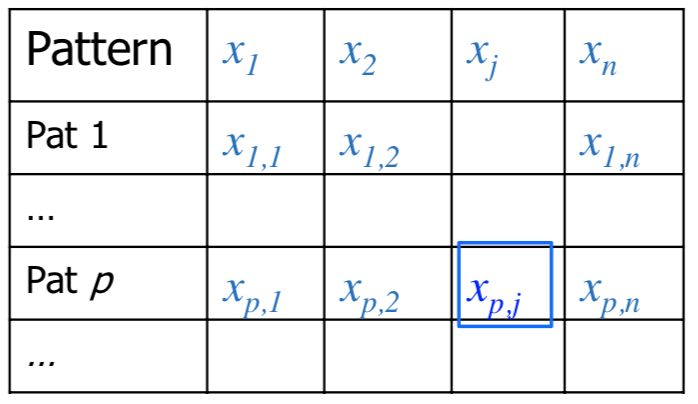
\includegraphics[scale=0.6]{Images/datanotation.png}
\end{figure}
X é una matrice $l$ righe * $n$ colonne (numero di pattern * numero di variabili), ogni riga della matrice $X_i$ é un vettore che rappresenta un esempio. $x_{i,j}$ é uno scalare cioè la componente j della riga i. \newline
Stiamo quindi dicendo che ogni esempio $x_p$ é un vettore di n elementi. \newline
Supponendo vettori colonna x e w, con numero di esempi $l$ e dimensione in input n, possiamo scrivere 
\begin{equation}
    w^Tx+w_0 = w_0+w_1x_1+w_2x_2+...+w_nx_n
\end{equation} 
dove $w_0$ é il bias (non c'entra con il Concept Learning) é la distanza dalla componente 0. Possiamo anche scrivere che $x_0=1$ in modo tale da poter scrivere che $w^Tx = x^Tw$ quindi: $x^T = [1,x_1,...,x_n]$ e $w^T = [w_0, w_1, ..., w_n]$
\clearpage

\subsection{Hyperplane}
Anziché adattare una retta, adattiamo un iperpiano. 
\begin{figure}[H]
    \centering
    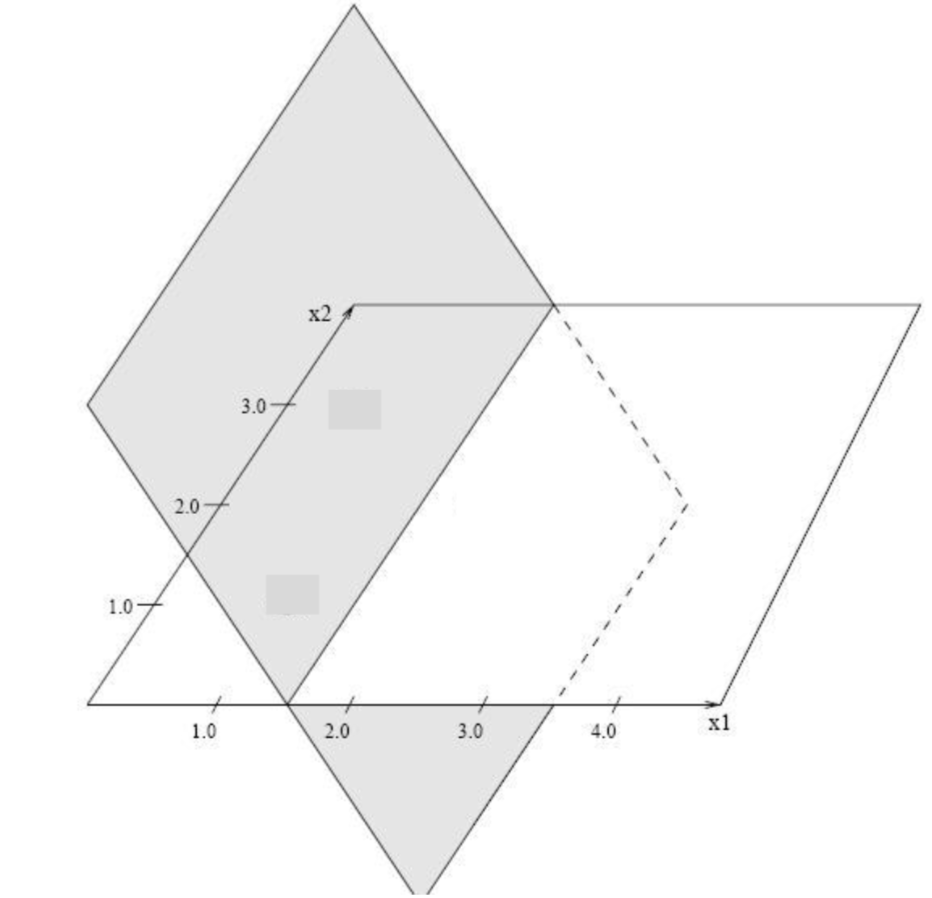
\includegraphics[scale=0.4]{Images/iperpiano.png}
\end{figure}
quindi abbiamo che $w^Tx = w_1x_1 + w_2x_2 + w_0$ e $h(x_p) = x_p^Tw=\sum_{i = 0}^n x_{p,i} w_i$
dove $x_{p,i}$ é la componente i-esima del p-esimo esempio.

\subsection{Gradiente Discendente Algoritmo}
\begin{enumerate}
    \item si inizia con il vettore dei pesi $w_{iniziale}$ e si fissa un $0<\eta <1$
    \item si calcola il gradiente $\Delta w = -gradienteE(w) = -(\partial E(w) / \partial w)$
    \item si calcola $w_{new} = w_{old} + \eta * \Delta w$
    \item ripetere dal passo 2 finché E(w) é sufficientemente piccolo
\end{enumerate}
La versione batch dell'algoritmo si occupa di calcolare $\Delta w$ dopo un insieme di esempi l. La versione online invece aggiorna $\Delta w$ dopo ogni esempio p al posto di aspettare la sommatoria su l, ma ha bisogno di uno step size $\eta$ più piccolo. 

\begin{figure}[H]
    \centering
    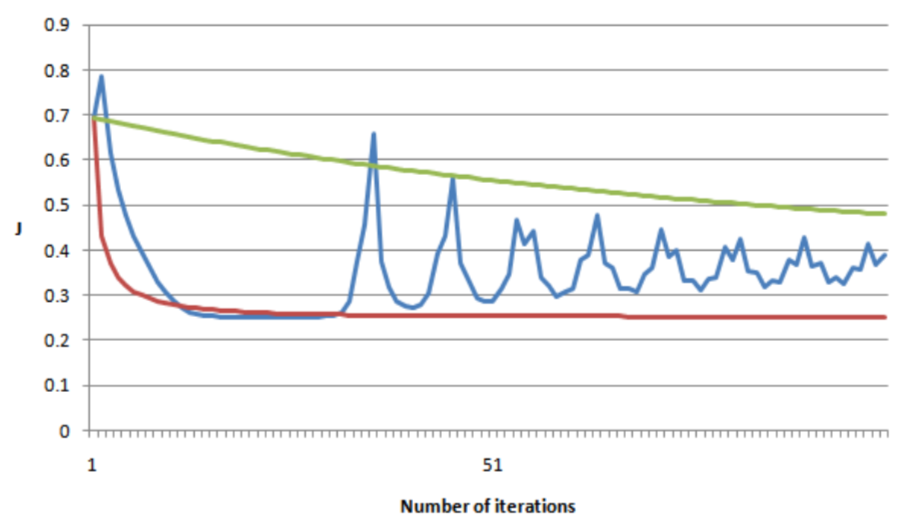
\includegraphics[scale=0.6]{Images/examplegraphloss.png}
\end{figure}

Questi sono tre esempi di curve, dove noi andremo a preferire quella che diminuisce nel minor tempo possibile (quella che impiega meno iterazioni). 

\subsection{Vantaggi dei modelli lineari}
Se funziona bene è un modello "meraviglioso", molto semplice dove tutte le informazioni sui dati sono contenute nel vettore w. Facile da interpretare tant'è che viene usato in medicina, biologia, chimica, economia... Una delle cose fondamentali é che sono ammessi dati rumorosi e viene usato/incluso in modelli più complessi.

\subsection{Limitazioni}
La regressione lineare presenta delle limitazioni quando si parla di problemi non lineari.

\begin{figure}[H]
    \centering
    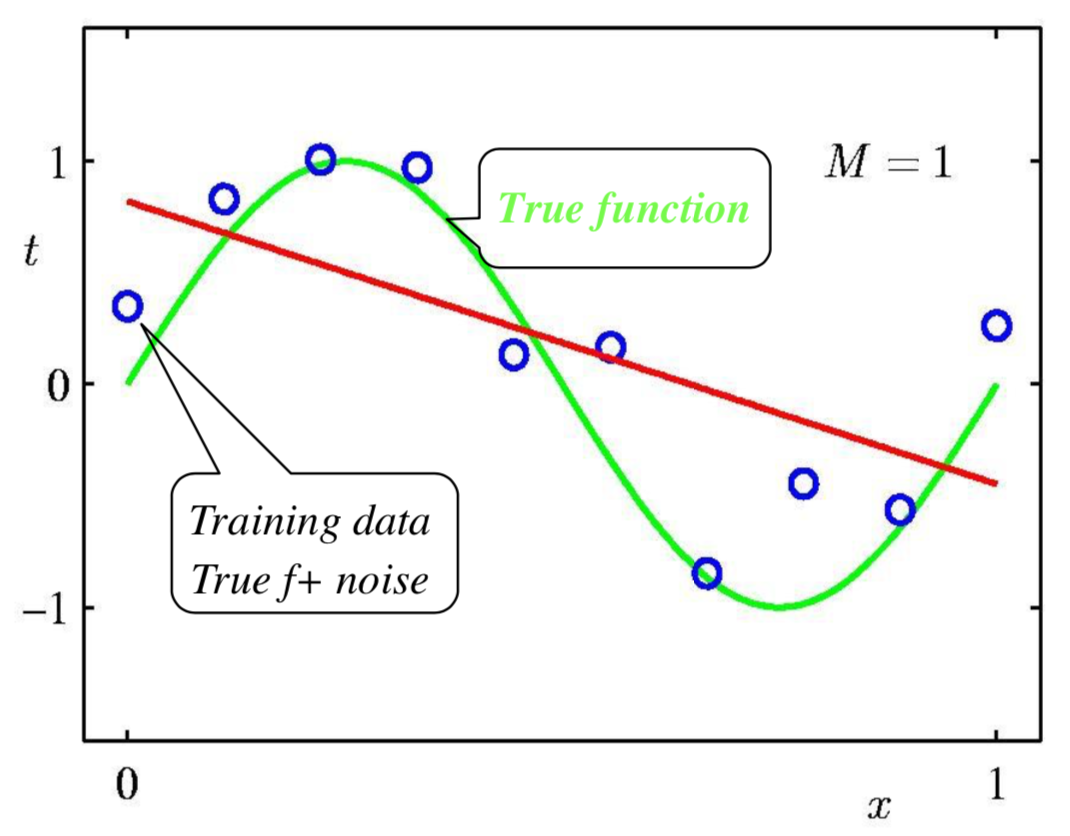
\includegraphics[scale=0.35]{Images/linearnonlinear.png}
\end{figure}

Notiamo che $h_w(X)=w_1x+w_0$ definita "lineare" non significa che é una linea retta, ma piuttosto come il modo in cui i coefficienti w occorrono nell'equazione di regressione (cioè lineare in w, non in x). Quindi, possiamo anche trasformare gli input, come $x,x^2,x^3,...$ con relazioni non lineari tra input e output. Sfruttando l'algoritmo LMS utilizzato fino ad ora:
\begin{equation}
    y(x,w) = w_0+w_1x+w_2x^2+...+w_Mx^M=\sum_{j = 0}^M w_jx^j
\end{equation}

\subsubsection{Esempio}
Rispetto all'equazione scritta precedenete in questo caso abbiamo M=2. La funzione non deve essere lineare nell'argomento (variabili in input) ma solo nei parametri che sono determinati per dare il miglior adattamento. 
\begin{figure}[H]
    \centering
    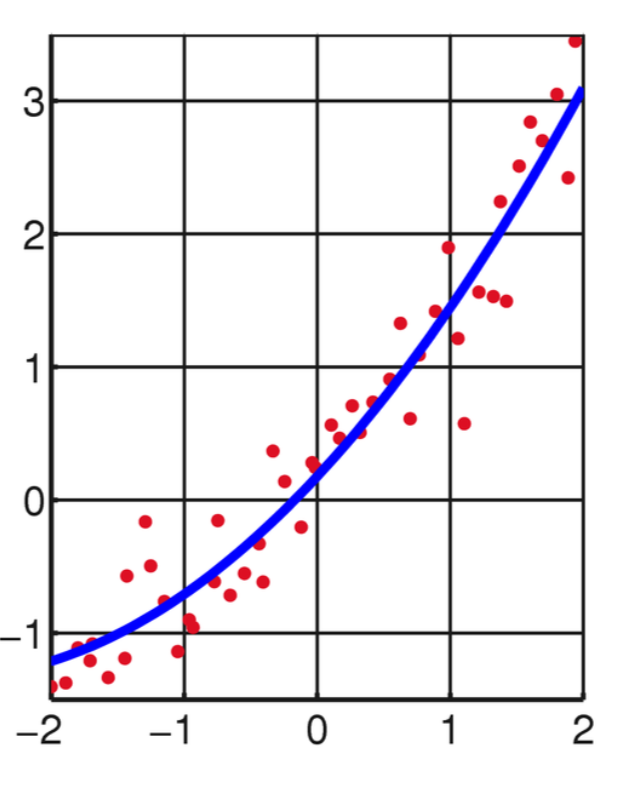
\includegraphics[scale=0.35]{Images/quadraticfit.png}
    \caption{fitting su una funzione quadratica (linea blu) attraverso un set di dati (punti rossi)}
\end{figure}

\subsection{Linear Basis Expansion}
Prima calcolavamo il prodotto scalare tra w e x (w trasposto per x) ora prendo delle trasformazioni (anche non lineari) del vettore x e le uso come un'espansione della base, combinandole in maniera lineare in accordo con la funzione $\phi_k$. 
\begin{equation}
    h_w(x)=\sum_{k=0}^K w_k \phi_k(x)
\end{equation}
La funzione $\phi$ puó essere espressa come rappresentazioni polinomiali del tipo $\phi(x)=x_j^2$ oppure $\phi(x)=x_j*x_i$, o ancora trasformazioni non lineari come $\phi(x)=log(x_j)$. Il modello é rimasto lineare nei parametri (é sempre x!) quindi possiamo usare lo stesso algoritmo di prima. 
\subsubsection{Esempi}
\begin{itemize}
    \item dimensione di x = 1 e $\phi_j(x)=x^j$ 
    \begin{equation}
    h(x) = w_0+w_1x+w_2x^2+...+w_Mx^M=\sum_{j = 0}^M w_jx^j
    \end{equation}
    regressione polinomiale ad 1 dimensione (K=M)
    \item $\phi(x)=\phi([x_1,x_2])$
    \begin{equation}
    h(x) = w_0+w_1x_1+w_2x_2+w_3x_1x_2+w_4x_1^2
    \end{equation}
\end{itemize}
Quale $\phi$ scegliere? Adottiamo un modello in stile dizionario? I punti a favore sono la maggiore espressività poiché può modellare relazioni più complesse di quelle lineari. I punti contro sono l'avere una grossa base di funzioni che richiedono metodi per controllare la complessità del modello, vediamo perché...
\begin{itemize}
    \item grado del polinomio = 1, notiamo che é esegue troppo "underfitting".
    \begin{figure}[H]
    \centering
    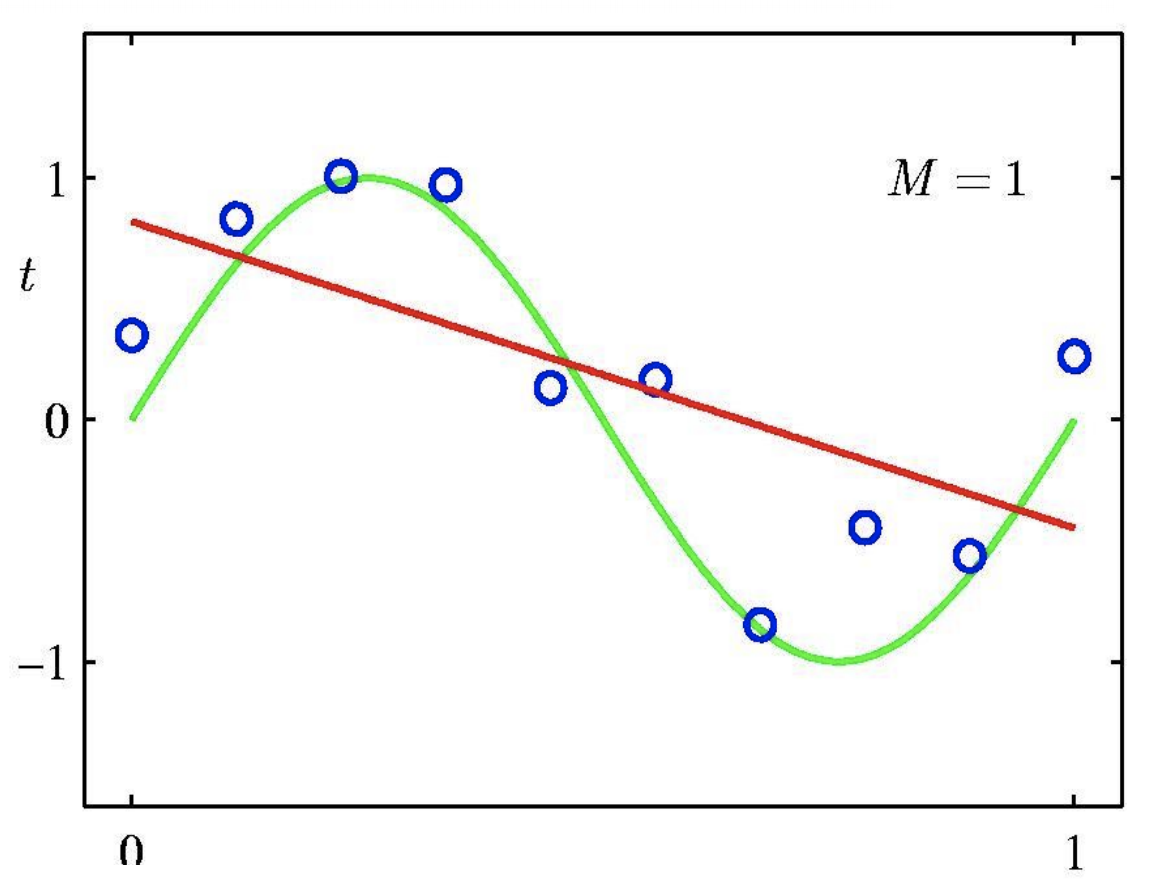
\includegraphics[scale=0.3]{Images/polgrado1underfit.png}
    \end{figure}
    \clearpage
    
    \item ordine del polinomio = 3, va bene ma potrebbe servirci più flessibilità.
    \begin{figure}[H]
    \centering
    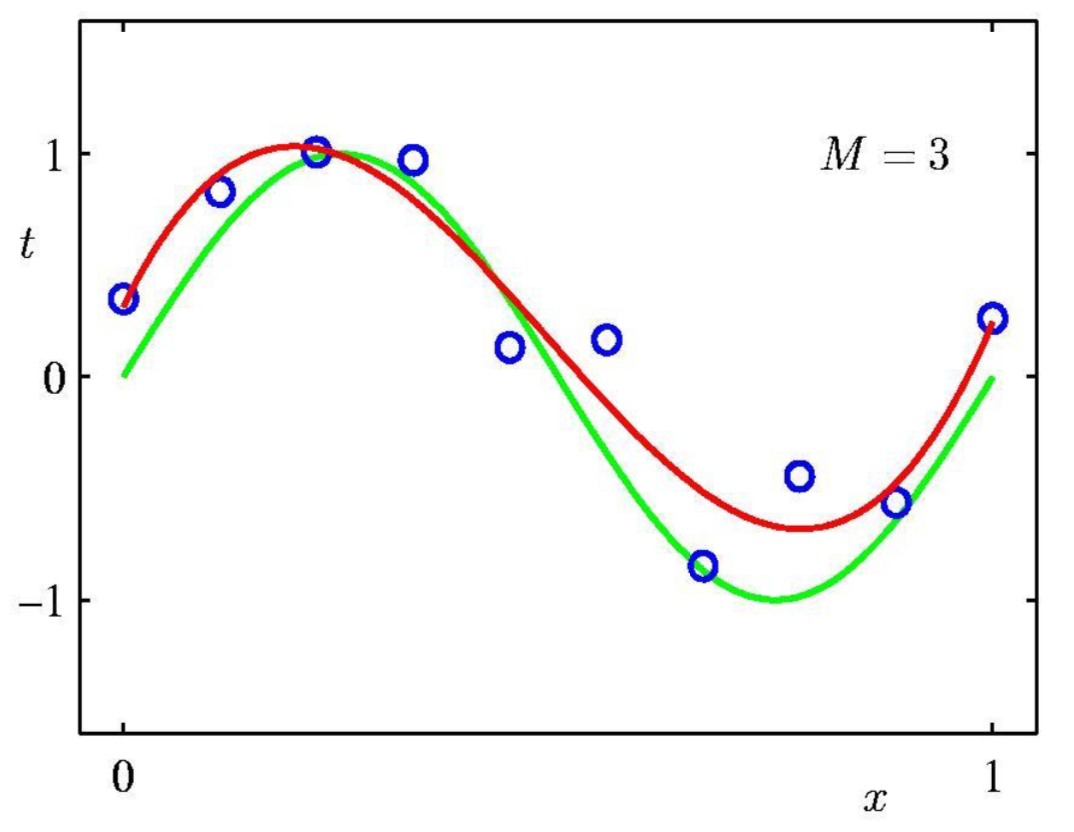
\includegraphics[scale=0.3]{Images/3gradepol.png}
    \end{figure}
    
    \item grado del polinomio = 9, notiamo che é flessibilissimo ma eccessivo. Cioè E(w)=0 ma dobbiamo tenere conto degli errori sul test set, perché se i dati fossero rumorosi noi stiamo adattando al rumore.
    \begin{figure}[H]
    \centering
    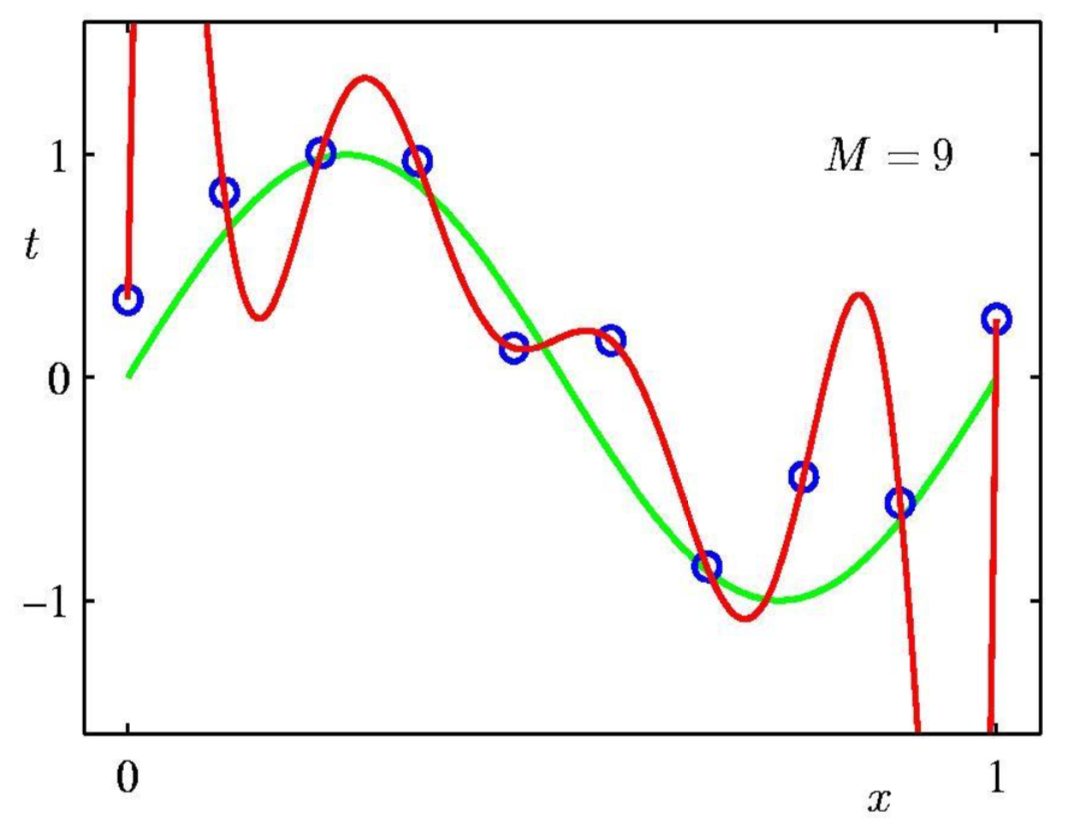
\includegraphics[scale=0.3]{Images/9gradepol.png}
    \end{figure}
\end{itemize}

\subsubsection{Tradeoff per la complessitá}
\begin{itemize}
    \item Se scegliamo un modello troppo semplice non fitta bene i dati e abbiamo una soluzione vincolata (ce ne accorgiamo perché E(w) è alto) $\rightarrow$ Underfitting
    \item Se scegliamo un modello troppo complesso siamo troppo sensibili alla piccole perturbazioni dei dati $\rightarrow$ Overfitting
\end{itemize}
Vogliamo scegliere la regolarizzazione per bilanciare bias e varianza e lo faremo attraverso il controllo della complessità del modello.
\clearpage

\subsection{Regolarizzazione - Ridge Regression}
Possiamo evitare l'overfitting penalizzando le funzioni complesse mantenendo comunque la flessibilità dello spazio delle ipotesi (un po' come il rasoio di Occam, si preferisce lo spazio delle ipotesi più semplice che fitta i dati). \newline
La Ridge Regression, chiamata anche regolarizzazione di Tikhonov, é sempre un modello LMS ma regolarizzato. Per esempio é possibile aggiungere vincoli alla sommatoria del valore di $|w_j|$ favorendo modelli "sparsi" (sono modelli con meno termini dovuti a pesi $w_j$ = 0). \newline 
Un modello non regolarizzato fitta bene ma generalizza male (non ci serve a niente). Vorrei un modello semplice (magari con alcuni coefficienti che valgono zero). Come si fa? Aggiungiamo una penalizzazione alla complessità del modello della loss, sommando la norma del vettore w, moltiplicato per un parametro $\lambda$ chiamato coefficiente di regolarizzazione. Con il parametro lambda (che é una costante), non ho più bisogno di modificare il grado dei polinomi, o analizzare funzioni più complesse.
\begin{equation}
    definito \quad E_D(w)+\lambda E_W(w) \quad otteniamo \quad Loss(h_w)=\sum_{p} (y_p-h_w(x_p))^2+\lambda ||w||^2
\end{equation}
Ottenendo quindi la nuova regola di apprendimento caratterizzata dal weight decay (aggiunta di $2\lambda w$)
\begin{equation}
    w_{new}= w_{old} + \eta*\Delta w - 2 \lambda w_{old}
\end{equation}
Per via di di $-2\lambda w_{old}$ decremento il parametro se positivo, lo incremento se negativo (in pratica lo avvicino a zero $\rightarrow$ weight decay). Quindi possiamo controllare la complessità del polinomio sfruttando solamente $\lambda$.\newline
Finora abbiamo posto tutta la complessità nel bias di linguaggio, cioè un vincolo posto sul modello (lineare, quadratico, etc). Con la regolarizzazione sposto tutto sul bias di ricerca, cioè sull'algoritmo, come l'algoritmo riesce a trovare la soluzione. Noi non poniamo a priori una complessità al modello, ma sarà il mio metodo di ricerca intelligente a scegliere la funzione più semplice.
\begin{figure}[H]
\centering
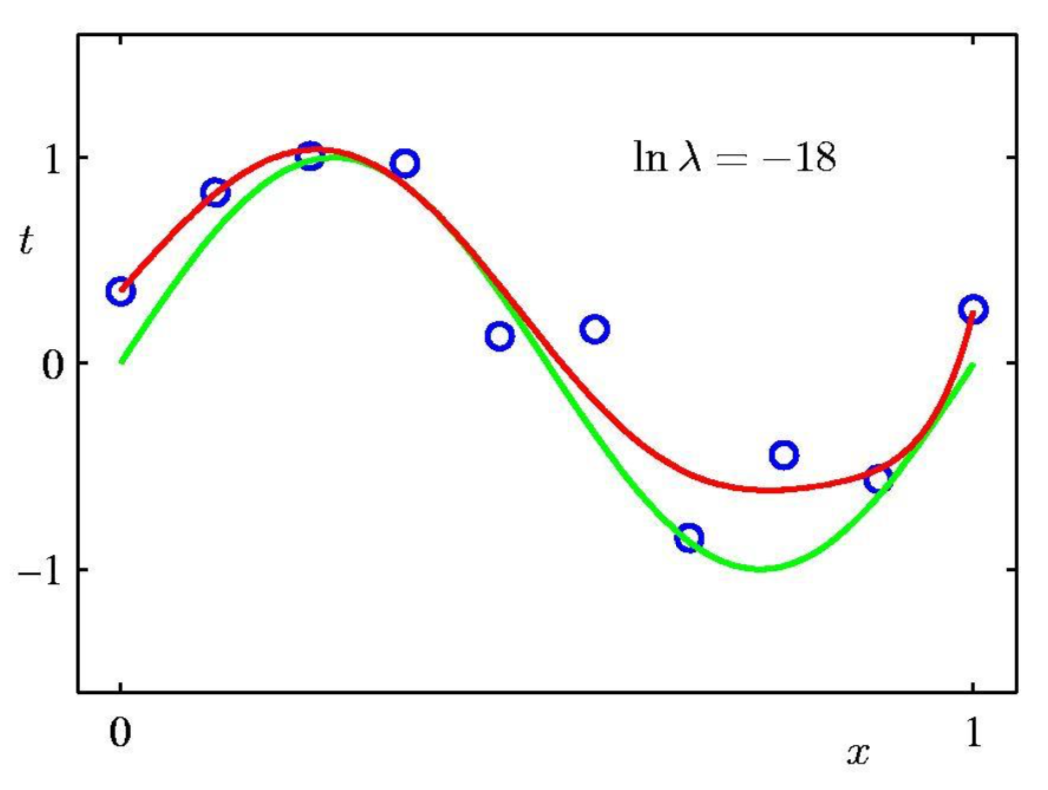
\includegraphics[scale=0.3]{Images/9gradopollambda.png}
\caption{Polinomio di grado 9 con $log_e(\lambda) = -18$ quindi $\lambda$ basso}
\end{figure}

\begin{figure}[H]
\centering
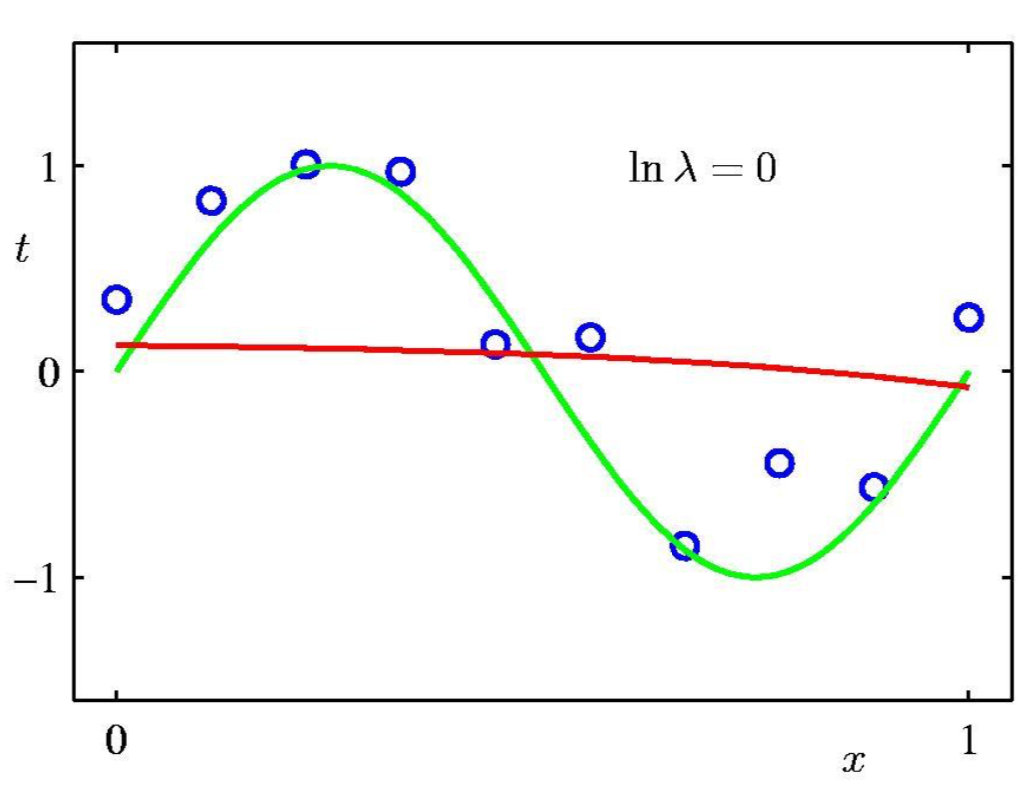
\includegraphics[scale=0.3]{Images/9gradopollambda0.png}
\caption{Polinomio di grado 9 con $log_e(\lambda) = 0$ quindi $\lambda$ tropo alto}
\end{figure}

\begin{figure}[H]
\centering
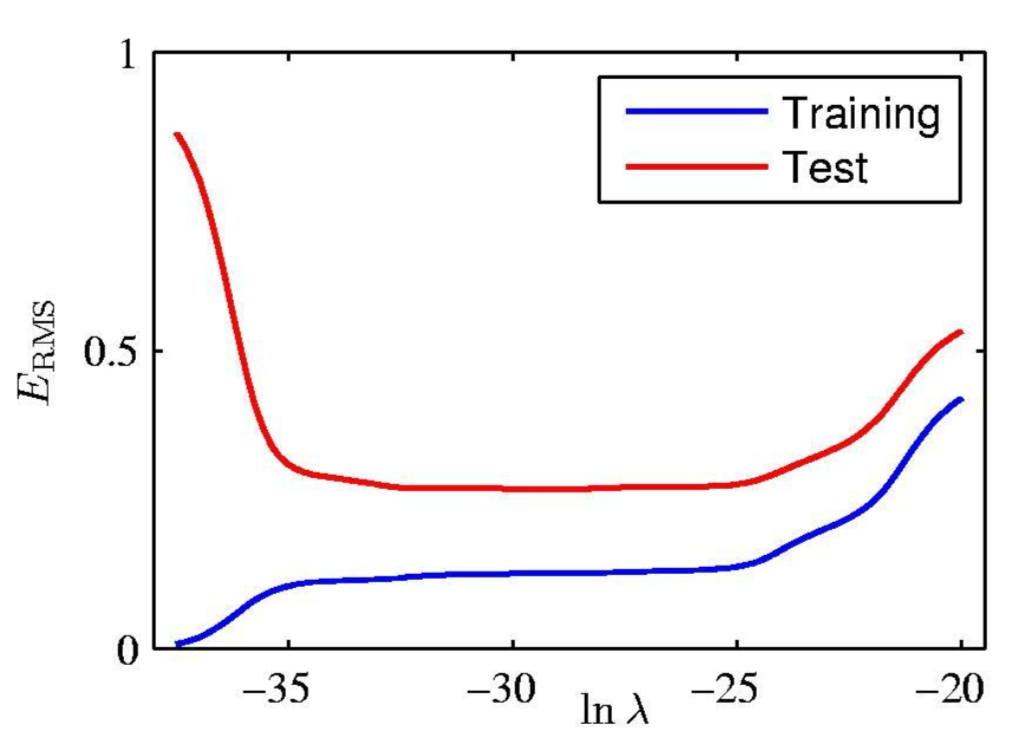
\includegraphics[scale=0.3]{Images/Ermsvslambda.png}
\caption{$E_{RMS}$ vs $log_e(\lambda)$}
\end{figure}

Possiamo concludere quindi dicendo che se $\lambda$ é basso $\rightarrow$ overfitting, mentre se $\lambda$ alto $\rightarrow$ underfitting.

\subsection{Limitazione delle funzioni a base fissa}
Quando facciamo un'espansione polinomiale, la dimensionalità del problema cresce molto, e i dati che prima erano densi, potrebbero diventare sparsi. Quando la dimensione dell'input aumenta, il problema diventa enormemente difficile (la difficoltà cresce esponenzialmente, proprio come il volume con le dimensioni). Inoltre, se inizio a mettere dati a caso, rischio di aumentare il rumore. Avere la funzione base che opera su ogni dimensione di uno spazio implica che lo spazio di input richieda un numero combinatorio di funzioni. Per esempio un polinomio dell'ordine 3, utilizza tutte le combinazioni di variabili di input dovute ai prodotti $x_1x_2, x_2x_3, ..., x_1x_2x_3 \text{ ecc... }\rightarrow D^3$ (approssimare all'aumentare di D) \newline
In altri modelli, vedremo come possiamo farcela con meno funzioni di base. Si scelgono le funzioni dal dizionario e si mettono dei parametri liberi, per adattare la $\phi$ ad H.
Ho il vantaggio di essere più generale, ma il modello diventa non lineare rispetto a w (vedremo nelle reti neurali). \newline 
In altri modelli invece di calcolare esplicitamente la $\phi$, viene fatta in maniera implicita, col concetto di funzioni kernel, controllando la complessità del modello direttamente con la funzione obiettivo, non più con una penalità aggiunta dopo (SVM).
\clearpage

\subsection{Classificazione con il modello lineare}
Possiamo utilizzare il modello lineare per la classificazione, in questo caso usiamo un iperpiano ($w^T*x$) assumendo valori positivi o negativi. Sfruttiamo questi modelli per decidere se un punto x appartiene alla zona positiva o negativa dell'iperpiano. Quindi vogliamo impostare w vettore in modo tale da ottenere una buona precisione di classificazione.

\subsubsection{Visione geometrica dell'iperpiano}
$w^T*x$ (prodotto di vettore riga per vettore colonna) definisce un iperpiano, il Decision Boundary é il luogo geometrico\footnote{é una linea, o un piano (quando ci troviamo in dimensioni più gradi)} dei punti dove l'iperpiano vale zero e può essere utilizzato per classificare.
\begin{figure}[H]
\centering
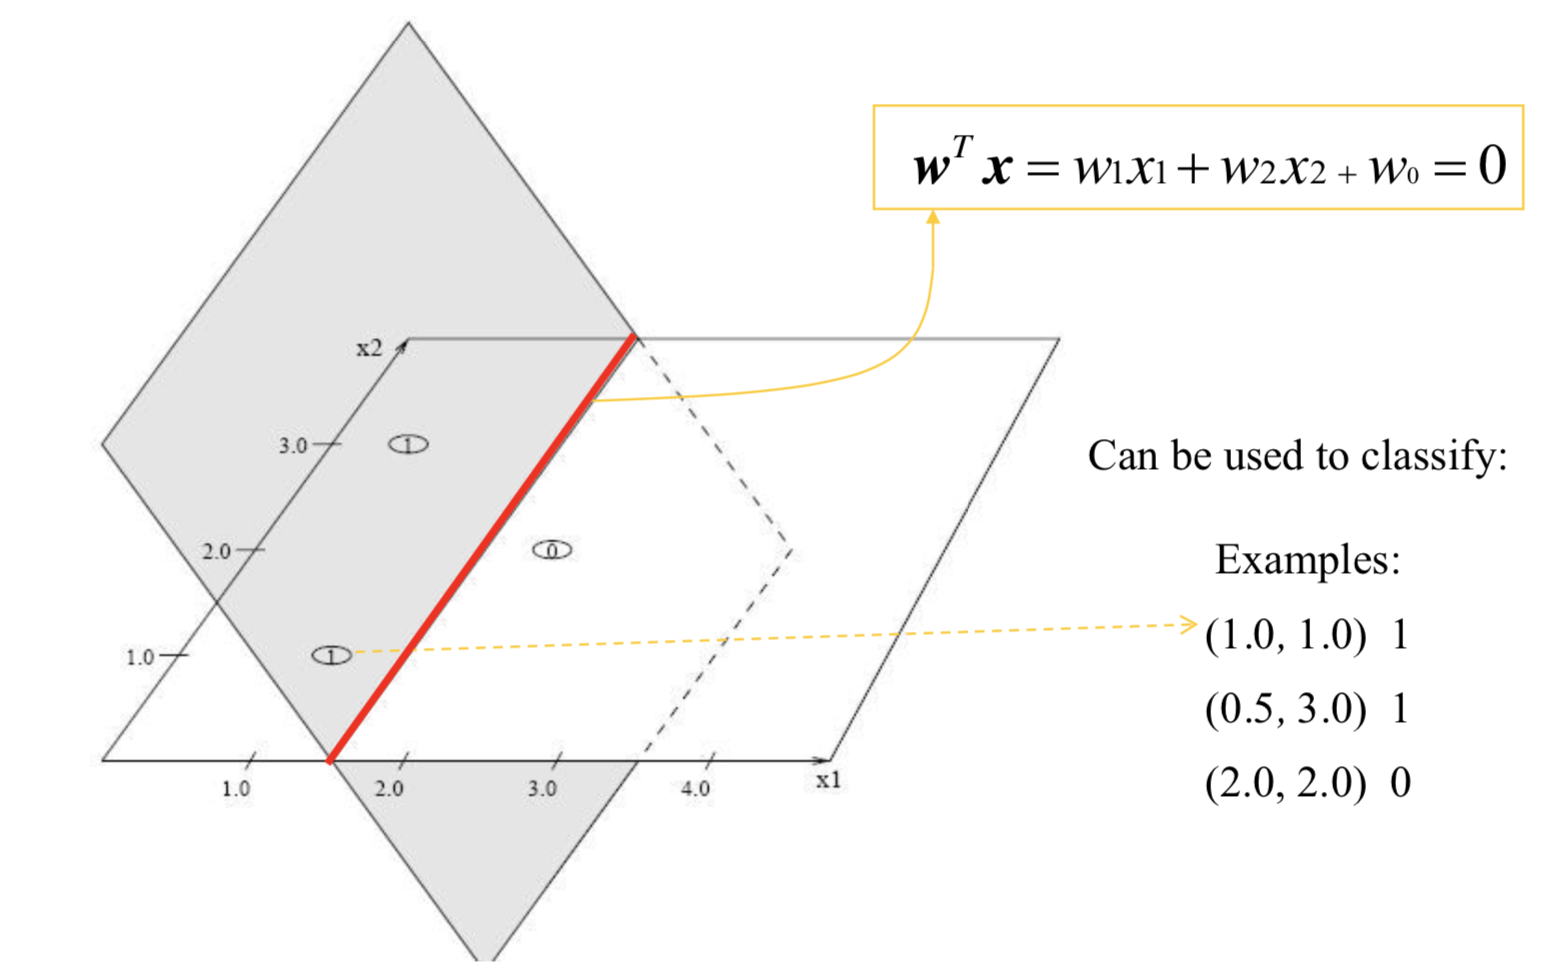
\includegraphics[scale=0.4]{Images/deecisionbundary.png}
\end{figure}
Quindi possiamo definire una funzione di classificazione del tipo:
\begin{equation}
  h(x)=\begin{cases}
    1 & \text{if $w^Tx+w_0\geq 0$}.\\
    0 & \text{altrimenti}.
  \end{cases}
\end{equation}
che possiamo scrivere come $h(x)=segno(w^Tx+w_0) \rightarrow h(x_p)=sign(x_p^Tw)=sign(\sum_{i=0}^n x_{p,i}w_i)$
\begin{figure}[H]
\centering
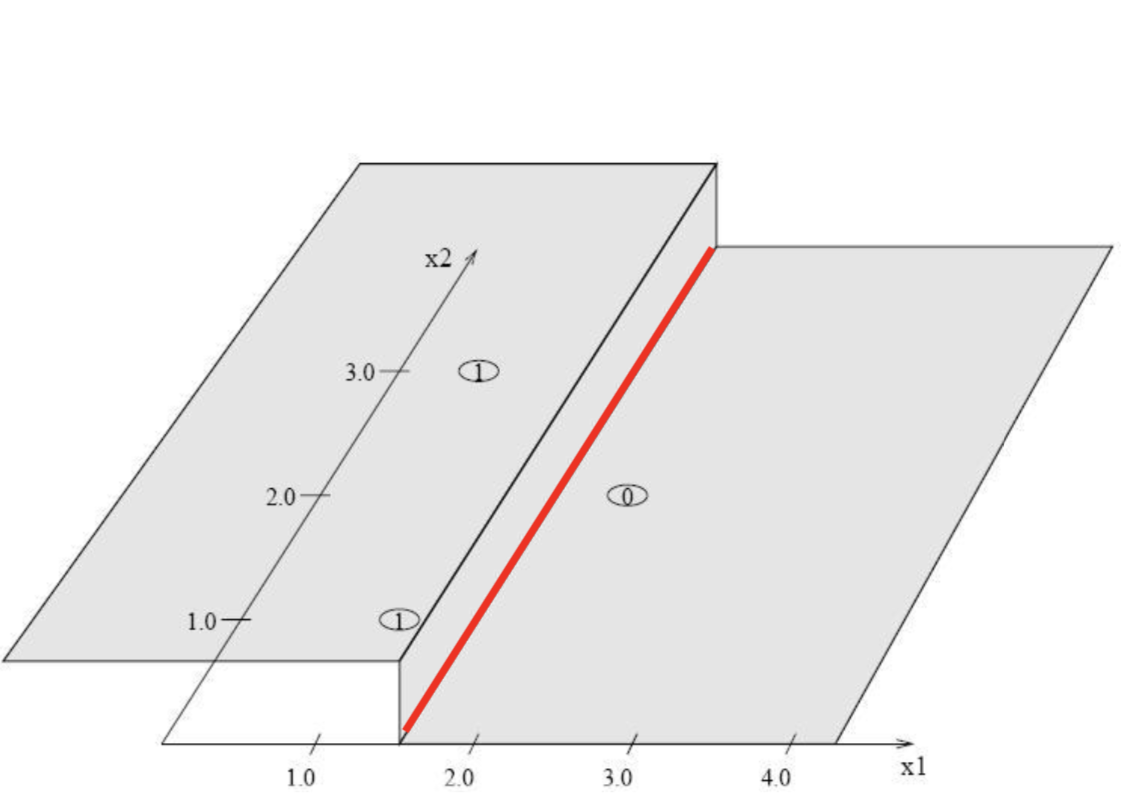
\includegraphics[scale=0.4]{Images/classificationplane.png}
\end{figure}

\subsubsection{Classificazione attraverso Decision Boundary lineare}
La classificazione può essere vista come come l'allocazione dello spazio in input in diverse regioni di decisione. Ad esempio in uno spazio di due dimensioni $x=(x_1,x_2)$ in $R^2$ e con $f(x) = 0 \lor 1$ il decision boundary sarà una retta. 
\begin{quote}
    Linear Threshold Unit (LTU) = indicatore di funzioni, quanti ne abbiamo? un insieme di divisioni indotte da iperpiani, sono tutti i modi che abbiamo per muovere la linea rossa.
\end{quote}
\begin{figure}[H]
\centering
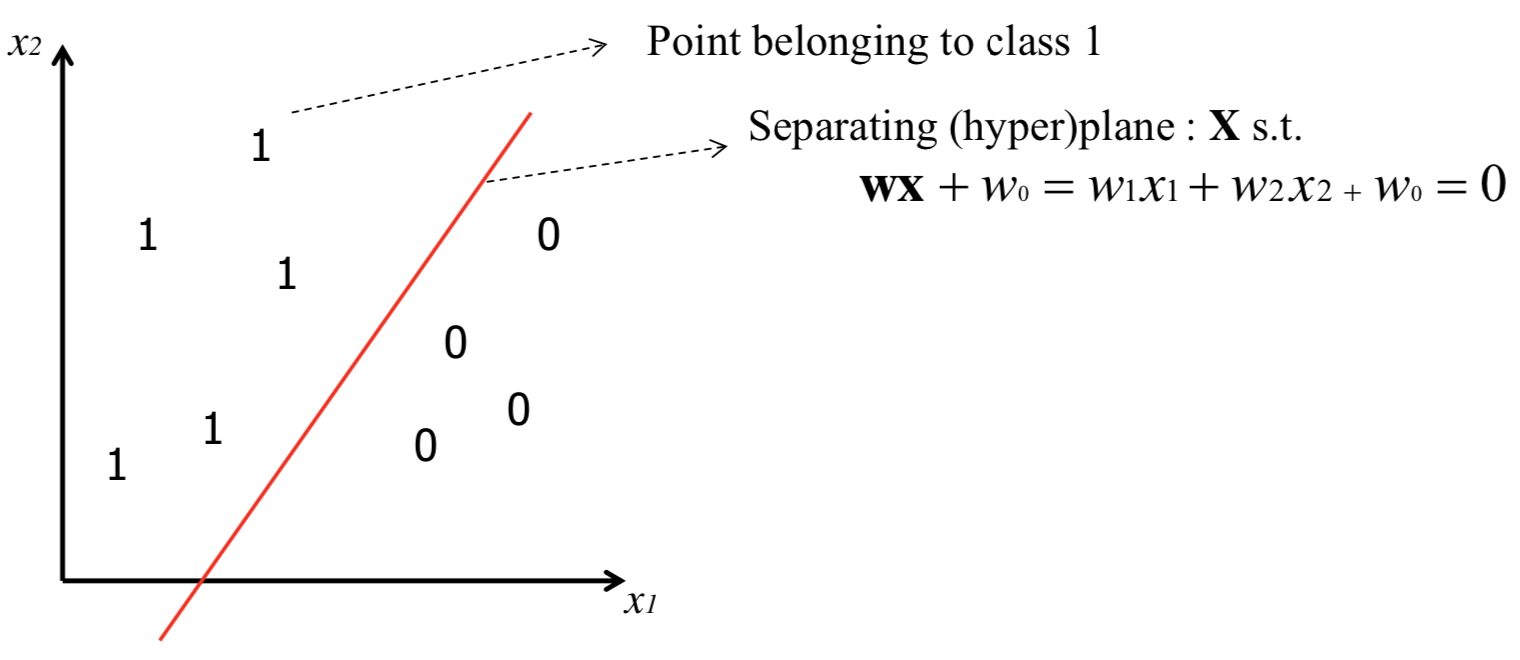
\includegraphics[scale=0.5]{Images/lineardecisionboundary.png}
\end{figure}

\subsubsection{Esempio Terremoti/Esplosioni Nucleari}
Trovare h in modo tale che il dato ($x_1, x_2$) ritorni (0 $\lor$ -1) per i terremoti e (1) per esplosioni nucleari. I dati sismici sono rappresentati da $x_1$ che é la magnitudine dell'onda del corpo e $x_2$ che é la magnitudine dell'onda della superficie. L'algoritmo trova il decision boundary.
\begin{figure}[H]
\centering
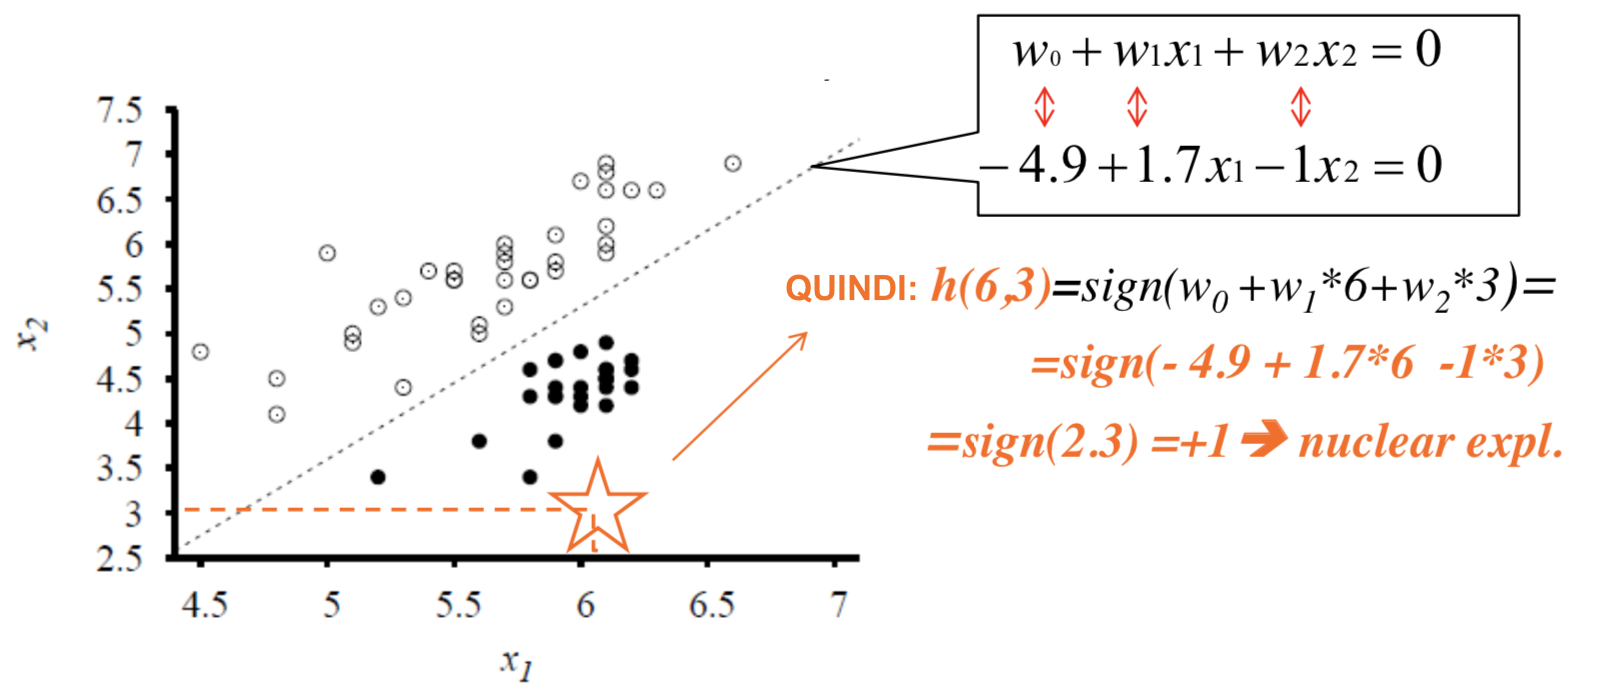
\includegraphics[scale=0.4]{Images/magnitudegraph.png}
\end{figure}

\subsubsection{Esempio Email Spam}
Trovare h(mail) in modo tale che restituisca +1 se é spam e -1 se non é una mail spam.\newline  Ad esempio $\phi(mail)$ = txtmail.contains(“denaro gratis”), w vettore di pesi per le le funzioni di input che aiutano alla previsione, cioè peso positivo per "denaro gratis", negativo altrimenti. $w^Tx$ é la combinazione dei pesi. $h_w(x)$ provvede a dare il limite per decidere se una mail é spam o non é spam.
\begin{equation}
    h_w(x)= segno(\sum_{k} w_k\phi_k(x))
\end{equation}

\subsection{Il problema di apprendimento (per classificatori lineari)}
Assumendo che usiamo ancora il metodo dei minimi quadrati, dato un insieme grande $l$ di esempi di allenamento, bisogna trovare w che minimizza la somma residua dei quadrati
\begin{equation}
    E(w)=\sum_{p = 0}^l(y_p-x_p^Tw)^2=||y-x^Tw||^2
\end{equation}
se $y_p=1$ allora $x_p^Tw \rightarrow 1$ mentre se $y_p=0\lor -1$ allora $x_p^Tw \rightarrow 0 \lor -1$. \newline 
Possiamo utilizzare l'algoritmo di discesa del gradiente:
\begin{equation}
    \Delta w_i = - \frac{\partial E(w)}{\partial w_i} = \sum_{p=1}^l (y_p - (x_p^Tw)) * x_{p,i}
\end{equation}
Nella derivata ignoriamo il 2 che viene fuori dal quadrato. È una costante che non incide sull'eta (il coefficiente di apprendimento).

\subsubsection{$\Delta w$ come regola della correzione dell'errore}
\begin{figure}[H]
\centering
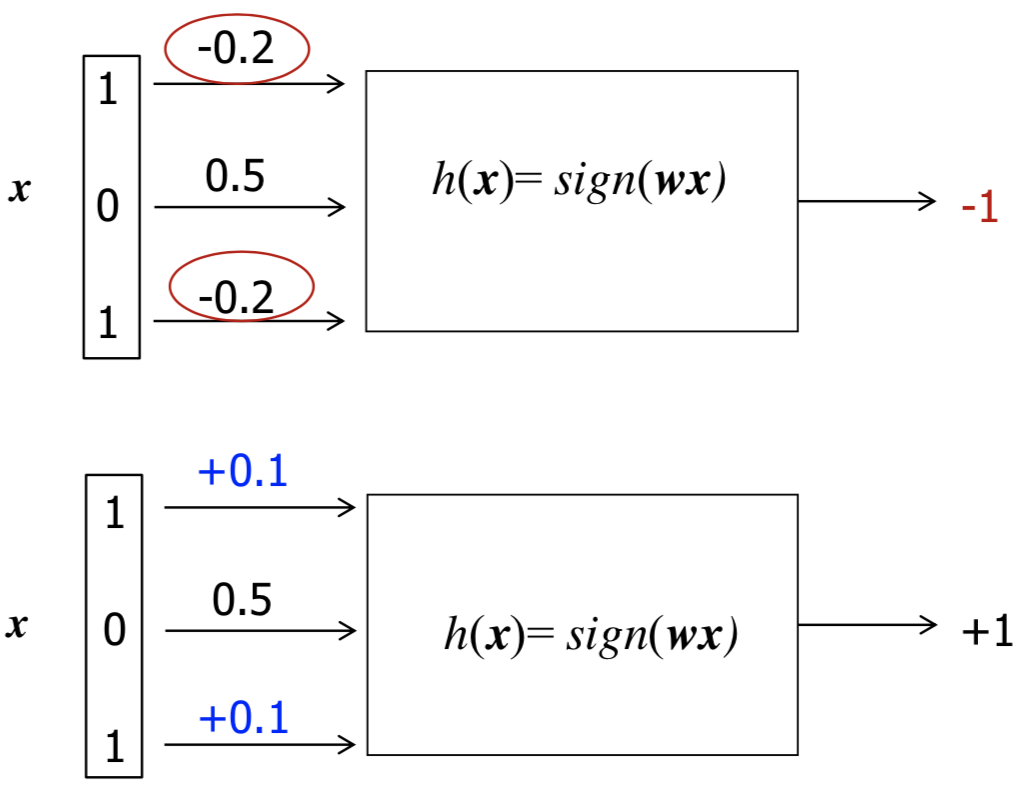
\includegraphics[scale=0.4]{Images/errorcorrection.png}
\end{figure}
Se un input viene classificato erroneamente dalla funzione $h(x)=segno(w^Tx)$, quindi ad esempio il $\Delta$ negativo per $w_1$ e $w_3$, bisogna aumentare $w_1$ e $w_3$ proporzionalmente (con il coefficiente eta). Eseguiamo una correzione d'errore alzando i valori dove sono troppo bassi, e viceversa.

\subsection{Classificazione dei pattern}
Il modello viene $allenato$ su un insieme di esempi con il calcolo LMS su $w^Tx$ dall'algoritmo di discesa del gradiente, usato per la regressione lineare. Il modello viene $utilizzato$ per la classificazione applicando la funzione di soglia $h(x)=segno(w^Tx)$. L'errore può essere calcolato come errore di classificazione o numero di pattern classificati erroneamente. 
\begin{equation}
  L(h(x_p),d_p)=\begin{cases}
    0 & \text{se $h(x_p)=d_p$}.\\
    1 & \text{altrimenti}.
  \end{cases}
  \quad mean\_err = \frac{1}{l}\sum_{i=1}^l L(h(x_i), d_i)
\end{equation}
dove $d_p$ é l'output dato dagli esempi di allenamento, quindi stiamo classificando i valori calcolati dalla nostra h con i valori degli esempi etichettati.
\begin{quote}
    Accuratezza = media dei pattern correttamente classificati = $(l-numerr)/l$ \newline dove $numerr=\sum_{i=1}^l L(h(x_i), d_i)$
\end{quote}
L'algoritmo é lo stesso come per la regressione $\rightarrow$ Algoritmo gradiente discendente (anche l'espansione lineare e Tikhonov possono essere applicati). Notare che l'algoritmo converge asintoticamente al MinLeastSquare, non necessariamente al numero minimo di errori di classificazione.

\subsection{Congiunzioni nel caso di Modello Lineare}
Possiamo rappresentare congiunzioni con i modelli lineari, ad esempio:\newline
$x_1 \land x_2 \land x_4 \Leftrightarrow y$ cioè $1x_1+1x_2+0x_3+1x_4 > 2$ dove $w_1=1, w_2=1, w_3 = 0, w_4 = 1, w_0 = 2$ (vettore dei pesi)\newline
Altro esempio con grafico: \newline
$x_1 \land x_2$ cioè $1x_1+1x_2>1$
\begin{figure}[H]
\centering
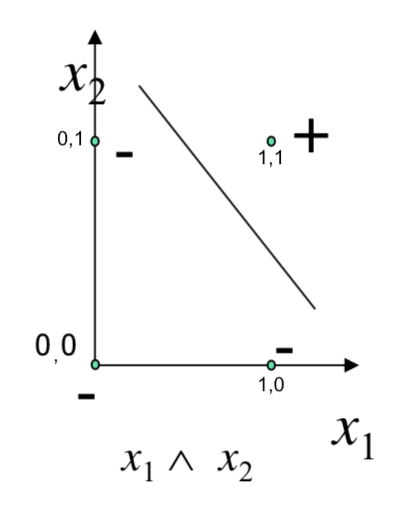
\includegraphics[scale=0.5]{Images/conjunctionsgraph.png}
\end{figure}
In generale w puó essere appreso per trovare la soluzione.

\subsubsection{Limitazioni}
Nella geometria due insiemi di punti in un grafico a due dimensioni sono linearmente separabili quando possono esser separati da una singola linea. 
\begin{figure}[H]
\centering
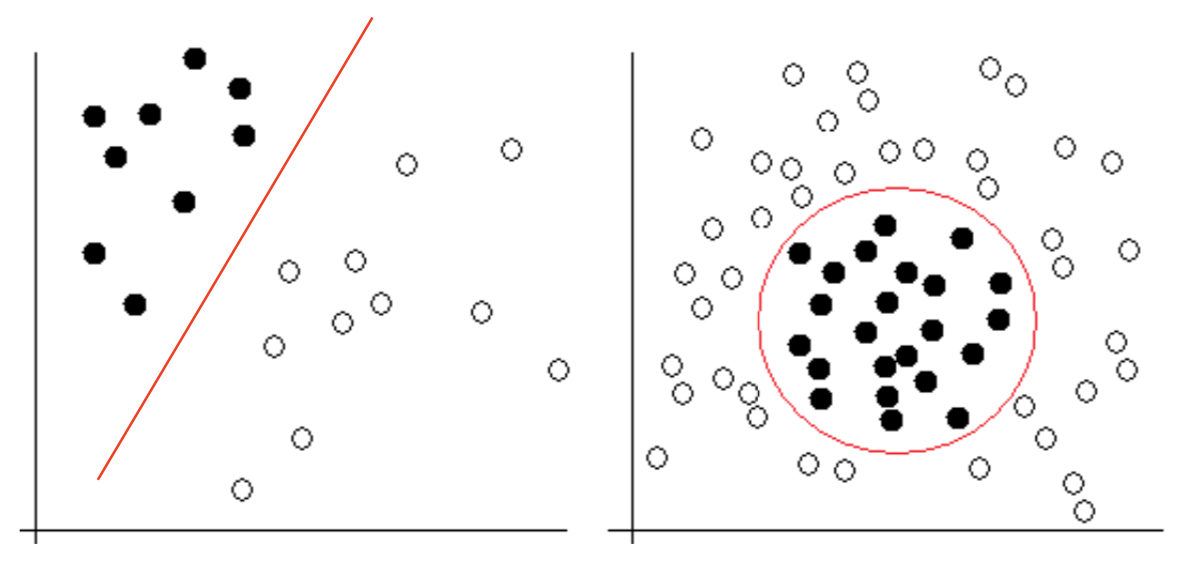
\includegraphics[scale=0.5]{Images/linearnonlinearseparation.png}
\end{figure}
In generale due gruppi di punti sono linearmente separabili in uno spazio di dimensione $n$ se possono essere separati da un iperpiano di dimensione $n-1$. Il confine lineare dà la soluzione esatta solo per insiemi di punti linearmente separabili. 

\begin{figure}[H]
\centering
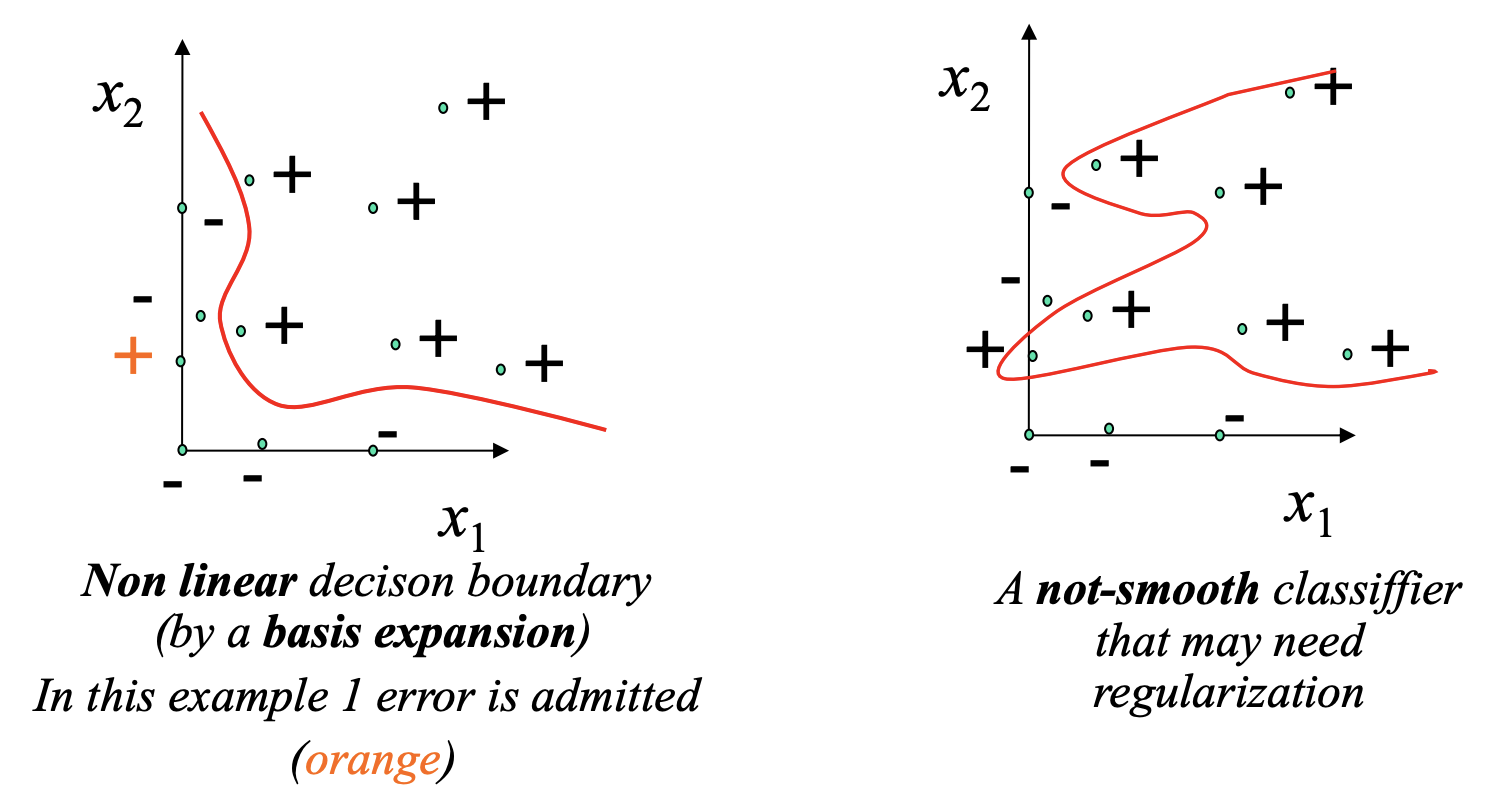
\includegraphics[scale=0.5]{Images/linearnonlinearseparation2.png}
\end{figure}

\subsection{Altri sistemi di apprendimento per la classificazione}
\begin{itemize}
    \item Linear Discriminant Analysis
    \item Logistic Regression: Stima la/le proprietà di x dato y, P(y/x) partendo modellando la densità della classe come densitá nota. Abbiamo una soglia soft (continua, differenziabile) con funzione logica (anziché soglia hard 0/1)
    \item Reti Neurali e SVM: modelli flessibili che includono approssimazione non lineare sia per la regressione che per la classificazione.
\end{itemize}

\subsection{Conclusioni sui Modelli Lineari}
I modelli lineari sono un approccio fondato di base per la regressione e la classificazione, é un modo molto compatto per rappresentare la conoscenza (tutti i dati sono nel vettore w) ma con una forte assunzione sulla relazione tra i dati (Assumiamo che ci sia una relazione lineare tra i dati, o comunque in accordo alla $\phi$ che abbiamo scelto. É una assunzione molto forte sullo spazio delle ipotesi). Abbiamo visto un algoritmo di correzione iterativa dell'errore (LMS) che ricerca spazi di ipotesi continui, una visione dei limiti ad approcci lineari e delle esigenze per modelli di ML più flessibili e anche i loro problemi: un'estensione del modello lineare per attività non lineari e un'introduzione al controllo della complessità (regolarizzazione).
\clearpage

\section{Alberi di decisione}
Un albero di decisione rappresenta una funzione che prende in input un vettore di attributi e restituisce una "decisione" (un singolo valore in output). I valori sia in input che in output possono essere valori continui, ma per adesso vedremo solo su valori discreti. Gli alberi di decisione aiutano a superare la restrizione della descrizione delle ipotesi solo tramite regole congiuntive (and). Ogni nodo dell'albero rappresenta un test su un attributo e ogni ramo corrisponde alla scelta del valore per quell'attributo, mentre le foglie corrispondono ad una classificazione. 

\subsection{Problema del PlayTennis}
Vogliamo capire in quali giorni al nostro amico piace andare a giocare a Tennis. Il nostro Training Set é il seguente:
\begin{figure}[H]
\centering
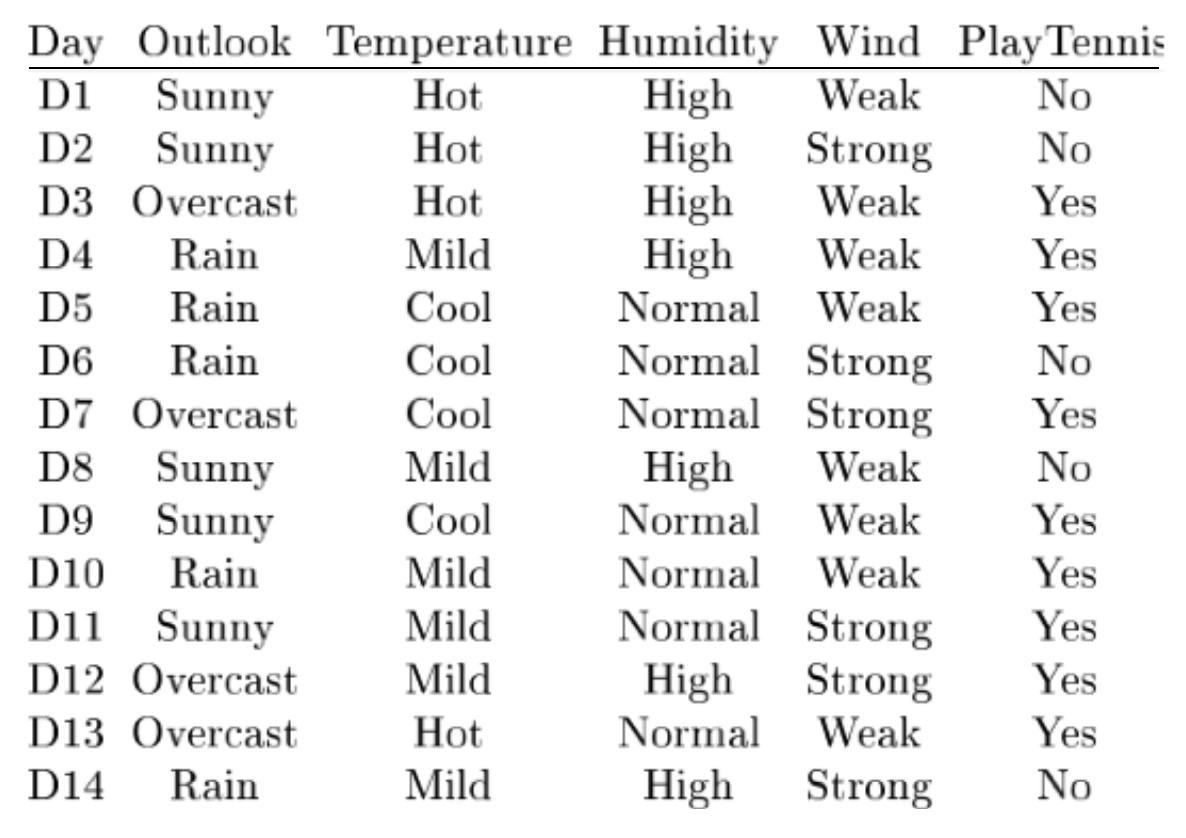
\includegraphics[scale=0.5]{Images/playtennistrainingset.png}
\end{figure}
Il nostro albero di decisione ha invece questa forma:
\begin{figure}[H]
\centering
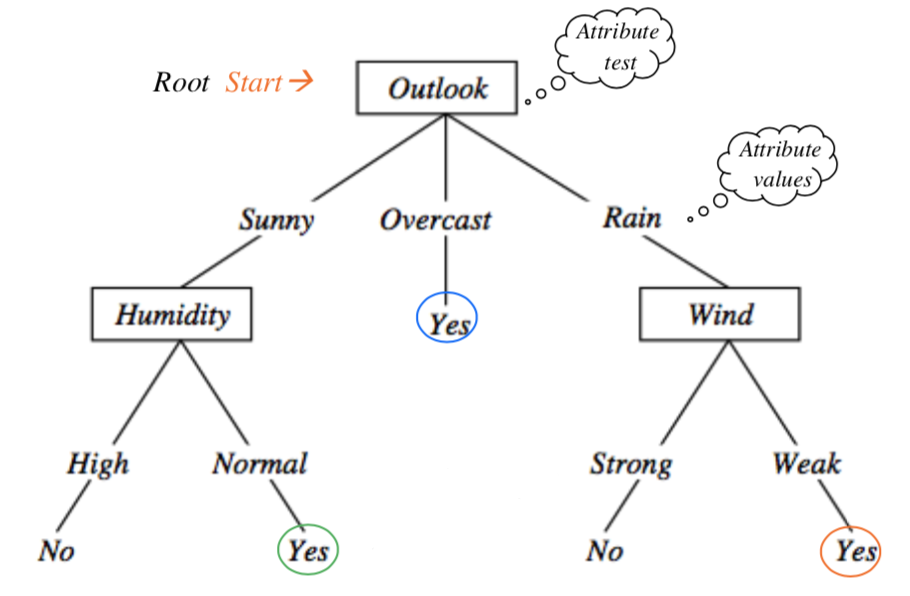
\includegraphics[scale=0.6]{Images/playtennisdecisiontree.png}
\end{figure}
\clearpage
L'albero rappresenta una disgiunzione di congiunzioni dei vincoli sui valori degli attributi, dove le foglie rappresentano la classificazione ottenuta.
In particolare il nostro albero rappresenta questa formula:
\begin{quote}
    \textcolor{green}{(Outlook=Sunny $\land$ Humidity = Normal)} $\lor$ \newline
    \textcolor{blue}{(Outlook=Overcast)} $\lor$ \newline
    \textcolor{orange}{(Outlook=Rain $\land$ Wind=Weak)}
\end{quote}
Possiamo, in altro modo, definire l'albero come un insieme di regole if-then-else.

\subsection{(Alg. ID3) Induzione Top-Down sugli alberi di decisione}
L'algoritmo ID3 é un algoritmo base per l'apprendimento che sfrutta gli alberi di decisione. Dato un insieme di esempi, l'algoritmo per la costruzione dell'albero di decisione ha un approccio Top-Down eseguendo una ricerca Greedy senza backtracking. La domanda che ci dobbiamo porre quando stiamo creando l'albero é: "qual é il prossimo attributo da testare?" che tradotto in termini di alberi di decisione é scegliere il prossimo nodo che ci restituisce più Information Gain (definito successivamente). Viene quindi creato un nodo discendente per ogni possibile valore dell'attributo e gli esempi vengono partizionati in base a quel valore. Il processo viene ripetuto per ciascun nodo successore fino a quando tutti gli esempi sono stati classificati correttamente o non sono rimasti attributi.
\begin{figure}[H]
\centering
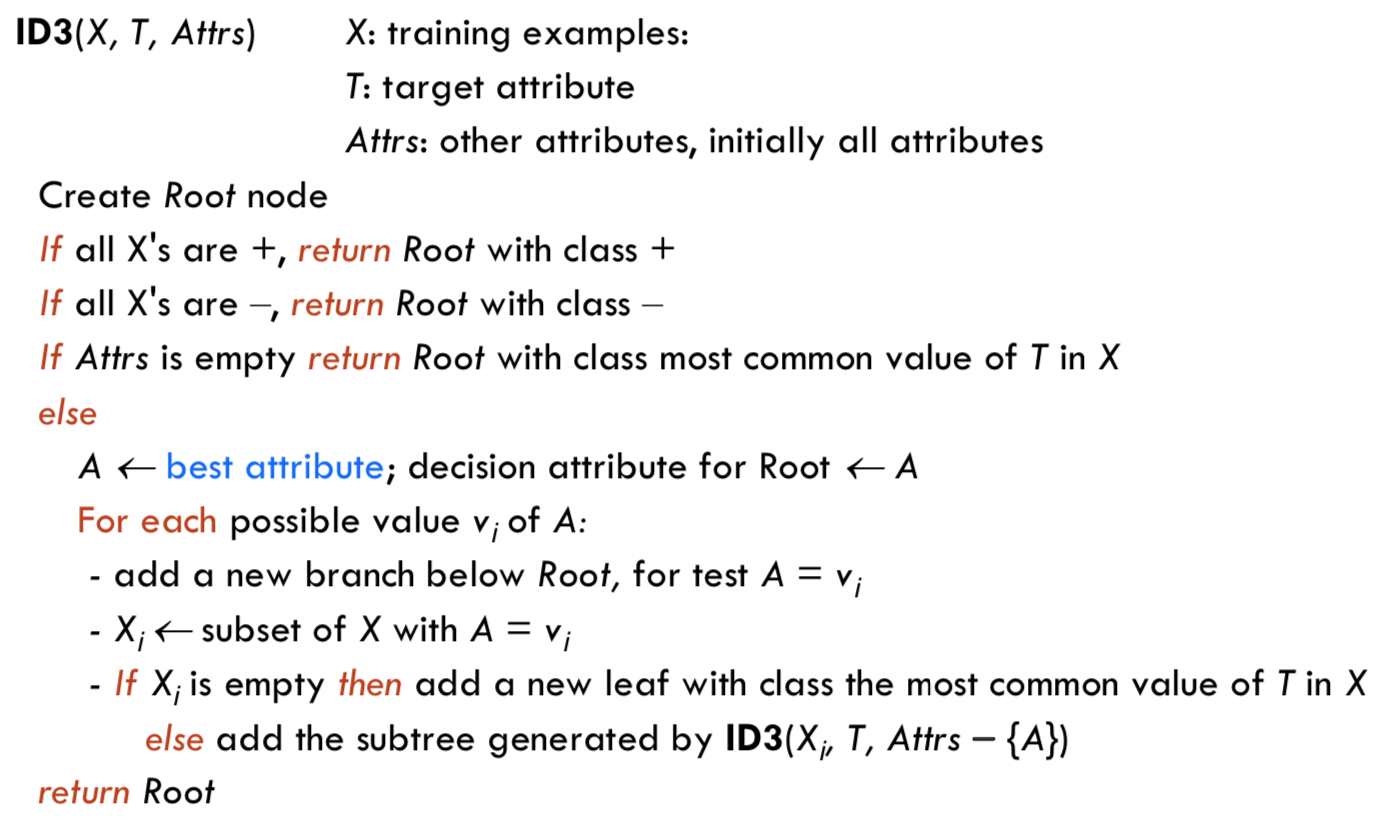
\includegraphics[scale=0.5]{Images/ID3alg.png}
\end{figure}

\subsection{Entropia: Come scegliere il miglior Attributo}
La scelta principale in ID3 riguarda quale attributo testare ad ogni nodo. Per definire l'Information Gain dobbiamo usare la nozione di entropia, la quale misura l'impurità di una collezione di esempi.
\begin{itemize}
    \item S é una collezione di esempi
    \item $p_+$ é una porzione di esempi positivi in S
    \item $p_-$ é una porzione di esempi negativi in S
\end{itemize}
\begin{quote}
    $Entropy(S)=-p_+ log_2 p_+ -p_- log_2 p_-$
\end{quote}
\begin{figure}[H]
\centering
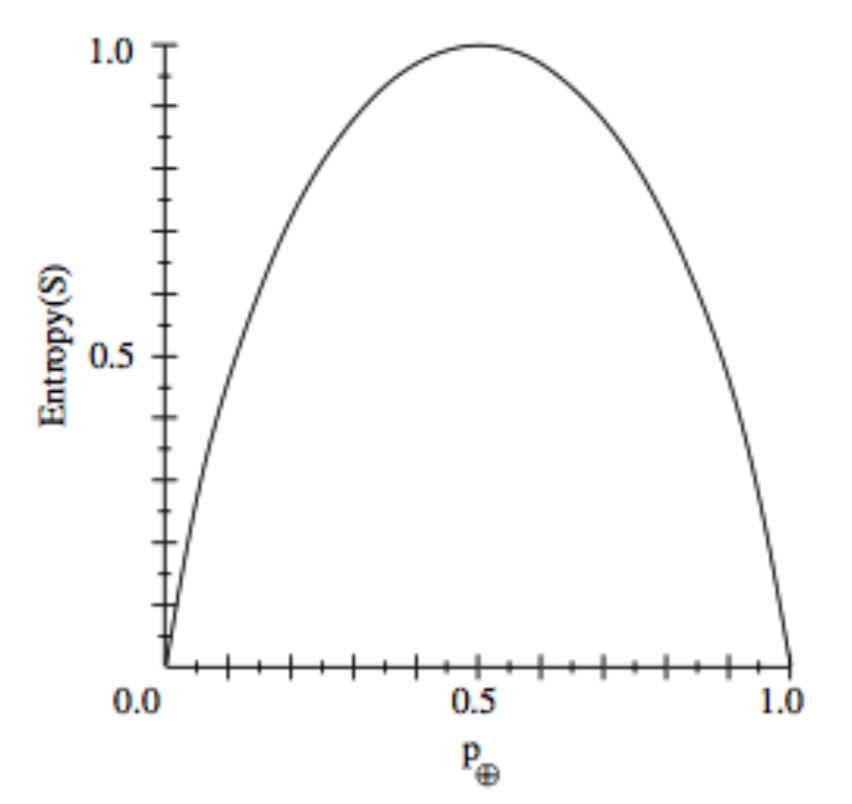
\includegraphics[scale=0.5]{Images/entropygraph.png}
\end{figure}
Se gli esempi sono tutti positivi o tutti negativi (quindi appartengono tutti alla stessa classe) otteniamo una entropia che vale 0. Otteniamo una entropia massima se gli esempi positivi e negativi sono in ugual dimensione ($\frac{1}{2}+,\frac{1}{2}-$). \newline 
Prendiamo come esempio S=14 attributi:
\[Entropy([14+,0-])=-\frac{14}{14}log_2(\frac{14}{14}) - 0 log_2 0 = 0\]
\[Entropy([7+,7-])=-\frac{7}{14}log_2(\frac{7}{14}) - \frac{7}{14}log_2(\frac{7}{14}) = 1\]
\[Entropy([9+,5-])=-\frac{9}{14}log_2(\frac{9}{14}) - \frac{5}{14}log_2(\frac{5}{14}) = 0.94\]
Sia l'entropia che la variabile p hanno valori tra lo 0 e 1 compresi. Una interpretazione dell'entropia é che essa specifica il numero minimo di bit necessari per rappresentare la classificazione si un membro random di S, per questo si utilizza il logaritmo in base 2.
\subsection{Information Gain}
L'Information Gain misura la riduzione aspettata dell'entropia causata dal partizionamento degli esempi rispetto all'attributo. Cioè: 
\begin{equation}
    Gain(S,Attr)=Entropy(S)-\sum_{v \in Values(Attr)}\frac{|S_v|}{|S|}Entropy(S_v)
\end{equation}
dove Values(Attr) é l'insieme dei possibili valori associabili all'attributo, mentre $S_v$ é il sottoinsieme degli esempi S per i quali l'attributo ha valore v. \newline 
Notare come il primo membro dell'equazione é l'entropia su tutto l'insieme S, mentre il secondo é l'entropia attesa dopo che S é stato partizionato secondo l'attributo Attr.
Maggiore è l'Information Gain, più efficace è l'attributo nella classificazione dei dati di training. Usiamo l'entropia per misurare l'omogeneità della classe del sottoinsieme degli esempi, quindi dobbiamo scegliere Attr in modo tale da massimizzare il Gain. Stiamo sottraendo $\sum_{v \in Values(Attr)}\frac{|Sv|}{|S|}Entropy(Sv)$ all'entropia generale, ci aspettiamo di ottenere una maggiore omogeneità e quindi un Information Gain maggiore. Lo scopo é quello di separare gli esempi sulla base del target, trovando l'attributo che discrimina gli esempi che appartengono a classi diverse.

\subsubsection{Esempio}
L'Information Gain viene calcolato per tutti gli attributi, e ID3 lo sfrutta (prende quello con Inf. Gain maggiore) per scegliere il prossimo attributo da testare. Nel nostro esempio Gain(S,Outlook)=0.246 ed é quello con information gain maggiore rispetto a agli altri 3. Quindi per il nodo radice é stato scelto l'attributo Outlook. I dati vengono partizionati rispetto ai valori di Outlook e associati ai nodi successivi. Notiamo che se Outlook=Overcast la risposta é sempre YES, quindi andiamo a valutare $Gain(S_{Sunny},Humidity)$, $Gain(S_{Sunny},Temperature)$ e $Gain(S_{Sunny},Wind)$. Trovando che il massimo gain si ottiene con Humidity. Se l'entropia non é zero l'albero continua a crescere fino ai nodi di classificazione.
\begin{figure}[H]
\centering
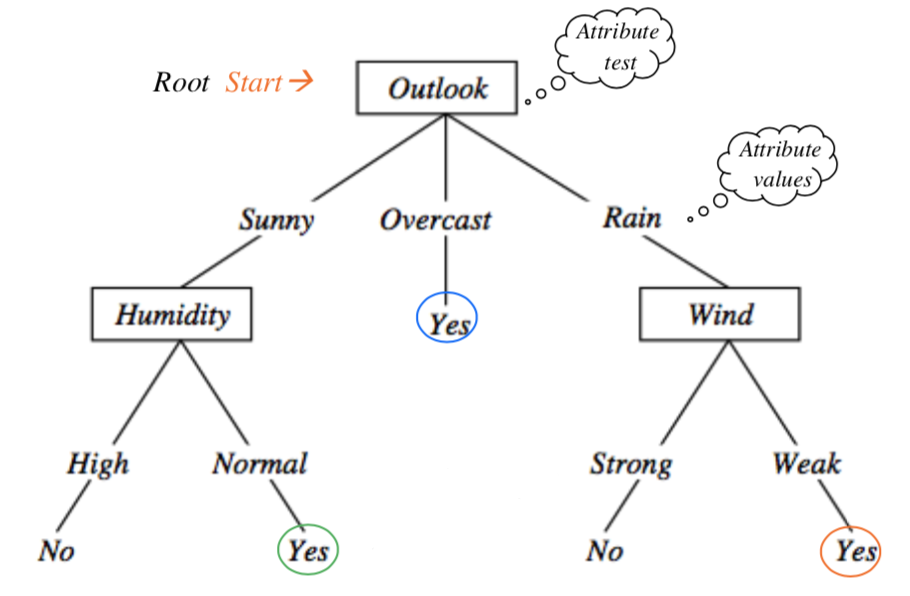
\includegraphics[scale=0.5]{Images/playtennisdecisiontree.png}
\end{figure}
\begin{figure}[H]
\centering
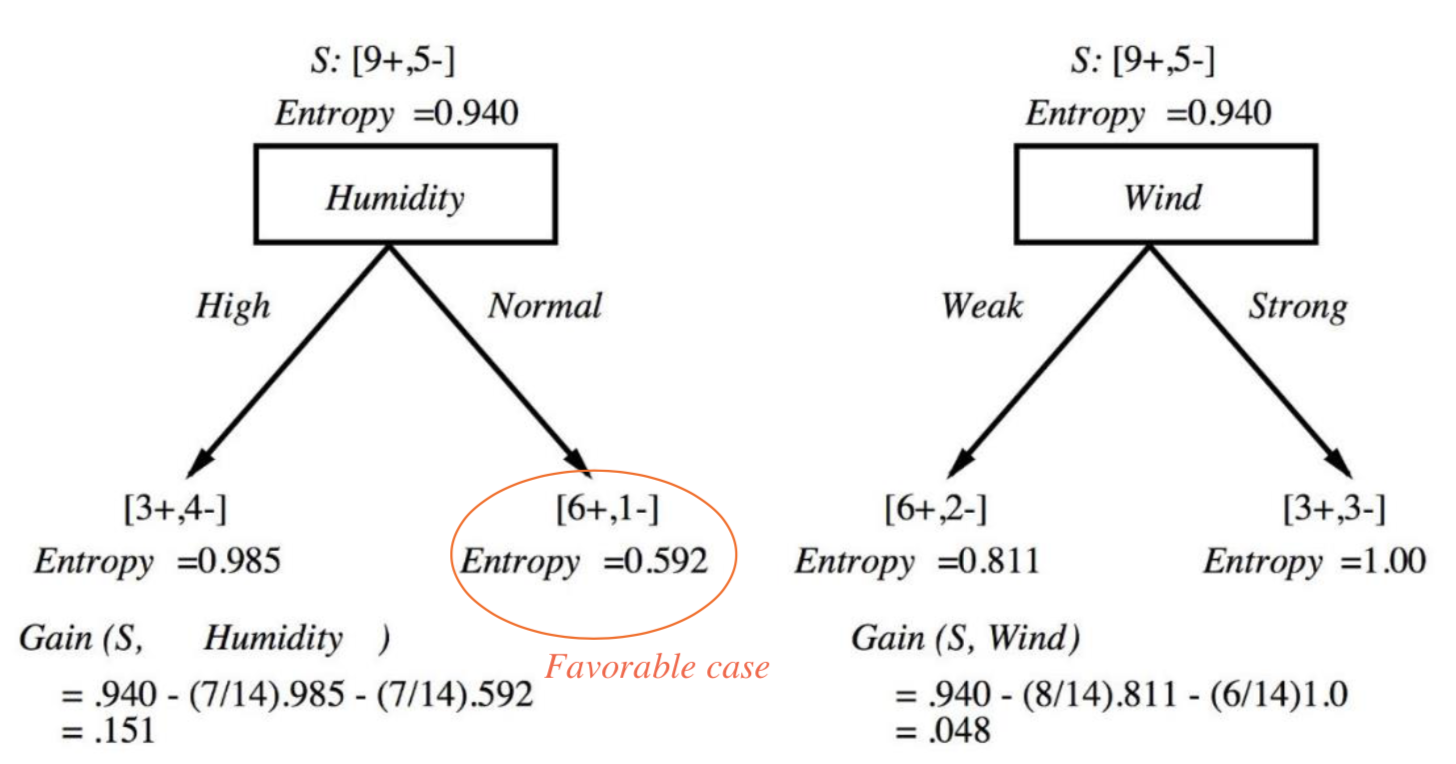
\includegraphics[scale=0.45]{Images/esempioentropia.png}
\end{figure}
Humidity fornisce piú informazioni di Wind

\subsection{Problemi con Information Gain}
L'information Gain favorisce gli attributi con molti valori possibili. Mettiamo caso che nel nostro problema PlayTennis ci fosse stato un attributo che indicava il giorno e il mese, ogni giorno a quel punto sarebbe stato un insieme puro con entropia 0 e quindi avrebbe avuto l'Information Gain più alto di tutti gli altri attributi. Facendo cosí sarebbe scelto come nodo radice, di conseguenza otterremmo un albero di profonditá 1. Ma questo mi é inutile poiché il giorno non é un valore significativo per classificare le istanze future che ancora non abbiamo visto. Quindi come evitiamo la creazione di piccoli sottoinsiemi che mi riducono la generalizzazione?

\subsection{Gain Ratio}
\begin{equation}
    GainRatio(S,Attr)=\frac{Gain(S,Attr)}{SplitInformation(S,Attr)}
\end{equation}
dove
\begin{equation}
    SplitInformation(S,Attr)=-\sum_{i=1}^c \frac{|S_i|}{|S|}log_2\frac{|S_i|}{|S|}
\end{equation}
dove c é il numero di variabili possibili per quell'attributo. $S_i$ sono gli insiemi ottenuti partizionando sul valore i di Attr. \newline 
SplitInformation misura l'entropia di S rispetto ai valori di A. Più i dati sono dispersi in modo uniforme, più è alto. GainRatio penalizza gli attributi che dividono gli esempi in tante piccole classi come per l'esempio dell'attributo della data. Sia $| S | = numerodate$ divide gli esempi in n sottogruppi.
\begin{equation}
    SplitInformation(S, Date)= -[(\frac{1}{n} log_2 \frac{1}{n})+...+ (\frac{1}{n}log_2 \frac{1}{n})]= - log_2\frac{1}{n} =log_2n
\end{equation}
Il problema che può nascere é che lo SplitInformation può essere 0 o molto piccolo quando $|S_i|$ é circa $|S|$ per alcuni valori i. Ad esempio in un caso estremo in cui $|S_1|=0$ e $|S_2|=1$ otteniamo uno $SplitInformation = -[0/n * log 0/n + n/n * log n/n] = - 0 - 0 = 0$. Per evitare questo effetto viene utilizzata la seguente euristica:
\begin{enumerate}
    \item Calcolare il Gain per ogni attributo
    \item Applicare il GainRatio solo a quegli attributi con il Gain superiore alla media
\end{enumerate}

\subsection{Considerazioni sulla ricerca nello Spazio delle Ipotesi (in DT Learning)}
Nell'algoritmo ID3 la ricerca nello spazio consiste nella ricerca dell'albero dal più semplice al più complesso. Mettendolo a confronto con l'algoritmo Candidate Elimination troviamo che:
\begin{itemize}
    \item Lo spazio delle ipotesi é completo perché rappresenta tutte le funzioni a valori discreti relative agli attributi disponibili (mentre prima avevamo solo funzioni rappresentate da and)
    \item La ricerca mantiene solo una singola ipotesi corrente perché è un albero di decisione (mentre prima si manteneva il set di tutte le ipotesi consistenti)
    \item ID3 nella sua forma pura non utilizza backtracking e non c'è garanzia di trovare l'ottimo (perché é un algoritmo greedy e potrebbe fermarsi sui minimi locali)
    \item Usa tutti gli esempi a disposizione (mentre prima si guardava un esempio alla volta, in ID3 si usa tutto l'insieme degli esempi, siamo meno suscettibili all'errore sul singolo).
    \item Può terminare prima accettando classi rumorose (mentre prima non accettavamo classi rumorose)
\end{itemize}

\subsection{Inductive Bias in DT Learning}
Qual é il nostro Inductive Bias negli alberi di decisione? Cioè qual é il modo che ha ID3 per generalizzare dagli esempi di training? \newline
L'algoritmo ID3 seleziona preferibilmente alberi corti rispetto a quelli con molti livelli e quelli che hanno un Information Gain alto vicino alla radice. Gli alberi di decisione non sono limitati nel rappresentare tutte le possibili funzioni, la restrizione non riguarda lo spazio delle ipotesi ma riguarda la strategia di ricerca. \newline
Abbiamo due tipi di Bias:
\begin{enumerate}
    \item Bias di ricerca: é legato alla strategia di ricerca. ID3 ricerca uno spazio completo di ipotesi; la strategia di ricerca è incompleta poiché essendo un algoritmo Greedy una volta che scelgo il primo attributo sto eliminando tutte le ipotesi successive che non corrispondono.
    \item Bias di linguaggio: é legato all'insieme delle ipotesi esprimibili o considerabili. Candidate Elimination cerca uno spazio di ipotesi incompleto ma la strategia di ricerca è completa.
\end{enumerate}
Perché preferiamo un Bias di ricerca? Se iniziamo con uno spazio di ricerca troppo stringente potremmo escludere la funzione target. Conviene avere uno spazio più ampio che poi andiamo a restringere con la strategia di ricerca \footnote{Rasoio di Occam: "prefer the simplest hypothesis that fits the data"}. In ML generalmente si usano approcci flessibili (capacità universale dei modelli), senza escludere a priori la funzione target sconosciuta ma ovviamente, flessibile $\rightarrow$ Overfitting!

\subsection{Problemi con gli alberi di decisione}
Il problema principale che può presentarsi quando si usano gli alberi di decisione é l'Overfitting (errore di taglio ridotto). Costruire alberi che si adattano troppo agli esempi di training portano all'Overfitting. Definiamo l'errore di una ipotesi h su:
\begin{itemize}
    \item Dati di training: $error_D(h)$ //errore empirico
    \item Tutti i dati contenuti in X: $error_X(h)$ //errore atteso
\end{itemize}
\begin{quote}
    L'ipotesi h "overfitta" i dati di allenamento se c'é un'altra ipotesi h' tale che: \newline
    $error_D(h)<error_D(h')$ e $error_X(h') < error_X(h)$
\end{quote}
detto a parole l'ipotesi h si comporta meglio sul singolo dato ma peggio sull'insieme di dati. Questo comporta che h' funziona male sul training set, ma molto meglio sui dati futuri non visti precedentemente. \newline
Un esempio con un dato rumoroso é il seguente: $\{Outlook=Sunny, Temp=Hot, Humidity=Normal, Wind=Strong, PlayTennis=No\}$ da come valore target NO, invece rispetto al nostro albero di decisione la risposta dovrebbe essere YES. 
\begin{figure}[H]
\centering
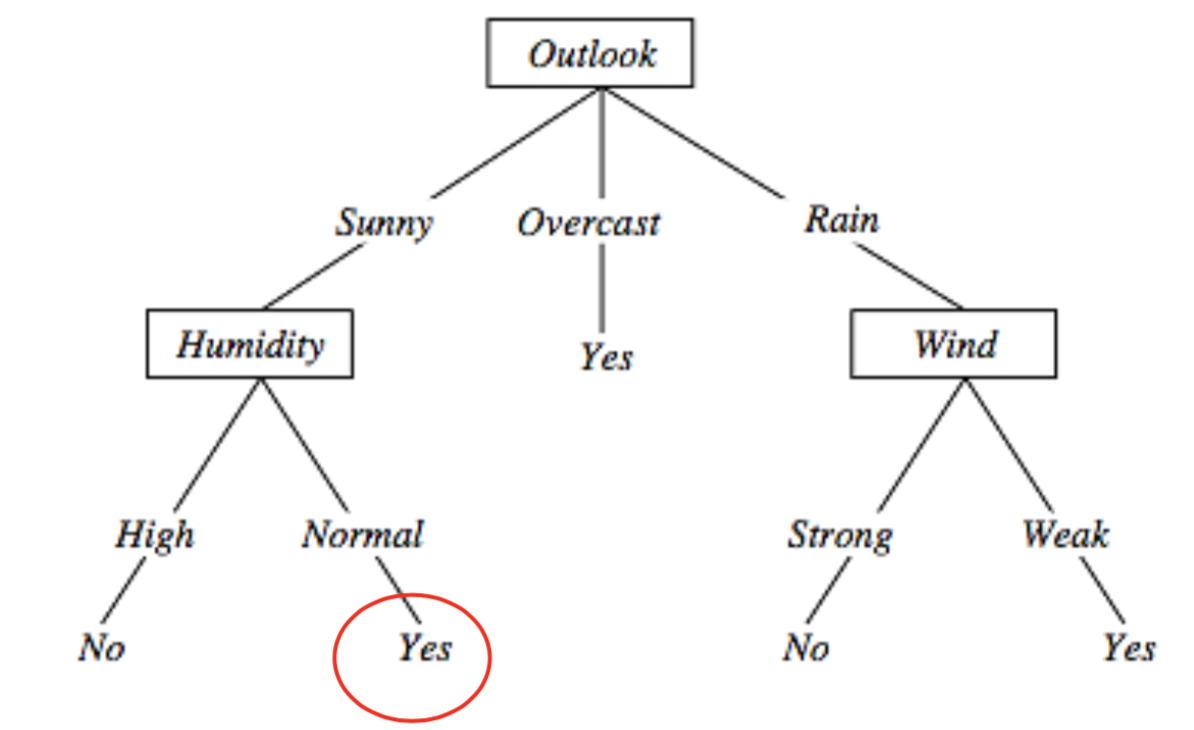
\includegraphics[scale=0.5]{Images/noisydataexampl.png}
\end{figure}
Questo nuovo esempio rumoroso provoca la divisione del secondo nodo foglia creando un albero piú complesso. Adattandosi anche al rumore, il nuovo DT è perfetto per i dati di training ma non per i nuovi dati.

\subsubsection{Evitare l'Overfitting}
Ci sono diversi approcci per evitare l'overfitting che possono essere racchiusi in due classi:
\begin{enumerate}
    \item fermare la crescita dell'albero prima che abbia una classificazione perfetta
    \item seconda é permettere all'albero di overfittare i dati e successivamente eseguire un post-potatura dei rami
\end{enumerate}
Come possiamo valutare l'effetto di queste decisioni?
\begin{itemize}
    \item Possiamo dividere il training set in due parti (training e validazione) e utilizzare il set di validazione per valutare l'utilità della post potatura
    \item Possiamo utilizzare tutti i dati di training e in seguito eseguire un test statistico per stimare l'effetto di espansione o potatura
    \item Possiamo usare un meccanismo di misurazione della complessità per la codifica degli esempi di allenamento e dell'albero. Cioè usare il principio della lunghezza minima della descrizione e fermare la crescita dell'albero quando la dimensione dell'encoding é minima.
\end{itemize}

\subsubsection{Potatura con errore ridotto}
Come possiamo usare il validation set per evitare l'overfitting? Nel reduced error pruning ogni nodo é un candidato per la potatura: la potatura consiste nella rimozione di un sottoalbero radicata in un nodo, quest'ultimo diventa una foglia e viene assegnata la classificazione più comune. I nodi vengono rimossi solo se l'albero risultante non ha prestazioni peggiori sul set di validazione. I nodi vengono eliminati in modo iterativo: ad ogni iterazione viene eliminato il nodo la cui rimozione aumenta la precisione del set di validazione. La potatura si interrompe quando nessuna potatura aumenta la precisione. Uno svantaggio é sacrificare dei dati del training set per formare il validation set.

\subsubsection{Regola della post-potatura}
Nella pratica un metodo che funziona spesso é la post-pruning rule.
Le seguenti regole sono solo euristiche: non garantiscono l'ottimo a priori.
\begin{enumerate}
    \item Si crea l'albero di decisione a partire dal training set fino a che i dati di training fittano al loro meglio. (stiamo facendo overfitting appositamente)
    \item Si converte l'albero in un insieme equivalente di regole
        \begin{itemize}
            \item Ogni path corrisponde a una regola
            \item Ogni nodo lungo un path corrisponde a una pre-condizione
            \item Ogni nodo foglia classifica
        \end{itemize}
        per esempio $(Outlook=Sunny)\land(Humidity=High) \rightarrow (PlayTennis=No)$
    \item Potare (generalizzare) ogni regola rimuovendo quelle pre-condizioni la cui rimozione migliora l'accuratezza sia sul validation set, sia sul training set.
    \item Ordinare le regole in ordine di precisione stimato e considerarle in sequenza quando si classificano nuove istanze
\end{enumerate}
Perché trasformare ogni path in regola? Ogni percorso distinto produce una regola diversa, la rimozione di una condizione può essere basata su un criterio locale. La potatura delle pre-condizioni è specifica delle regole mentre la potatura dei nodi è globale e influisce su tutte le regole!

\subsection{Problema: Valori continui degli attributi}
Fino ad ora abbiamo usato valori discreti per gli attributi, come possiamo affrontare quelli a valori continui? 
\begin{quote}
    Dato un attributo a valore continuo A, si crea dinamicamente un nuovo attributo $A_c$ tale che: $A_c = True$ se $A<c$, False altrimenti.
\end{quote} 
Ma come determinare il valore di soglia c? Un esempio sul tennis potrebbe essere: 
\begin{figure}[H]
\centering
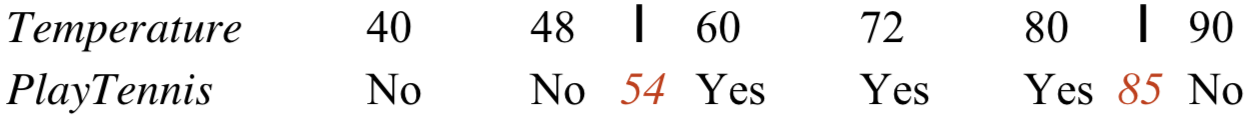
\includegraphics[scale=0.5]{Images/tempthreshold.png}
\end{figure}
Cioè possiamo determinare il valore utilizzando la media tra due esempi consecutivi dove però abbiamo un cambio di classificazione: nell'esempio (48+60)/2=54 e (80+90)/2=85.

\subsection{Problema: Dati di training incompleti}
Come possiamo invece risolvere il problema dei dati mancanti? La strategia é utilizzare altri esempi per "indovinare" l'attributo in due modi:
\begin{itemize}
    \item Si assegna il valore più comune tra tutti gli esempi di training sul nodo o quelli della stessa classe.
    \item Si assegna una probabilità a ciascun valore possibile da assegnare, in base alle frequenze, si associa il valore all'attributo mancante secondo la distribuzione di probabilità.
\end{itemize}
I valori mancanti in nuove istanze da classificare vengono trattati di conseguenza e viene scelta la classificazione più probabile.

\subsection{Problema: attributi con costi differenti}
In alcuni problemi le istanze degli attributi possono avere un costo associato, cioé possiamo dare piú importanza ad alcuni attributi rispetto ad altri. Preferiamo gli alberi che usano costi bassi per gli attributi. L'algoritmo ID3 può essere modificato per lavorare anche con i costi:
\begin{itemize}
    \item Tan e Schlimmer 
        \begin{equation}
            \frac{Gain^2(S,Attr)}{Cost(S,Attr)}
        \end{equation}
    \item Nunez
        \begin{equation}
            \frac{2^{Gain(S,Attr)}-1}{(Cost(Attr)+1)^w} \text{ con w=0/1}
        \end{equation}
\end{itemize}
\clearpage

\subsection{Visione Geometrica}
I decision boundaries, che possono essere prodotti da un albero di decisione, dividono lo spazio di input in rettangoli paralleli agli assi ed etichettano ogni rettangolo con una delle classi K (foglia dell'albero).

\begin{figure}[H]
\centering
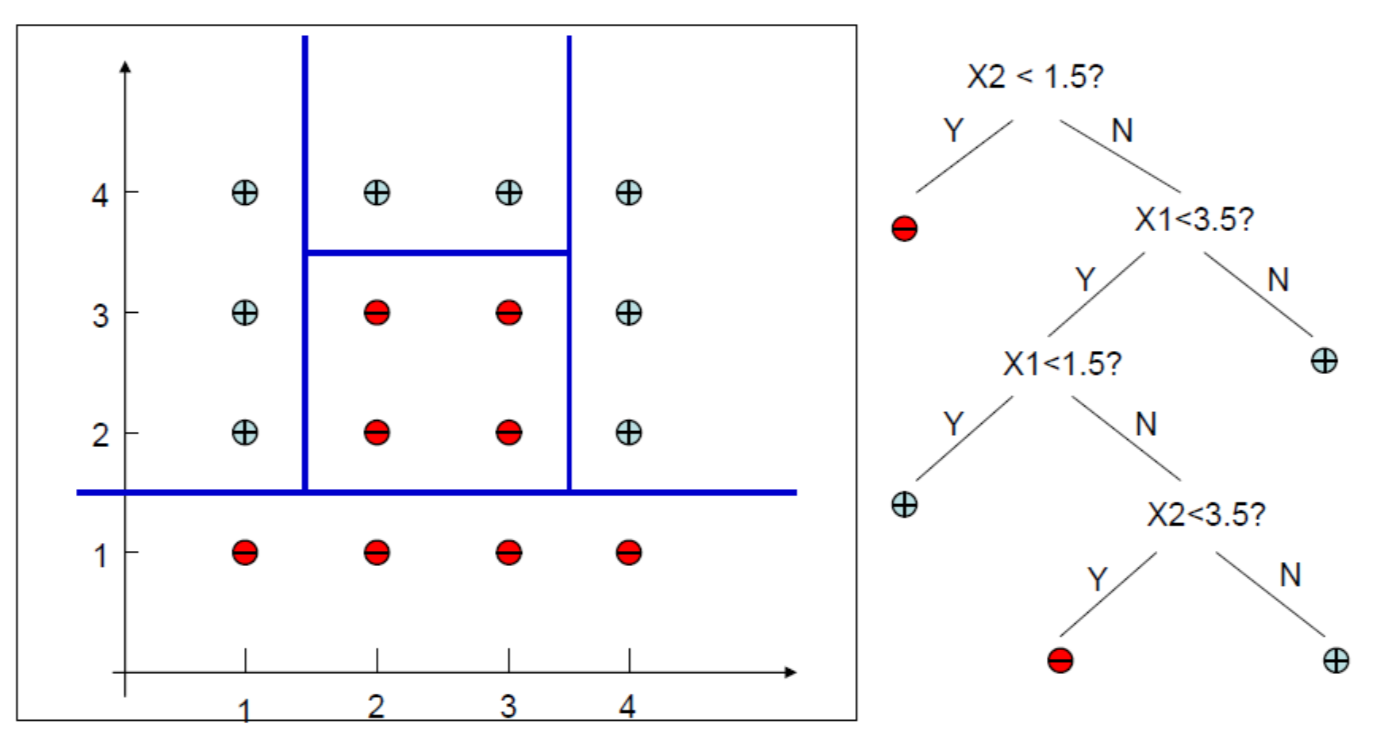
\includegraphics[scale=0.5]{Images/DTdecisionboundary.png}
\end{figure}

\subsection{Conclusioni sugli alberi di decisione}
Gli alberi di decisione sono un approccio molto utilizzato per la classificazione con un numero discreto di classi. Lo spazio delle ipotesi comprende l'area degli approcci proposizionali quindi basati su regole. Si comporta bene con dati rumorosi e gestisce anche i valori degli attributi mancanti. É facile da capire (regole if-then-else, a meno che non lo siano troppe). ID3 ricerca in uno spazio completo di ipotesi, con una strategia greedy INcompleta (perché manca il backtracking, una volta che fissa il primo nodo, non torna indietro). Presenta un approccio flessibile: l'overfitting é un problema importante che affrontata con il post-potatura e la generalizzazione delle regole indotte dall'albero.

\section{Validation}
Un problema fondamentale del ML é valutare la capacità di generalizzazione del nostro modello, una domanda che dobbiamo porci é: quando un modello é un buon modello? L'apprendimento, come abbiamo visto, consiste nel trovare una buona funzione in uno spazio di funzioni costruito a partire dai dati conosciuti. "Buona" in relazione al fatto di effettuare un basso errore di generalizzazione, per sapere quanto accuratamente il modello si comporta su nuovi dati non visti precedentemente. \newline 
In particolare, qualsiasi h (ipotesi) che approssima bene f (la nostra funzione da cercare) sui dati di training, approssimerà bene anche su istanze non conosciute? La generalizzazione é quindi un punto cruciale del ML, dobbiamo trovare un modo in cui scegliamo il miglior modello tra svariati modelli calcolati.
Abbiamo visto che si procede con una fase di apprendimento (Learning phase) dove si costruisce (training, fitting) il modello sfruttando i dati conosciuti. Segue poi una fase predittiva (Predictive phase) dove si applica il modello a nuovi dati sconosciuti e si valuta l'ipotesi predittiva (ad esempio si valuta la capacità di generalizzazione), quest'ultima é una fase di test. \newline
Per effettuare questa valutazione usiamo due misurazioni:
\begin{itemize}
    \item Per la classificazione: Mean Square Error sulla funzione di Loss e l'accuratezza o Mean Error Rate per il risultato.
    \item Per la regressione: Mean Square Error, Mean Absolute Error ma anche valori statistici come R chiamato coefficiente di correlazione
\end{itemize}

\subsection{Obiettivi Validazione}
La validazione ha due obiettivi principali:
\begin{itemize}
    \item Model Selection: stima la performance (errore di generalizzazione) di differenti modelli di apprendimento in modo tale da scegliere il migliore. Il compito di selezione del modello ovviamente restituisce un modello.
    \item Model Assessment: dopo aver scelto un modello finale, stimiamo/valutiamo il suo errore/rischio di previsione (errore di generalizzazione) su nuovi dati di test mai visti prima (magari dati dal cliente). Il compito di valutazione di un modello restituisce una stima.
\end{itemize}

\subsection{Holdout Cross-Validation}
Per ottenere una valutazione accurata di un modello dobbiamo valutarlo su esempi nuovi mai visti. Ma noi abbiamo solo un insieme dati limitati e non dobbiamo sprecarli. Dobbiamo quindi suddividere il nostro data set D in Training Set, Validation Set e Test Set.
\begin{figure}[H]
\centering
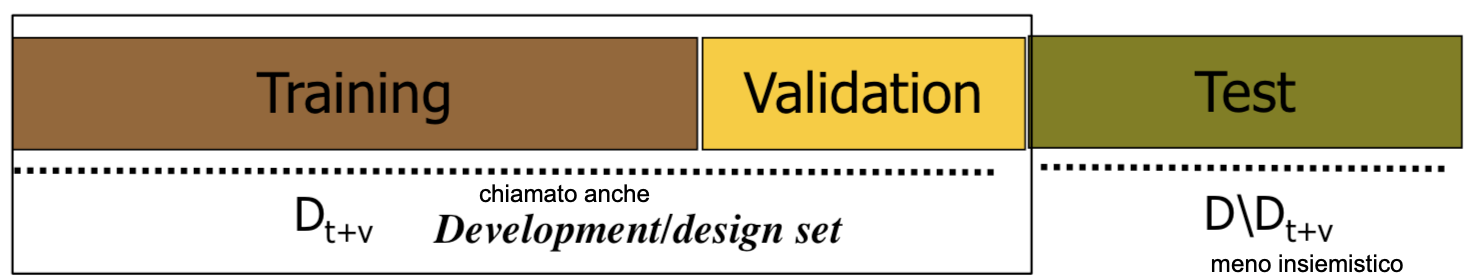
\includegraphics[scale=0.5]{Images/modelselectiontrvts.png}
\end{figure}
Il Training Set verrà usato dall'algoritmo per la creazione dell'ipotesi h. Il Validation Set viene usato per scegliere il miglior modello tra differenti modelli costruiti. Infine usiamo il Test Set solo per la valutazione del modello.\newline
Cosa succede se il test set viene utilizzato in un ciclo ripetuto di design? Stiamo eseguendo una selezione del modello e non una valutazione dell'errore di generalizzazione affidabile. Purtroppo non saremo in grado di valutare il modello su esempi non visti, poiché ormai "ce li siamo bruciati". In questo caso, dato che abbiamo usato il test set abbiamo una valutazione sovraottimistica. La regola d'oro é tenere una separazione tra i compiti e usare insiemi separati per Training, Validation e Test.

\subsection{Meta-Algoritmo per l'utilizzo del Data Set}
\begin{itemize}
    \item separare TR, VL e TS
    \item cercare la migliore ipotesi $h_{w,\lambda}$ cambiando gli iper-parametri $\lambda$ del modello
    \item per ogni valore differente dell'iper-parametro $\lambda$: cercare la migliore ipotesi che minimizza l'errore / perdita empirica (fittando i dati sul TR set) trovando i migliori parametri w.
    \item selezionare la migliore ipotesi $h_{w,\lambda}$ dove migliore significa con il minor errore sul Validation Set!
    \item opzionale: é possibile far fittare h su TR+VL con $\lambda$ ormai fissato
    \item valutare la h finale sul Test Set
\end{itemize}
\clearpage

La ricerca dei migliori iper-parametri può consistere in una ricerca in una griglia di valori candidati, per ogni modello calcolare il risultato su Validation Set e prendere quello che con il minimo errore a massima accuratezza. 
\begin{figure}[H]
\centering
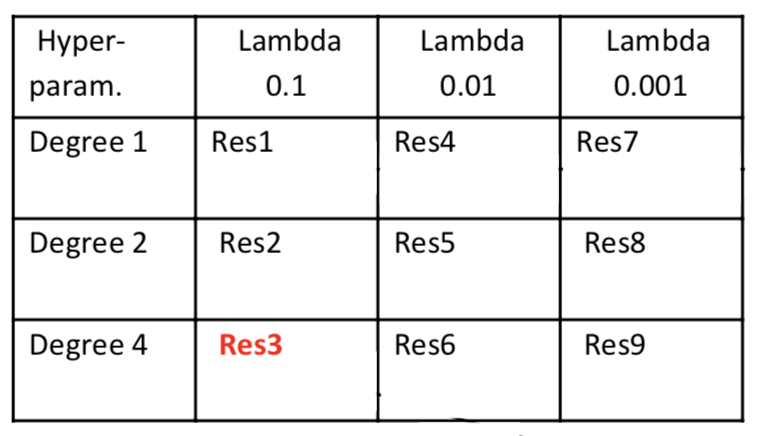
\includegraphics[scale=0.5]{Images/hypergrid.png}
\end{figure}
Nell'immagine Res1 é calcolato sul Validation Set dal modello con un polinomio di grado 1 e un $\lambda$ = 0.1 (modello allenato sul training set). Il migliore é Res3, perché ha un polinomio di grado 4 e $\lambda$ = 0.1. Questi calcoli sono facili da parallelizzare.

\subsubsection{Esempio}
\begin{figure}[H]
\centering
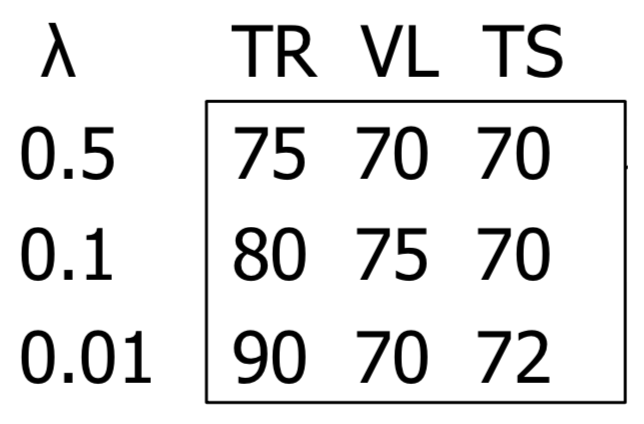
\includegraphics[scale=0.5]{Images/trvltsexample.png}
\end{figure}
\begin{itemize}
    \item In che ordine si usano le porzioni di dati per calcolare i valori in tabella? \newline
    Prima il training, poi validation e infine il test
    \item Quale modello (ossia lambda) si sceglie? \newline 
    Si sceglie il migliore sul Validation Set, NON si usa il Test Set per il model selection!
\end{itemize}

\subsubsection{Esempio perché separare VL e TS}
Ci troviamo in una situazione con 20-30 esempi, 1000 variabili di input, come output abbiamo target 0/1 calcolato randomicamente. Trovo un modello con una sola variabile che indovina "per caso" al 99\% su training e validation set. Otteniamo un risultato perfetto (cioé un modello con accuratezza al 99\%)? 99\% non é una buona stima dell'errore di test (quella corretta é 50\% visto che gli 0/1 in output sono randomici). L'errore stimato su training o validation per il model selection NON é utile! Usare tutto il data set per feature/model selection lede la correttezza della stima. Se effettuo la selezione del modello su tutto il data set e poi eseguo training e validation su sottoinsiemi, il test fornirà risultati biased (FS-bias). Un test set esterno fornisce invece la stima corretta del 50\%.

\subsection{K-fold cross validation}
\begin{figure}[H]
\centering
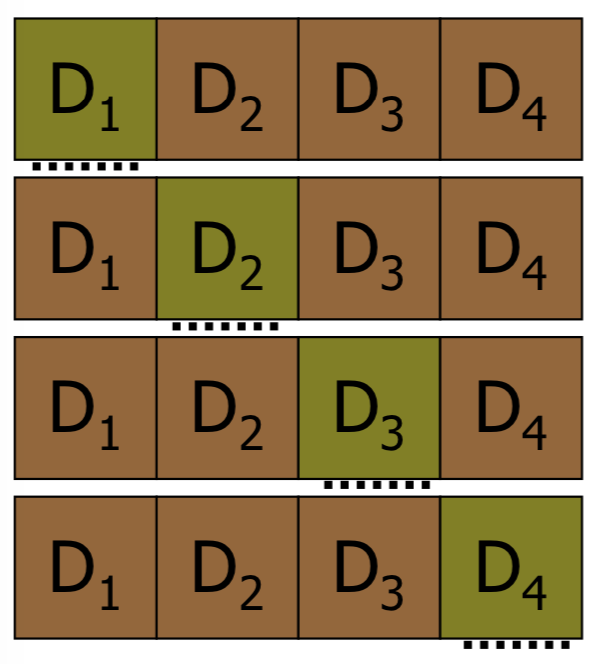
\includegraphics[scale=0.5]{Images/kfold.png}
\end{figure}
Hold out cross validation, che abbiamo visto prima, può effettuare un uso insufficiente di dati. Il seguente metodo ogni volta riparte da zero e non tiene conto di quello che é successo prima. \newline
K-fold cross validation:
\begin{quote}
    Scegliere un $\lambda$. Dividere il data set in $D$ porzioni mutualmente esclusive di dati. Allenare l'algoritmo di apprendimento sull'insieme $D - D_i$ e testarlo su $D_i$. Calcolo la media sui risultati trovati su $D_i$. Cambio $\lambda$ e rieseguo il tutto. Alla fine scelgo il modello con il minimo errore di validation, sulla base del valore calcolato con la media sui vari $D_i$.
\end{quote}
Utilizza tutti i dati per training, validazione o test. NOTA: questa tecnica può essere utilizzata sia per il validation set, sia per il test set. In quante parti dobbiamo dividere? 3,5,10... ma spesso é computazionalmente costoso. 

\subsection{Esempio di Model Selection e Assessment}
Dividere i dati in Training Set e Test Set (sfruttando Hold out o K-fold), usare K-fold internamente sul Training Set per trovare i migliori iper-parametri $\lambda$ del modello. Eseguire una ricerca su griglia con tutti i possibili valori dell'iper-parametro e scegliere il miglior $\lambda$. A questo punto allenare su tutto il TR set il modello finale e valutarlo su un test set esterno.

\subsection{Comportamento tipico di un algoritmo di apprendimento}
\begin{figure}[H]
\centering
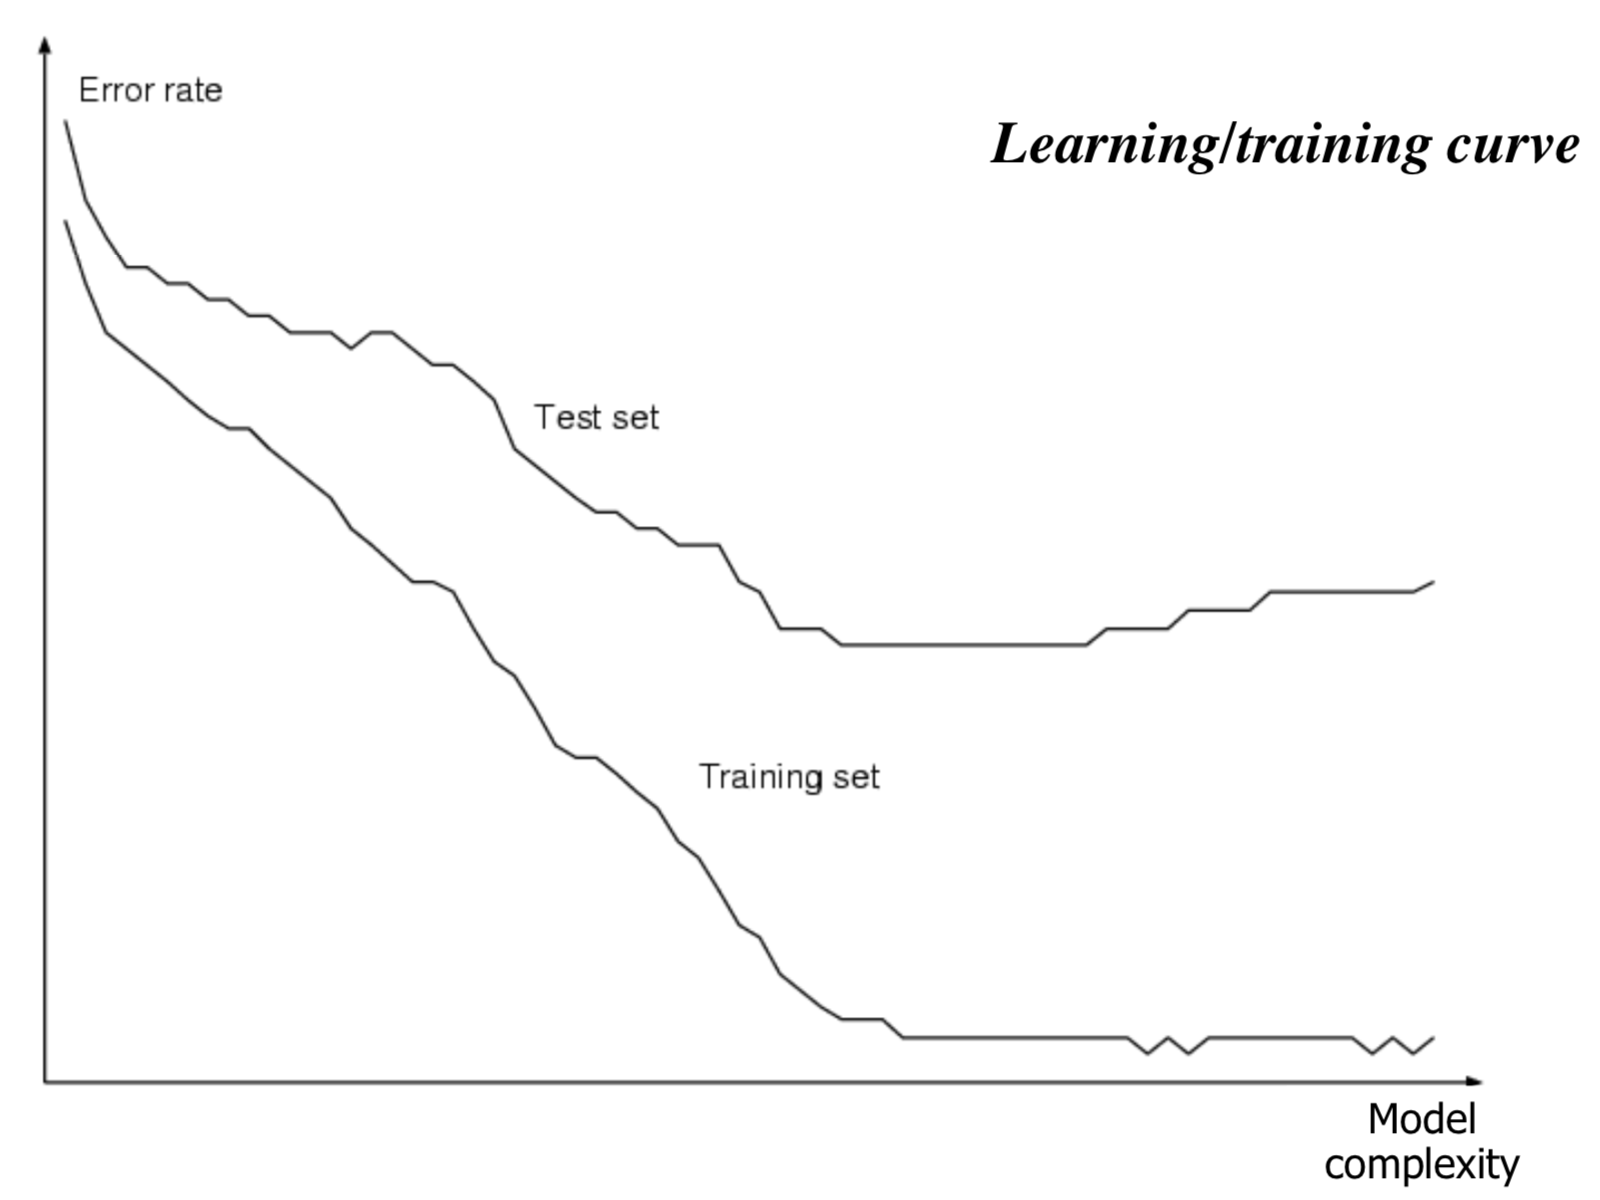
\includegraphics[scale=0.4]{Images/learntraincurve.png}
\end{figure}
All'inizio sia l'errore di training che quello di test sono alti, perché? Succede un po' quello che succedeva con il grado del polinomio troppo basso, che non fittava bene i dati $\rightarrow$ Underfitting. \newline
Alla fine invece l'errore di training é basso mentre l'errore sul test é alto, perché? É il caso in cui si sta overfittando sui dati di training e quindi il grado del polinomio é molto alto, ma non si sta comportando bene riguardo la generalizzazione sui dati di test sconosciuti.
\begin{figure}[H]
\centering
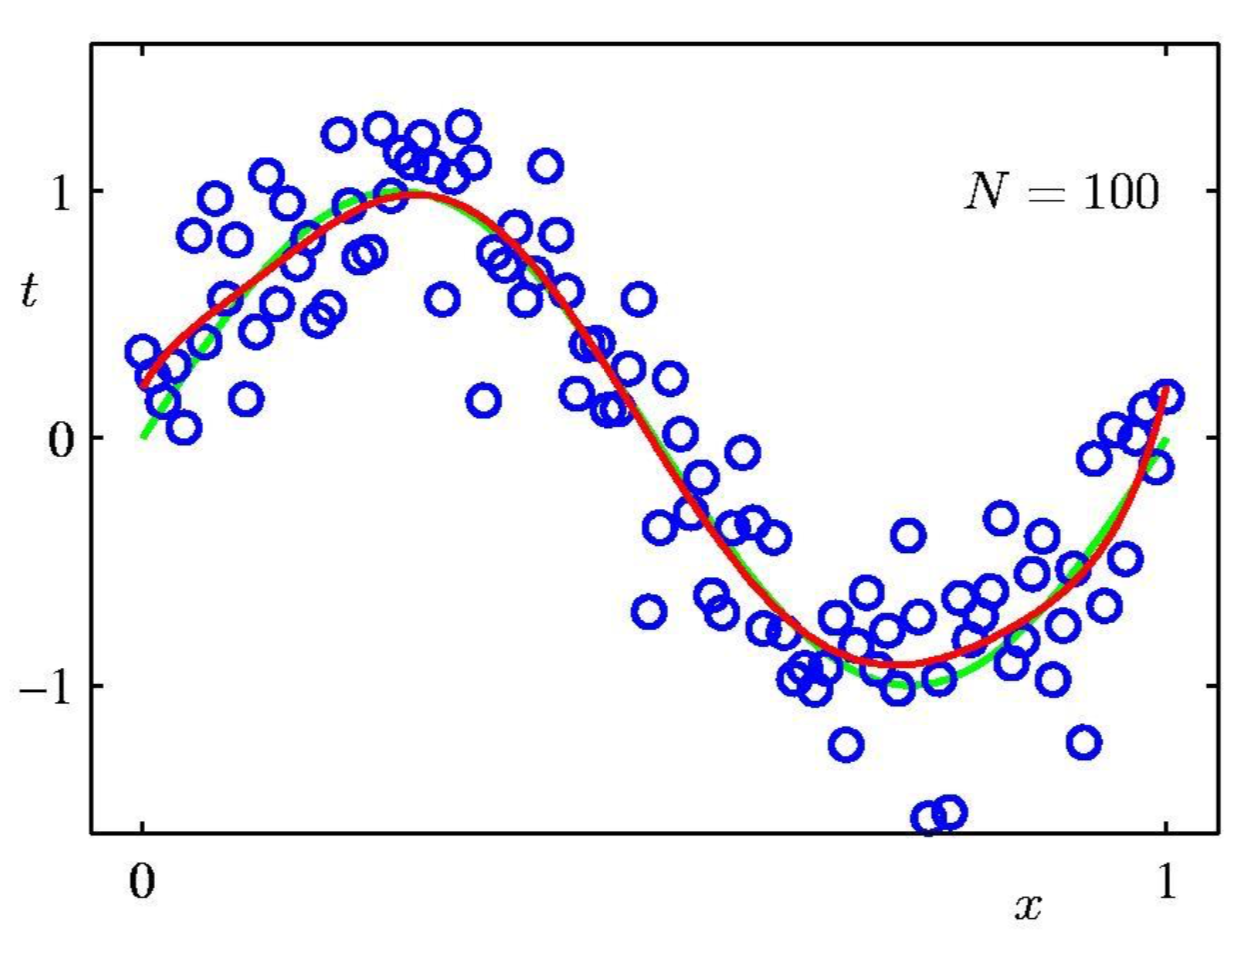
\includegraphics[scale=0.4]{Images/bigdatasethighpolgrade.png}
\end{figure}
Se prendiamo un polinomio con grado alto, ma abbiamo molti dati in più, predico meglio la funzione target. Ma quindi il problema era l'alto grado del polinomio o i pochi dati a disposizione? Per dare una risposta a questa domanda esiste della teoria di supporto.

\subsection{Statistical Learning Theory}
Mettendo insieme: 
\begin{itemize}
    \item La capacità di generalizzazione (misurata come errore di test) di un modello rispetto all'errore di addestramento delineando le zone di overfitting o underfitting
    \item Il ruolo della complessità del modello
    \item Il ruolo del numero di dati
\end{itemize}
troviamo la Statistical Learning Theory (SLT):
\begin{quote}
    \begin{itemize}
        \item si approssima una funzione sconosciuta f(x)
        \item si minimizza la funzione di rischio $R=\int L(t,h(x))dP(x,t)$ (Integrale della loss su tutti i dati).
        \item vengono dati un valore target $t$, una probabilitá di distribuzione $P(x,t)$ e una funzione Loss del tipo $L(h(x),t)=(t-h(x))^2$
        \item dobbiamo cercare h nello spazio delle ipotesi H, dove il valore di rischio generale R é minimo, ma noi abbiamo solo un data set finito $TR(x_i,t_i)$ con i=1...l
        \item per cercare h dobbiamo quindi minimizzare l'errore empirico (training error) trovando il miglior valore per il modello con parametri liberi w. \[R_{emp}=\frac{1}{l}\sum_{i = 1}^l (t_i-h(x_i))^2\]
    \end{itemize}
\end{quote}
Questo si chiama principio induttivo della minimizzazione del rischio empirico (Empirical Risk Minimization). La domanda che dobbiamo porci é: possiamo usare $R_{emp}$ per approssimare R?

\subsection{Teoria di Vapnik-Chervonenkis + SLT}
\begin{itemize}
    \item VC-dim é una misura per la complessità dello spazio delle ipotesi H (flessibilità per fittare i dati, come ad esempio il numero di parametri per modelli lineari/ grado del polinomio)
    \item VC-bounds afferma che con una probabilità di $1-\delta$ che \[ R \leq R_{emp} + \epsilon(\frac{1}{l},VC,\frac{1}{\delta})\]
    cioè che il rischio generale R ha un limite superiore definito dal rischio empirico (che decresce con la complessità dei modelli) più il VC-confidence. Il VC-confidence ($\epsilon$) aumenta all'aumentare della complessità del modello (indicata da VC) e diminuisce quando il numero dei dati aumenta. ($1/\delta$ indica la probabilitá che valga questo bound)
\end{itemize}
Possiamo usare il rischio empirico per approssimare R? Sì, il Machine Learning è ben fondato, l'intuizione sta nel fatto che un numero alto di dati portano ad un R basso, e un alto VC-dim abba $R_{emp}$ ma potrebbe alzare R (overfitting).
\subsection{Structural Risk Minimization}
\begin{figure}[H]
\centering
\includegraphics[scale=0.4]{Images/structuralriskmin.png}
\end{figure}
Sfruttiamo il concetto di controllo della complessità del modello, eseguiamo un trade-off tra la complessità del modello e l'accuratezza sul TR set.

\subsection{Conclusioni}
La STL permette di inquadrare formalmente il del problema della generalizzazione e overfitting, fornendo limitazioni superiori analitiche e quantitative al rischio R di predizione su tutti i dati, indipendentemente dal tipo di learning algorithm o dettagli del modello. Il ML e ben fondato, il rischio del learning (e l'errore di generalizzazione) può essere analiticamente limitato! Si puó trovare un buona approssimazione della f target da esempi, pur di avere un buon numero di dati e una adeguata complessità del modello (misurabile formalmente con la VC-dim). Questo ci porta a nuovi modelli (SVM) (e altri metodi che direttamente considerino il controllo della complessità nella costruzione del modello). Fonda uno dei principi induttivi sul controllo della complessità. \newline
Alcuni esempi di controllo della complessità sui modelli lineari sono il numero di parametri liberi w o la dimensione in input. Mentre per i decision trees il numero di nodi. Vedremo un approccio diretto alla complessità attraverso il modello SVM.

\section{Support Vector Machine}
Il Support Vector Machine (o SVM) é l'approccio più famoso per il supervised learning. É un classificatore derivato dalla statistical learning theory, dopo anni di sviluppi teorici, SVM é diventato famoso quando, usando immagini come input, dava una accuratezza comparabile a reti neurali.

\subsubsection{Obiettivi utilizzo SVM}
\begin{enumerate}
    \item Controllare la complessità del modello attraverso un approccio di ottimizzazione, approssimando la minimizzazione del rischio strutturale.
    \item Usare efficientemente l'espansione lineare via kernel in modo tale da ottenere un approccio flessibile per il supervised learning non lineare.
    \item Evitare di utilizzare SVM nel modo sbagliato.
\end{enumerate}

\subsection{Maximum Margin Classifier (controllo complessità)}
Viene utilizzato nella classificazione binaria di problemi, mettiamoci nel caso in cui abbiamo un sistema linearmente separabile, non tutti gli iper-parametri che risolvono la soluzione sono uguali
\begin{figure}[H]
\centering
\includegraphics[scale=0.4]{Images/svmmultiplesolution.png}
\end{figure}
Grazie a SVM abbiamo un criterio per scegliere le soluzioni: minimizzare il rischio strutturale.
\begin{figure}[H]
\centering
\includegraphics[scale=0.4]{Images/svmmargin.png}
\end{figure}
\begin{quote}
    Il margine é (il doppio della) la distanza tra l'iperpiano e il dato piú vicino.
\end{quote}
Notiamo che però non tutti gli iperpiani che risolvono il problema sono uguali, variando l'iperpiano anche il margine cambia.
\begin{figure}[H]
\centering
\includegraphics[scale=0.4]{Images/svmbigmargin.png}
\end{figure}
Ed é per questo motivo che cerchiamo il classificatore con il margine massimo!

\subsection{Rappresentazione canonica dell'iperpiano e Support Vector}
\begin{figure}[H]
\centering
\includegraphics[scale=0.4]{Images/svmmargincanonical.png}
\caption{nota: $w_0=b$}
\end{figure}
\begin{quote}
    Support Vectors: $x_i : |w^Tx_i+b|=1$
\end{quote}
Tutti i punti sonio classificati correttamente se $(w^Tx_i+b)y_i \geq 1 \quad \forall i$

\subsection{Verso l'ottimizzazione del margine}
Consideriamo il problema di apprendere un modello lineare per classificazione binaria \newline ($h(x)=sign(wx+b)$). Il problema consiste nel trovare i vettori (w,b) in modo tale che tutti i punti sono classificati correttamente e il margine é massimizzato. \newline
La rappresentazione canonica dell'iperpiano é definita come 
\begin{quote}
    il punto $(x_i,y_i)$ é classificato correttamente per tutti gli i (tutti gli esempi del training set) se:
    \begin{itemize}
        \item $w^Tx_i+b \geq 0$ se $y_i=1$
        \item $w^Tx_i+b \leq 0$ se $y_i=-1$
    \end{itemize}
    é possibile scalare w e b in modo tale che i punti più vicini all'iperpiano soddisfano $|w^Tx_i+b|=1$
\end{quote}
Due fatti a noi utili sono:
\begin{enumerate}
    \item Margine = $2/|w|$ e sappiamo anche che $|w|^2=(w^Tw)$. Quindi per minimizzare il margine $\rightarrow$ minimizzare $|w|$ $\rightarrow$ minimizzare $|w|^2/2$
    \item Il VC-dim del SVM é inversamente proporzionale al margine, quindi cotrolliamo la complessitá del modello utilizzando il margine
\end{enumerate}
Come abbiamo accennato precedentemente, l'iperpiano ottimo é l'iperpiano che massimizza il margine e ovviamente risolve il problema di training. 

\subsection{Problema di ottimizzazione quadratico}
Il nostro problema é quindi diventato 
\begin{quote}
    minimizzare $|w|^2/2$ in modo tale che $(wx_i+b)y_i\geq1$ per tutti gli i
\end{quote}
Nota: minimizzazione diretta della complessità del modello (funzione di ottimizzazione). Essendo il problema linearmente separabile abbiamo mantenere la soluzione (0 errori) nei vincoli. In relazione alla SLT minimizzando la VC-dim, diminuiamo anche il bound di errore.

\subsection{Nuovo classificatore h(x)}
\begin{quote}
    Dobbiamo massimizzare $\sum_i \alpha_i - \sum_{i,j} \alpha_i\alpha_j y_i y_j x_i^T x_j / 2$ con $\alpha_i \geq 0$. Cerchiamo un $\alpha_i$ ottimale.
\end{quote}
trovato il miglior alpha (calcolato dalla forma duale) possiamo calcolare $w=\sum \alpha_iy_ix_i$ e $b=y_k-w^Tx_k$ per qualsiasi $\alpha_k >0$. Possiamo adesso definirci un nuovo classificatore 
\begin{equation}
    h(x)=sign(w^Tx+b)=sign(\sum_{i=1}^l \alpha_iy_ix_i^Tx+b)=sign(\sum_{i \in SV} \alpha_iy_ix_i^T x+b)
\end{equation}
$x_i^Tx$ é il prodotto scalare tra le x dei vettori di supporto (presi ovviamente dal training set) e la x da classificare (quanto somiglia al valore di training, ci dice quanto matchano gli operandi)).
\begin{quote}
    $\alpha_i!=0$ allora $x_i$ é un support vector
\end{quote}
la soluzione é sparsa e formulata solo nei termini di SV. L'iperpiano dipende solo dai support vectors! Una forma speciale della soluzione in cui non dobbiamo nemmeno cacolare esplicitamente (w,b) per classificare i punti.
\begin{figure}[H]
\centering
\includegraphics[scale=0.4]{Images/hyperplanesv.png}
\end{figure}
\clearpage

\subsection{Margine Soft}
Purtroppo però, nella realtà, non abbiamo quasi mai dei problemi che sono linearmente separabili e con zero errore di classificazione. Anche se il problema fosse linearmente separabile, rischieremmo di avere un margine piccolissimo, quindi una VC-dimension molto alta, con tutti i problemi che ne conseguono. Ammettiamo quindi errore introducendo le slack-variables (variabili di rilassamento). 
\begin{quote}
    Le variabili slack $\xi_i$ possono essere aggiunte per permettere classificazioni errate o punti "molto rumorosi"
\end{quote}
\begin{figure}[H]
\centering
\includegraphics[scale=0.35]{Images/slackvar.png}
\end{figure}
Il nostro problema quindi é diventato 
\begin{quote}
    minimizzare $|w|^2/2+C\sum_i\xi_i$ tale che $(wx_i+b)y_i\geq 1-\xi_i$ e $\xi_i\geq0$ per ogni i
\end{quote}
Possiamo vedere $\xi$ come la distanza tra il vettore di supporto e il punto che stiamo analizzando, mentre $C>0$ gestisce il numero di errori permessi (C é un valore definito dall'utente). Con un C basso stiamo accettando tanti errori sul TR e quindi sfociare in un possibile underfitting. Con un C alto non permettiamo errori sul TR e quindi sfociare un un possibile overfitting. 

\subsection{Mapping per Spazi Dimensionali Ampi}
Cosa succede in casi non lineari? Dobbiamo utilizzare efficientemente l'espansione della base via kernel in modo tale da ottenere un approccio flessibile anche per il supervised learning non lineare. Mappare i dati in uno spazio dimensionale più grande permette di rendere linearmente separabili gli esempi.
\begin{figure}[H]
\centering
\includegraphics[scale=0.35]{Images/Mappingtohighdim.png}
\end{figure}
Ma questo lo sapevamo già, quando usavamo la funzione $\phi(x)$ al posto di x. 
\[ h_w(x)=sign(\sum_kw_k\phi_k(x))\]
Sappiamo che l'utilizzo di spazi ad alta dimensione (funzioni di espansione della base) può essere non conveniente nel calcolo dal punto di vista computazionale e può facilmente portare a un overfitting, nel caso in cui non controlliamo la dimensione dello spazio e la complessità del classificatore (la complessità in questo caso é correlata alla dimensionalità dell'input). Useremo l'approccio del Kernel per gestire (implicitamente) lo spazio nel contesto della modellizzazione regolarizzata (la complessità dipende dal margine). Pertanto, grazie alla regolarizzazione automatizzata di SVM, la complessità del classificatore può essere mantenuta ridotta indipendentemente dalla dimensionalità nel nuovo spazio. \newline
In SVM non é necessario calcolare w e nemmeno calcolare direttamente la $\phi$. Poiché sfruttiamo il Kernel. Il Kernel è il risultato del prodotto scalare. Non ci importa di come è fatta la phi: non ho bisogno di espanderla per poi fare il prodotto scalare, ma mi basta il risultato.
\[ h(x)=sign(\sum_{i\in SV} \alpha_iy_i\phi^T(x_i)\phi(x)) = sign(\sum_{i\in SV} \alpha_iy_iK(x_i,x))\]

\subsubsection{Esempi di Kernel}
\begin{itemize}
    \item Lineare: $K(x_i,x_j)=x_i^Tx_j$ \newline
        Mapping $\phi$: $x \rightarrow \psi(x)$ dove $\psi(x)$ é x stesso
    \item Polinomiale: $K(x_i,x_j)=(1+x_i^Tx_j)^p$ con p iper-parametro che indica il grado del polinomio \newline
        Mapping $\phi$: $x \rightarrow \psi(x)$ dove $\psi(x)$ ha dimensione esponenziale rispetto a p
    \item RBF (radial-basis-function) Gaussiana: $K(x_i,x_j)=e^{-||x_i-x_j||^2/2\sigma^2}$ dove $\sigma$ é un iper-parametro\newline
        Mapping $\phi$: $x \rightarrow \psi(x)$ dove $\psi(x)$ é di dimensione infinita \newline
        (molto potente sul TR ma puó portare ad overfitting)
\end{itemize}

\subsection{Riassunto procedimento SVM}
\begin{itemize}
    \item Scegliamo un parametro C (trade-off)
    \item Scegliamo una funzione di Kernel K (e i suoi parametri)
    \item Troviamo il mglior $\alpha$
    \item Usiamo il modello finale \[h(x)=sign(\sum_{i\in SV} \alpha_iy_iK(x_i,x))\]
\end{itemize}

\subsection{Utilizzare bene SVM}
Evitare errori di interpretazione tipici nell'uso di SVM. È possibile che si verifichi un overfitting senza un'attenta selezione dei parametri: C, funzione Kernel, parametri del Kernel, ecc... Il trattamento implicito dello spazio grande deve avvenire nello spazio delle caratteristiche e non in quello di input. Anche la tecnica di validation vista fino ad ora per la selezione del modello e la valutazione del modello devono essere utilizzate rigorosamente.\clearpage
Quindi:
\begin{itemize}
    \item Trasformare i dati in un formato leggibile da un software SVM (ad esempio \{red, green, blue\} $\rightarrow$ (0,0,1), (0,1,0), (1,0,0))
    \item Eseguire una semplice scalatura dei dati (ad esempio in un intervallo da [-1,1] o [0,1]
    \item Considerare il kernel $K(x_i,x_j)=e^{-||x_i-x_j||^2/2\sigma^2}$
    \item Usare la cross-validation per trovare i migliori parametri C e $\sigma$
    \item Riutilizzare il TR set peró con i migliori C e $\sigma$ trovati
    \item Eseguire il testing su un Test Set esterno
\end{itemize}

\section{K-Nearest Neighbors}
K-NN fa parte del supervised learning, vediamo la forma piú semplice di questo metodo basato su istanze.

\subsection{1-Nearest Neighbor}
Questo algoritmo non impara, ma sfrutta tutti i valori del training set.
\begin{itemize}
    \item Salvare i dati di training nella forma $<x_j,y_j>$ con j=1...l
    \item Dato un input x di dimensione n:
    \begin{itemize}
        \item Trovare l'esempio di training più vicino $x_i$ tale che $d(x,x_i)$ é minimo \newline
        dove \[d(x,x_j)=\sqrt{\sum_{t=q}^n(x_t-x_{jt})^2}=||x-x_j||\] $x_t$ é la componente t-esima di x, $x_{jt}$ é la componente t-esima di $x_j$
    \end{itemize}
    \item Diamo come output $y_i$ (in pratica stiamo vedendo l'esempio che piú assomiglia ai nostri dati e rispondiamo come ha risposto lui
\end{itemize}
\begin{figure}[H]
\centering
\includegraphics[scale=0.4]{Images/1-nn.png}
\end{figure}
É molto flessibile, non c'è errore di classificazione sui dati di TR, il decision boundary non é piú lineare e potrebbe portare all'overfitting?

\subsection{K-NN}
\begin{figure}[H]
\centering
\includegraphics[scale=0.4]{Images/5-nn.png}
\end{figure}
Vediamo già come si comporta in questo caso 1-nn risponderebbe + per $x_q$, valutando invece con 5-nn viene restituito - per $x_q$. Come succedeva con il polinomio di alto grado che andava in overfitting, anche qui dobbiamo renderlo più "smooth" valutando su un insieme di vicini. \newline
Per questo possiamo "dare un occhiata" a tot (k) vicini e restituire una media: \[avg_k(x)=\frac{1}{k}\sum_{x_i\in N_k(x)} y_i\] dove $N_k(x)$ é il vicinato di x che contiene esattamente k vicini. Se c'è una chiara dominanza di una delle classi nel vicinato di x, allora é probabile che anche x appartenga a quella classe. Quindi la regola di classificazione è la maggioranza che vota tra i membri di $N_k (x)$. \[h(x)=1 \text{ se } avg_k(x)>0.5 \text{      0 altrimenti}\]

\begin{figure}[H]
\centering
\includegraphics[scale=0.4]{Images/15-nn.png}
\end{figure}

Dobbiamo trovare il giusto trade-off tra underfitting e overfitting trovando il giusto valore k. (Nota: é possibile usare k-nn anche se ci sono piú classi). \newline
\subsection{Considerazioni su K-nn}
Non c'è una ipotesi globale per tutte le istanze: non c'é quindi nessun modello da allenare. Dobbiamo semplicemente memorizzare gli esempi di input, inoltre il modello non é parametrico. Si tratta di una stima lineare globale della funzione target (sullo spazio dell'istanza). É un metodo basato sulla memoria, sull'istanza e sulla distanza, Bias induttivo! scegli il risultato in base alla distanza. \newline
Notare che k-nn fa una approssimazione locale della funzione target per ogni nuovo esempio da classificare, il costo computazionale é tutto contenuto nella fase di predizione. Inoltre é molto costosto a livello computazionale perché per ogni nuovo input bisogna calcolare le distanze dall'esempio a tutti i vettori memorizzati. Il tempo è proporzionale al numero di modelli memorizzati, questo ci fa notare che anche il costo per lo spazio é alto, dato che tutti i dati sono memorizzati. \newline
Quando abbiamo molte variabili in input k-nn spesso fallisce a causa del "curse of dimensionality": quando la dimensione aumenta, il volume dello spazio aumenta in modo tale che i dati disponibili diventano sparsi. Ad esempio la quantitá di dati che servono per supportare un risultato spesso cresce esponenzialmente con la dimensione. Troviamo anche il problema denominato "curse of noisy": se il target dipende da poche altre variabili, potremmo trovarci un "modello simile" con la somiglianza dominata dal gran numero di funzioni irrilevanti. 

\subsection{Distance Based methods}
Quando utilizzo degli approcci basati su distanza (come k-nn o alcune funzioni kernel) devo assicurarmi che la distanza calcolata sia davvero un fattore discriminante. Stiamo misurano quando una coppia di pattern si assomiglia, inoltre dare una metrica pone un bias rilevante sulla soluzione e la metrica dipende da un dominio (es due stringhe in un linguaggio). Possiamo imparare in qualche modo la metrica? Si (NN, Learning K...). 

\section{Unsupervised Learning (ripasso)}
Nel Unsupervised Learning non abbiamo esempi etichettati, e quindi con un output associato, siamo noi come sistema di apprendimento che dobbiamo trovare correlazioni tra i dati e raggrupparli (clustering). Dobbiamo quindi ripartire i dati, in cluster (sottoinsiemi di dati simili). Il goal che ci poniamo é ripartire in modo ottimo una distribuzione sconosciuta di dati, in uno spazio di dimensione x, in regioni (approssimando poi usando un cluster). In questo caso H é un insieme di quantizzatori di vettori $x\rightarrow c(x)$ cioè dato un vettore in input voglio sapere a quale cluster appartiene. Passiamo da uno spazio continuo ad uno spazio spazio discreto. \newline 
Una funzione di Loss comune é \[L(h(x_i))=||x_i-c(x_i)||^2\] cioè la distanza tra x e il centroide. Il valore medio sulla distribuzione degli input è l'errore di quantizzazione. \newline
Unsupervised Learning viene spesso usato in Data Analysis per scoprire caratteristiche comuni tra i dati, viene anche usato per il Preprocessing dei dati da utilizzare poi in seguito per altri approcci di ML. Inoltre dobbiamo notare il fatto che raccogliere dati non etichettati é più "economico", rispetto a trovarne labeled.

\subsection{K-means}
K-means fa parte del Unsupervised Learning. Il K-means è l'algoritmo più semplice e più comunemente usato che utilizza un criterio di errore al quadrato. L'algoritmo K-means è popolare perché è facile da implementare ed è generalmente efficiente, tuttavia, presenta diversi inconvenienti e limitazioni che vedremo dopo...
\begin{enumerate}
    \item Scegliere k centri di cluster in modo che coincidano con k modelli scelti casualmente (o k punti definiti casualmente all'interno dell'ipervolume contenente il set di pattern) \newline
    $c_1...c_k$ con k fissato che scegliamo noi.
    \item Assegnare ad ogni modello il centro del cluster più vicino (il vincitore) \newline
    per ogni x calcoliamo
    \[i^*(x)=argmin_i||x-c_i||^2=\sum_{j\rightarrow n}(x_j-c_{ij})^2\]
    cioè provo tutti i $c_i$ e quello che ha distanza minima é il vincitore (mi interessa l'indice del vincitore $i^*$). Adesso x appartiene al cluster $i^*$
    \item Ricalcolare i centri del cluster (centroide) utilizzando le nuove appartenenze al cluster corrente
    \[c_i=\frac{1}{|\text{num di membri cluster}_{i}|}\sum_{x_j \in cluster_i}x_j\]
    \item Se non viene soddisfatto un criterio di convergenza, andare al passaggio 2 (criteri come nessuna (o minima) riassegnazione di schemi a nuovi centri di cluster o una minima diminuzione dell'errore quadratico)
\end{enumerate}
\begin{figure}[H]
\centering
\includegraphics[scale=0.25]{Images/k-means-1.png}
\includegraphics[scale=0.25]{Images/k-means-2.png}
\includegraphics[scale=0.25]{Images/k-means-3.png}
\includegraphics[scale=0.25]{Images/k-means-4.png}
\includegraphics[scale=0.25]{Images/k-means-5.png}
\end{figure}

\subsection{Limitazioni K-means}
Il numero di cluster da trovare deve essere fornito (questo porta a fare trial and error per trovare il K che fitta meglio). I minimi locali della Loss rendono il metodo dipendente dall'inizializzazione, si esegue più volte da diverse inizializzazioni casuali (ci sono anche dei metodi che inizializzano con un'euristica). K-means può funzionare bene per cluster compatti, ma non consente di proiettare i dati in uno spazio di dimensione minore. \newline
Come viene valutato l'output di un algoritmo di clustering? Che cosa caratterizza un risultato di raggruppamento "buono" e uno "scarso"? Nel clustering esiste ben poco in termini di "standard di riferimento", tranne nei sottodomini specifici in cui conosco la metrica (conosco bene il problema e so riconoscere una classificazione sensata). Misure oggettive (non trattate qui) come ad esempio l'errore di quantizzazione. Noi sappiamo a quali classi appartengono i dati, ma usiamo un algoritmo di clustering, e controlliamo che le classi corrispondano. È un modo sbagliato per valutare la bontà di un algoritmo di clustering!

\subsection{Preprocessing dei dati}
Abbiamo visto che Unsupervised Learning viene utilizzato per il preprocessing dei dati, ma in che modo?
Menzioniamo la riduzione della dimensionalità cioè trasformare la dimensione dei dati in una più piccola. (non é importante la quantità, bensì la dimensione dei dati!) \newline
$<x_1, x_2, ..., x_n> \rightarrow <x'_1, x'_2, ..., x'_m>$ con $n>m$. \newline
Un esempio é il PCA (principal component analysis) dove i nuovi assi sono calcolati nella direzione di massima varianza dei dati 
\begin{figure}[H]
\centering
\includegraphics[scale=0.4]{Images/PCA.png}
\end{figure}
Un altro approccio per il preprocessing dei dati é la feature selection: é una particolare tecnica di riduzione della dimensionalità nella quale scelgo le variabili più significative per il task, anziché trasformarle. In pratica scegliamo un sottoinsieme di tutte le caratteristiche. Un ultimo approccio dal preprocessing che vediamo é Outlier detection: si cercano valori inusuali dei dati che non sono consistenti con gli altri (valori scorretti a causa di misurazioni errate).

\section{Altri Task del Machine Learning}
Altri task che non fanno parte del supervised o unsupervised learning.
\begin{itemize}
    \item Reinforcement Learning: si utilizza come metodo di adattamento per sistemi autonomi (in particolare in robotica). L'algoritmo apprende un criterio su come agire data un'osservazione del mondo. Ogni azione ha un certo impatto sull'ambiente e l'ambiente fornisce un feedback che guida l'algoritmo di apprendimento. Invece di avere una supervisione per ogni passaggio, abbiamo informazioni su vittorie / perdite per lo stato finale. Le azioni devono massimizzare la quantità di vittorie ricevute. L'apprendimento decide quali azioni sono state maggiormente responsabili di vittorie / perdite.
    \item Semi-Supervised Learning: combina esempi etichettati e non etichettati (in genere in numero maggiore) per generare una funzione o un classificatore appropriati.
    \item Learn to Rank: (utilizzato per i motori di ricerca) quando l'input è un insieme di oggetti e l'output desiderato è una classifica (un ranking) di tali oggetti.
    \item On-Line Learning: nuovi esempi sono imparati al momento
    \item Structured domain learning and relational learning: il dominio di input e output può essere strutturato sotto forma di sequenze (segnali, serie temporali, ...) o in modo più complesso: alberi, grafici, reti sociali.
\end{itemize}

\section{Altri Modelli del Machine Learning}
\subsection{Reti Neurali}
Vengono utilizzate sia nel Supervised che nel Unsupervised Learning. Sono simili alla visione del Linear Threshold Unit, una rete neurale é una rete di modelli non lineari con una capacità di approssimazione universale e capacità predittive. Gli strati interni sono "nascosti", e ogni unità é non lineare, fornendo alla rete neurale la capacità di estrarre (imparando) una nuova rappresentazione dei dati. Questa nuova rappresentazione semplifica il compito di classificazione nell'ultimo livello della rete. \newline 
Abbiamo una espansione della base non lineare in w, e le $\phi$ sono imparate automaticamente, ma purtroppo questo scaturisce in un problema di ottimizzazione non lineare. 
\begin{figure}[H]
\centering
\includegraphics[scale=0.4]{Images/NN.png}
\end{figure}
\subsection{Deep Learning}
Il Deep Learning è quel campo di ricerca dell'apprendimento automatico (machine learning) e dell'intelligenza artificiale che si basa su diversi livelli di rappresentazione, corrispondenti a gerarchie di caratteristiche di fattori o concetti, dove i concetti di alto livello sono definiti sulla base di quelli di basso. In altre parole, si intende un insieme di tecniche basate su reti neurali artificiali organizzate in diversi strati, dove ogni strato calcola i valori per quello successivo affinché l'informazione venga elaborata in maniera sempre più completa. \newline
Piú tecnincamente, quando si parla di Deep Learning, si fa riferimento a reti neurali multistrato profonde, nel senso che abbiamo molteplici layer di unità di processing non lineari. Indipendentemente se si usa il Supervised o Unsupersised Learning per la rappresentazione di caratteristiche in ogni livello, i vari livelli vanno a formare una gerarchia di caratteristiche / rappresentazioni da basso livello ad alto livello (diversi livelli di astrazione).
Imparare automaticamente come rappresentare i dati, e capire come classificarli aumenta il livello di astrazione tra i vari layer. Ad esempio, un'immagine può essere rappresentata in molti modi: come un vettore di pixel o in un modo più astratto come un insieme di bordi, regioni di forma particolare, ecc... Per questo il Deep Learning funziona meglio quando i dati in input hanno una sorta di struttura: spaziale, temporale, linguistica ecc...
\begin{figure}[H]
\centering
\includegraphics[scale=0.4]{Images/deeplearningimage.png}
\end{figure}
I vantaggi del Deep Learning sono svariati, come ad esempio la possibilità di sfruttare la composizionalitá della rappresentazione interna: guadagno esponenziale nel potere di rappresentazione. I concetti più semplici vengono rappresentati in uno strato della rete, i quali poi possono essere sfruttati come dati primitivi dal livello successivo, per rappresentare concetti più complessi. Sono necessari meno esempi per raggiungere una buona capacità di generalizzazione! Le Deep Networks erano difficili da addestrare in passato, ma combinando tecniche per l'addestramento di modelli grandi, HPC (ad esempio GPU) e grandi raccolte di dati da applicazioni reali (ad esempio milioni di immagini), al giorno d'oggi lavorano molto bene conseguendo una rivoluzione nell'approccio AI alle soluzioni del mondo reale.







%\bibliographystyle{plain}
%\bibliography{references}
\end{document}
